\documentclass[11pt,letterpaper]{article}

\makeatletter
\renewcommand\paragraph{\@startsection{paragraph}{4}{\z@}%
                                      {1ex \@plus1ex \@minus.2ex}%
                                      {-1em}%
                                      {\normalfont\normalsize\bfseries}}
\makeatother

%%%%%%%%%%%%%%%%%%%%%
%  P A C K A G E S  %
%%%%%%%%%%%%%%%%%%%%%

% Authors
\usepackage{authblk}

% Page margins
\usepackage[margin=1in]{geometry}

% Nicer math font
\usepackage{mathpazo}

% More fancy lists
\usepackage{enumerate}

% Microtype
\usepackage{microtype}

% TikZ
\usepackage{tikz}
%\usetikzlibrary{calc,shapes.geometric}
\usetikzlibrary{backgrounds,fit,decorations.pathreplacing,calc}

% Highlights
\usepackage{soul}


% Figure
\usepackage{float}

% Hypertext package
\usepackage[colorlinks = true]{hyperref}
% Title and authors
%\hypersetup{
%  pdftitle = {},
%  pdfauthor = {}
%}
% Color definitions
\definecolor{darkred}  {rgb}{0.5,0,0}
\definecolor{darkblue} {rgb}{0,0,0.5}
\definecolor{darkgreen}{rgb}{0,0.5,0}
% Color links
\hypersetup{
  urlcolor   = blue,         % color of external links
  linkcolor  = darkblue,     % color of internal links
  citecolor  = darkgreen,    % color of links to bibliography
  filecolor  = darkred       % color of file links
}

% AMS
\usepackage{amsmath,amssymb,amsfonts,amsthm,amstext}

%% Restating theorems
%\usepackage{thm-restate}

% Powerful macros
\usepackage{etoolbox}

% Fixes for amsmath
\usepackage{mathtools}
\mathtoolsset{centercolon}
\makeatletter
\protected\def\tikz@nonactivecolon{\ifmmode\mathrel{\mathop\ordinarycolon}\else:\fi}
\makeatother

% Daw boxes
\usepackage{tcolorbox}

% Code
\usepackage{algorithm}
%\usepackage{algorithmic}
\usepackage{algpseudocode}

% Clever references

\usepackage{cleveref}%[nameinlink]


\crefname{lemma}{Lemma}{Lemmas}
\crefname{proposition}{Proposition}{Propositions}
\crefname{definition}{Definition}{Definitions}
\crefname{theorem}{Theorem}{Theorems}
\crefname{conjecture}{Conjecture}{Conjectures}
\crefname{corollary}{Corollary}{Corollaries}
\crefname{claim}{Claim}{Claims}
\crefname{section}{Section}{Sections}
\crefname{appendix}{Appendix}{Appendices}
\crefname{figure}{Fig.}{Figs.}
\crefname{table}{Table}{Tables}


% \crefname{algorithm}{Algorithm}{Algorithms}

% IEEE tools
\usepackage[retainorgcmds]{IEEEtrantools}

% table of contents
\usepackage{tocloft}

% Table with multi-row
\usepackage{multirow}

% TikZ
\usepackage{tikz}	
\usetikzlibrary{backgrounds,fit,decorations.pathreplacing}

%%%%%%%%%%%%%%%%%%%%%%%%%
%  N E W C O M M A N D  %
%%%%%%%%%%%%%%%%%%%%%%%%%

% Standard quantum notation

\newcommand{\ket}[1]{|#1\rangle}
\newcommand{\bra}[1]{\langle#1|}
\newcommand{\braket}[2]{\langle#1|#2\rangle}
\newcommand{\ketbra}[2]{|#1\rangle\langle#2|}
\newcommand{\proj}[1]{|#1\rangle\langle#1|}

\newcommand{\x}{\otimes}
\newcommand{\xp}[1]{^{\otimes #1}}
\newcommand{\op}{\oplus}

\newcommand{\ct}{^{\dagger}}
\newcommand{\tp}{^\intercal}

% Linear algebra

%\newcommand{\1}{\mathbb{1}} % identity matrix
%\DeclareMathOperator{\Hom}{Hom}
\DeclareMathOperator{\End}{End}
%\DeclareMathOperator{\E}{\mathbb{E}}
\DeclareMathOperator{\Lin}{L} % all linear maps
\newcommand{\Mat}[1]{\mathrm{M}(#1)} % all matrices
%\newcommand{\Mat}[1]{\mathrm{M}_{#1}(\C)}

% Paired delimiters

\DeclarePairedDelimiter{\set}{\lbrace}{\rbrace}
\DeclarePairedDelimiter{\abs}{\lvert}{\rvert}
\DeclarePairedDelimiter{\norm}{\lVert}{\rVert}
\DeclarePairedDelimiter{\cnorm}{\lvert}{\rvert}
\DeclarePairedDelimiter{\of}{\lparen}{\rparen}
\DeclarePairedDelimiter{\sof}{\lbrack}{\rbrack}
\DeclarePairedDelimiter{\ip}{\langle}{\rangle}
\DeclarePairedDelimiter{\floor}{\lfloor}{\rfloor}

% Operators

\renewcommand{\Re}{\operatorname{Re}}
\renewcommand{\Im}{\operatorname{Im}}
\DeclareMathOperator{\vc}{vec}
\DeclareMathOperator{\spn}{span}
\DeclareMathOperator{\rank}{rank}
\DeclareMathOperator{\diag}{diag}
\DeclareMathOperator{\spec}{spec}
\DeclareMathOperator{\Tr}{Tr}
\DeclareMathOperator{\sgn}{sgn}
\DeclareMathOperator{\hook}{hook}
\DeclareMathOperator{\E}{\mathbb{E}}
\DeclareMathOperator{\supp}{supp}


% Sets

\newcommand{\C}{\mathbb{C}}
\newcommand{\R}{\mathbb{R}}
\newcommand{\N}{\mathbb{N}}
\newcommand{\Z}{\mathbb{Z}}
\newcommand{\calH}{\mathcal{H}}
\newcommand{\calX}{\mathcal{X}}
\newcommand{\calY}{\mathcal{Y}}
\newcommand{\calA}{\mathcal{A}}
\newcommand{\calB}{\mathcal{B}}

% Group
\newcommand{\Zd}{\Z_d^{\times}}


% Identity operator
\newcommand{\1}{\mathbb{1}}

% Pauli Group
\newcommand{\Pg}{\mathcal{P}}
\newcommand{\J}{\mathcal{J}}

% Special notation

\newcommand{\CHSH}{CHSH^{(d)}}
\newcommand{\MS}{MS}
\newcommand{\EXT}{EXT}
\newcommand{\LS}{LS}
\newcommand{\COMM}{COMM}
\newcommand{\EPR}[1]{\Sigma^{(#1)}}
\newcommand{\paulix}{\sigma_x}
\newcommand{\pauliz}{\sigma_z}
\newcommand{\tP}{\tilde{P}}
\newcommand{\tQ}{\tilde{Q}}
\newcommand{\tM}{\tilde{M}}
\newcommand{\tN}{\tilde{N}}
\newcommand{\tA}{\tilde{A}}
\newcommand{\tB}{\tilde{B}}
\newcommand{\tX}{\tilde{X}}
\newcommand{\tZ}{\tilde{Z}}
\newcommand{\tU}{\tilde{U}}
\newcommand{\tW}{\tilde{W}}
\newcommand{\tx}{\tilde{x}}
\newcommand{\tpsi}{\tilde{\psi}}
\newcommand{\tri}{\Delta}
\newcommand{\lB}{\overline{B}}
\newcommand{\dr}[1]{d^{(#1)}}
\newcommand{\nr}{n(r)}
\newcommand{\mr}{m(r)}
\newcommand{\ux}{\underline{x}}
\newcommand{\uc}{\underline{c}}
\newcommand{\ua}{\underline{a}}
\newcommand{\ub}{\underline{b}}
\newcommand{\fC}{\mathfrak{C}}
\newcommand{\ba}{\pmb{a}}
\newcommand{\bb}{\pmb{b}}
\newcommand{\bc}{\pmb{c}}
\newcommand{\bS}{\mathrm{S}}

% Probabilities
\newcommand{\pr}[2]{P(#1|#2)}
\newcommand{\pa}[2]{P_A(#1|#2)}
\newcommand{\pb}[2]{P_B(#1|#2)}
\newcommand{\tpr}[2]{\tilde{P}(#1|#2)}

% Bell Ineqaulities
\newcommand{\I}{\mathcal{I}}

% Square root of epsilon
\newcommand{\ep}{\epsilon}
\newcommand{\se}{\sqrt{\epsilon}}
\newcommand{\qe}{\epsilon^{1/4}}
\newcommand{\sd}{\sqrt{d}}
\newcommand{\sr}{\sqrt{r}}
\newcommand{\qr}{r^{1/4}}
\newcommand{\qd}{d^{1/4}}

% Approximately equatli
\newcommand{\appd}[1]{\simeq_{#1}}

% Comments
\def\carl#1{{\color{blue} #1}}
\newcommand{\hf}[1]{\textcolor{red}{#1}}
\newcommand{\hfc}[1]{\textcolor{red}{#1 -H.F.}}

%%%%%%%%%%%%%%%%%%%%%%%%%
%  N E W T H E O R E M  %
%%%%%%%%%%%%%%%%%%%%%%%%%

\newtheorem{theorem}{Theorem}[section]
\newtheorem{lemma}[theorem]{Lemma}
\newtheorem{proposition}[theorem]{Proposition}
\newtheorem{definition}[theorem]{Definition}
\newtheorem{corollary}[theorem]{Corollary}
\newtheorem{conjecture}[theorem]{Conjecture}
\newtheorem{claim}[theorem]{Claim}
\newtheorem*{conjecture*}{Conjecture}
\newtheorem*{problem}{Problem}
\newtheorem*{example}{Example}

\theoremstyle{definition}
\newtheorem*{remark}{Remark}



%%%%%%%%%%%%%%%%
%   Document   %
%%%%%%%%%%%%%%%%

\begin{document}

\title{Constant-sized correlations are sufficient to 
robustly self-test maximally entangled states with unbounded dimension}

\author[1]{Honghao Fu}
\author[1,2]{Carl Miller}

\renewcommand\Affilfont{\itshape\small}



\affil[1]{Department of Computer Science, Institute for Advanced Computer Studies, and Joint Center for Quantum \break Information and Computer Science, University of Maryland, College Park, MD 20742, USA}
\affil[2]{National Institute of Standards and Technology, 100 Bureau Dr., Gaithersbug, MD 20899, USA}
\maketitle

\begin{abstract}
	We show that for any prime odd integer $d$ with primitive $r$, there exists a correlation of size
	$\Theta(r^2)$ 
	that can robustly self-test a maximally entangled state of dimension $4d-4$. Our result is
	inspired by the robust self-testing result by Bamps and Pironio (\textit{Physical Review A} $91.5$ $(2015)$) and
	techniques introduced by Slofstra (\textit{Forum of Mathematics, Pi}. Vol. $7$, $2019$). Since there are
	infinitely many prime numbers with primitive root at most $5$ (\textit{The Mathematical Intelligencer} $10.4$ ($1988$)), 
	our result implies that constant-sized correlations are sufficient for robust self-testing of maximally entangled states
	with unbounded local dimension.
\end{abstract}
%========================================
\section{Introduction}
\label{sec:intro}
%========================================
Self-testing is a unique phenomenon of quantum mechanics.
It is also powerful because only classical interactions are required.
It has many applications in quantum
delegated computation \cite{ruv2013,coladan2017verifier} and device independent quantum cryptography
\cite{mayersyao,vv2014,miller2017,fu2018,eat2018}.

The case of self-testing $2$-dimensional EPR pair, which is defined by
\begin{align*}
    \ket{EPR} = \frac{1}{\sqrt{2}}(\ket{00}+\ket{11}),
\end{align*}
is fully understood.
The techniques for robustly self-testing $\ket{EPR}$ is 
first introduced in Ref.~\cite{mckague2012}, then improved in Ref.~\cite{bamps2015}. 
Ref.~\cite{yang2013} proved an generalized swap-isometry
that can be used to robustly self-test large dimensional maxially entangled states.
Its ideas are realized later in Ref.~\cite{coladan2017all}, 
which proved that all pure bipartite entangled state 
can be self-tested.
The authors constructed a family of correlations such
that each partially or maximally entangled state of any local dimension has
a self-testing correlation in this family.
% One can also self-test many copies of the $2$-dimensional EPR
% pair in parallel \cite{mckague2016,natarajan2017,coladan2016parallel}.
% The most efficient way uses $O(\log n)$ bits question and
% answers to self-test $n$ copies of $2$-dimensional EPR
% pair \cite{lowdegree}.
% Self-testing general $d$-dimensional EPR pairs is a harder task.
% Coladangelo, Goh and Scarani has shown that all pure bipartite entangled states can be self-tested \cite{coladan2017all}
To generate a correlation in the family, Alice and Bob
have constant number of measurement settings but each 
measurement setting has the same number of outcomes as
the local dimension of the entangled state to be self-tested. 
In other words, their correlation is of size $\Theta(d^2)$,
where $d$ is the local dimension of the entangled state.
This is the only result about self-testing the general $d$-dimensional entangled state so far.
However, proving the robustness of the family of correlations remains an open problem. 
Without robustness, we cannot infer anything about a quantum strategy if
the produced correlation deviates from the ideal correlation, no matter how small the 
deviation is. 
 
A natural question to ask is whether maximally entangled states with large local dimension
can be robustly self-tested with constant-sized correlations. 
In this paper, we give an affirmative answer to this question by proving the following theorem.
\begin{theorem}[Informal]
\label{thm:inf}
	There exists an infinite-sized set $D$ of odd prime numbers such that, for any $d \in D$, 
	the maximally entangled state of local dimension $4(d-1)$ can be robustly self-tested 
	with constant-sized question and answer alphabets.
\end{theorem}
The formal statement of this theorem is given in \cref{thm:self-test} and \cref{thm:infty}.

The set $D$ is, specifically, the set of all 
odd prime numbers whose smallest primitive root is either $2$, $3$, or $5$.  
It has been shown that this set has infinitely many elements \cite{murty1988}.
To prove \cref{thm:inf}, we construct a correlation of size $\Theta(r)$ 
for each $d \in D$ whose smallest primitive root is $r$.
This correlation is denoted by $\fC(d,r)$.
Note that although the size of $\fC(d,r)$ does not depend on $d$, the entries of $\fC(d,r)$ do.
Then we prove the robust self-testing property of $\fC(d,r)$ by showing 
that if some quantum strategy can approximate $\fC(d,r)$, then
the generalized swap isometry \cite{yang2013}
can produce the desired maximally entangled states when applied to the unknown state used in the strategy.
%Then the self-testing property of this correlation is 
%given in the following theorem.
%\begin{theorem}[Informal]
%\label{thm:pr_2}
%	All maximally entangled state with local dimension $d-1$, where $d$ is prime and has
%	primitive root $r \in \{2, 3, 5\}$, can be self-tested by a constant-sized correlation.
%\end{theorem}
\carl{The paper \cite{bamps2015} says that the earlier paper \cite{yang2013} has ``flaws.'' Check what those flaws are, and make sure that they won't put a shadow on anything that you're discussing when you cite \cite{yang2013}.} 
\hfc{The flaws are in the self-testing proof, not in the 
proof about the generalized isometry.}

The correlation $\fC(d,r)$ contains the ideal correlation of a specially-designed binary linear system game.
In a general linear system game, Alice is given a random equation 
from a linear system and she
should give an assignment of the equation.
Bob is asked to assign a value to a random variable of that equation.
They win the game if Alice's assignment satisfies the equation and Bob's
assignment to the variable matches Alice's assignment.
A widely-used and thoroughly-studied example of a linear system game is
the Magic Square game \cite{magic_square}.
In this game, the linear system is
\begin{align*}
    &x_1 + x_2 + x_3 = 0 && x_4 + x_5 + x_6 = 0 &&
    x_7 + x_8 + x_9 = 0 \\
    &x_1 + x_4 + x_7 = 0 && x_2 + x_5 + x_8 = 1 &&
    x_3 + x_6 + x_9 = 0.
\end{align*}
Using two copies of the maximally entangled state
\begin{align*}
    \ket{EPR} = \frac{1}{\sqrt{2}}(\ket{00}+\ket{11}),
\end{align*}
the Magic square game can be won
with certainty.
It has been shown that if a strategy that can win this game almost perfectly, the shared state must be close to $\ket{EPR}^{\x 2}$ up to some local isometry \cite{wu2016}, 
so we can say that the Magic Square game can robustly self-test $\ket{EPR}^{\x 2}$.
The key observation that leads to the self-testing proof is that 
a winning strategy must contain observables $X$ and $Z$ that 
satisfy the anti-commutation relation 
\begin{align*}
    X Z = - Z X.
\end{align*}
Intuitively, we can think of the Magic Square game as a way to enforce the
anti-commutation relation.

Our linear system game is designed to enforce the relation 
\begin{align*}
    U O U\ct = O^r,
\end{align*}
for some integer $r$,
in the sense that the winning strategy contains binary observables
$M_1, M_2, M_3, M_4$ on Alice's side and 
$N_1, N_2, N_3, N_4$ on Bob's side such that 
\begin{align*}
    U = M_3M_4 = N_3N_4 && O = M_1M_2 = N_1N_2.
\end{align*}
This relation implies the eigenvalue of $O$ must be $\omega_d^j = e^{ij2\pi/d}$ for some $j \neq 0$ and some prime $d$ whose primitive root
is $r$. It also implies that $U$ is a permutation of the eigenbasis of $O$.
Winning this linear system game implies that Alice and Bob share a state
$\ket{\psi}$ such that
\begin{align*}
    O \x O \ket{\psi} = \ket{\psi}, && 
    U \x U \ket{\psi} = \ket{\psi}.
\end{align*}
These two relations are important for the self-testing argument
because
the relation $O \x O \ket{\psi} = \ket{\psi}$ implies that $\ket{\psi}$
is spanned by tensor products of states in the eigenbasis of $O$;
and $U \x U \ket{\psi} = \ket{\psi}$ implies that $\ket{\psi}$ is invariant
under the permutation induced by $U$. 
At this point, the eigenvalues of $O$ are unknown, so
further restricting the eigenvalues of $O$ requires another test, 
which will be introduced later.

The special feature of our linear system game is that the sizes
of the question sets for Alice and Bob are of order $\Theta(r)$,
and the answer sets are of size $\Theta(1)$.
Restricting $r \leq 5$ in our theorem implies that our linear system 
game only uses constant-sized question sets and constant-sized answer sets.
\carl{A reader may get lost at the last sentence -- you're jumping into the material too quickly without enough explanation.}
\hfc{Rewritten.}
% The number of variables and the number of equations of the linear system game depend linearly on $r$,
% which makes our correlation of size $\Theta(r^2)$.
% Unlike previous self-testing proofs, which try to enforce the anti-commutation relation
% $XZ = \omega_d^{-1} ZX$ between Pauli operators of dimension $d \geq 2$, 
% our approach is more succinct in terms of the size of the correlation but at a cost that
% it only works for odd prime $d$.
% The reason why we focus on this relation is that if we can certify that $O$ has one eigenvalue $\omega_d$
% for some $d$ with primitive $r$,
% then it guarantees that $O$ has eigenvalues $\omega_d^j$ for $j = 1 \dots d-1$ and $U$ only
% permutes the eigenvectors of $O$ in certain way.
% After knowing the eigenvalues of $O$, we can use infer the structure of the shared state $\ket{\psi}$
% based on the two relation of $\ket{\psi}$ imposed by the linear system game --
% $U_A \x U_B \ket{\psi} = \ket{\psi}$ and $O_A \x O_B \ket{\psi} = \ket{\psi}$.
% The two relations imply that $\ket{\psi}$ is spanned by eigenvectors of $O$ and its
% Schmidt coefficient follows some pattern that is invariant under the permutation by $U$.
% At this point, we can use the generalized swap isometry \cite{yang2013} to extract a copy of the 
% $(d-1)$-dimensional maximally entangled state. Note that our robust self-testing proof 
% follows a different line of arguments from what was originally
% proposed in Ref.~\cite{yang2013}.


The remaining question is how to certify a particular eigenvalue of $O$, so we
design a nonlocal test called the extended weighted CHSH test.
% Before going to the answer,
% we remark that 
% the other specialty of the linear system game is that it forces Alice and Bob to have binary observables
% whose products are the special unitaries $U$ and $O$, because the answers to the questions of the 
% linear system games are binary. 
% The idea of decompose the unitaries of arbitrary order into binary observables was also first introduced by Slofstra \cite{slofstra2017}.
% We use a different way to decompose the unitaries, which can be seen as the inverse of Jordan's lemma, 
% The fact that Alice and Bob only have binary observables make it easier for us 
% to compose the linear system game with another nonlocal test, which we call the extended weighted CHSH test.
The difference between a nonlocal game and a nonlocal test will be discussed later.
It is designed based on the $\alpha$-weighted CHSH inequality, which is defined by
\begin{align*}
    \I_\alpha = \alpha\ip{M_1N_1}+\alpha\ip{M_1N_2} + \ip{M_2N_1} - \ip{M_2N_2}\leq 2|\alpha|,
\end{align*}
where $M_x$ and $N_y$ for $x,y \in \{1, 2\}$ are some binary observables.
Define $\mu = \arctan(1/\alpha)$,
\begin{align*}
    \pauliz = \ketbra{0}{0} - \ketbra{1}{1} && \paulix = \ketbra{0}{1} + \ketbra{1}{0},
\end{align*}
which are the Pauli-Z and Pauli-X operators.
This inequality is maximally violated when the shared state is $\ket{EPR}$,
Alice's binary observables are
\begin{align*}
    M_1 = \pauliz && M_2 = \paulix,
\end{align*}
and Bob's binary observables are
\begin{align*}
    N_1 = \cos(\mu) \pauliz+ \sin(\mu) \paulix  && N_2 = \cos(\mu) \pauliz - \sin(\mu) \paulix。
\end{align*}
We first prove that the maximal violation of $\I_\alpha$ can robustly self-test the shared
state $\ket{\psi}$ and the observables $M_1, M_2$ and $N_1, N_2$.
Then we noticed that 
\begin{align*}
    N_1N_2 = \cos(2\mu) \1  - \sin(2 \mu) \pauliz \paulix 
\end{align*}
has eigenvalues $e^{i 2\mu}$ and $e^{-i 2\mu}$.
Hence, in the extended weighted CHSH test, we set $\alpha = \cot( -\pi/d )$
for some odd prime $d$ whose primitive root is $r$,
and ask Alice and Bob
to reuse the observables $M_1, M_2$ and $N_1, N_2$,then we can certify that
the unitary $O = M_1M_2 = N_1N_2$ has eigenvalues $e^{i2\pi/d}$ and $e^{-i2\pi/d}$.
Combining this observation with the fact that $O$ satisfy the relation $UOU\ct = O^r$,
we can conclude that all the eigenvalues of $O$ are $\{ e^{ij 2\pi /d} \}_{j=1}^{d-1}$,
and the eigenspaces of all the eigenvalues have the same cardinality.
At this point, we has the explicit structure of $O$, so we 
can use the relations $U \x U \ket{\psi} = \ket{\psi}$ and $ O \x O \ket{\psi} = \ket{\psi}$
to prove the correlation $\fC(r, d)$ can robustly self-test 
a maximally entangled state of dimension $4(d-1)$.

\carl{This paragraph (also) will need more context.}
\hfc{Rewritten.}

Our contributions are four-fold.
\begin{enumerate}
    \item We identify the constant-sized question and answer sets that can be used to robustly self-test
    maximally entangled states with unbounded dimensions. Before our work, the most efficient way
    was to use $O(\log d)$-sized question and answer sets to robustly self-test
    the maximally entangled state of dimension $d = 2^n$ \cite{lowdegree}.
    \item Our self-testing proof demonstrate a new way to apply the generalized swap-isometry
    proposed in Ref.~\cite{yang2013} to robustly self-test a maximally entangled state of large lcoal
    dimension. This is the first application of the generalized swap-isometry in the robust self-testing proof.
    We believe it can be applied to prove the family of correlations proposed in Ref.~\cite{coladan2017all}
    are also robust.
    \item We demonstrate how to enforce relations between operators of large but fixed dimension in a 
    binary linear system game. Before our work, only the anti-commutation relation between $2$-dimensional
    Pauli operators can be enforced in a binary linear system game.
    \item Our result gives us deeper understanding of the set of quantum correlations.
    In previous works that proved the non-closeness of the set of quantum correlations
    \cite{slofstra2017}, 
    lower bounds of the entanglement required to achieve certain correlations are identified.
    Our work discovers a large family of correlations where we know exactly the amount of entanglement
    required to achieve each of the correlations in this family. 
\end{enumerate}

\textbf{Structure of the paper}.
We start with notations and background information in \cref{sec:prelim}.
Since the correlation we designed can win a special linear system game and satisfy
an extended weighted CHSH test, we introduce the linear system game
in \cref{sec:lsg} and the self-testing properties of the extended weighted CHSH inequality in \cref{sec:chsh}. 
Then we give the correlation $\fC(d,r)$ and the ideal strategy to generate it in \cref{sec:full_test}.
In the end, we give the robust self-testing proof in \cref{sec:main}. 

%========================================
\section{Preliminaries and notations}
\label{sec:prelim}
%========================================
%-----------------------------------
\subsection{Notations and mathematical background}
%-----------------------------------
The maximally entangled state of local dimension $d-1$ for some odd prime $d$ that we \hf{self-test} is denoted by
\begin{align}
\ket{\EPR{d-1}} = \frac{1}{\sqrt{d-1}} \sum_{j = 1}^{d-1} \ket{j}\ket{d-j}.
\end{align}
The superscript $(d-1)$ stresses the dimension of the local Hilbert space and we follow this convention through this paper.
The $d$-th root of unity is denoted by $\omega_d:=e^{2\pi i/d}$. In the qubit case, 
\hf{the EPR pair is denoted by} 
\begin{align}
	\ket{EPR} = \frac{1}{\sqrt{2}}(\ket{00} + \ket{11}),
\end{align}
and the Pauli operators are given by
\begin{align}
	\paulix = \ketbra{0}{1}+\ketbra{1}{0} && \pauliz = \ketbra{0}{0} - \ketbra{1}{1}.
\end{align}
Note that we only work with finite Hilbert spaces in our work.

For quantum states and operators on different Hilbert spaces, we use subscripts to label them.
For example, $O_A$ is an operator on Alice's side and $\ket{0}_{B}$ is a state on Bob's side. 
The only exception is for projectors used in a quantum strategy defined below, where the subscript 
is the input and the superscript is the output. For example, $M_x^a$ is Alice's projector for input $x$ and output $a$.
Operators defined by the projectors follow the same convention, for example, $M_x := M_x^0 - M_x^1$.
If we add tilde to an operator, then this operator is fully characterized and belongs to some ideal strategy.
Otherwise, the operator is general and the only assumption is that it is finite-dimensional.

We use the following notation for the closeness between quantum states.
\begin{align}
	\ket{u} \appd{\epsilon} \ket{v} \iff \norm{\ket{u} - \ket{v}} \leq \epsilon. 
\end{align}
Similarly, for numbers $a,b \in \C$, the closeness is denoted by
$a \appd{\epsilon} b \iff \cnorm{a-b} \leq \epsilon$.

We use some basic number theory in our work. 
\begin{definition}
A primitive root of a prime number
$d$ is an integer $r$ such that $r$ has multiplicative order $d-1$
in the ring of integers modulo $d$, $\mathbb{Z}_d$.
\end{definition}
In other words,
$r$ is a generator of $\Zd$. 

We also need some basic notions of group presentation and group
representation, so 
We introduce them below.
For more contexts, please refer to Ref.~\cite{dummit2004}.

\hf{
Let $S$ be a set of letters. We denote by $\mathcal{F}(S)$ the \emph{free group generated by $S$}, 
which consists of all finite words made from $\set{s, s^{−1}| s \in S}$ such that no $ss^{−1}$ or $s^{−1}s$ appears as a substring for any $s$,
where $s^{-1}$ denotes the inverse of $s$. 
The group law is given by concatenation and cancellation.
For a more formal treatment, we refer to Section $6.3$ of Ref.~\cite{dummit2004}.}


\begin{definition}[Group presentation]
    Given a set $S$, let $\mathcal{F}(S)$ be the free group generated by $S$ and $R$ be a subset of $\mathcal{F}(S)$.
    Then $\ip{S:R}$ denotes the quotient of $\mathcal{F}(S)$
    by the normal subgroup generated by $R$.
    If the group $G$ is isomorphic to $\ip{S:R}$,
    then we say $G$ 
    has a presentation $\ip{S:R}$. 
\end{definition}
If both sets $S$ and $R$ are finite, then we say the group $G = \ip{S:R}$ is \emph{finitely-presentable}.
The elements of $S$ are the \emph{generators} and the elements
of $R$ are the \emph{relations}.
When we refer to an equation
of the form $a = b$ with $a, b \in \mathcal{F} ( S )$ as a ``relation,'' 
it is understood 
that we mean the element $ab^{-1} 
\in R$.
\hf{ There are two types of relations that we will be working with.
} 
Considering \hf{a subset of generators} $\{ s_j \}_{j=1}^n \subset S$ \hf{such that $s_{j_1} \neq s_{j_2}$ if $j_1 \neq j_2$},
the relations of the form $\Pi_{j=1}^n s_j  = e$, where $e$ is the identity element, are called 
\emph{linear relations};
and the relations of the form
$s_i s_j s_i^{-1} = s_k$ for some $i \neq j$ are called \emph{conjugacy relations}.   
There are two special types of groups that we will work with in \cref{sec:lsg}. We give the definitions below.
\begin{definition}
    \label{def:spe_conj_grp}
    Suppose $C \subset [n] \times [n] \times [n]$, where $[n] = \{1,2 \dots n\}$. 
    Let
    \begin{align*}
        \Gamma = \ip{\{s_i\}_{i \in [n]}  :
        \{s_i^2=e\}_{i\in [n]} \cup 
        \{ s_i s_j s_i = s_k\}_{(i,j,k)\in C}}.
    \end{align*}
    We say a group is a conjugacy group if it has a presentation of this form. 
\end{definition}
A conjugacy group is a special case of what Slofstra defined as 
a linear-plus-conjugacy group (Definition $26$ of Ref.~\cite{slofstra2017}). The difference is that a conjugacy group does not have linear relations. The next definition follows the 
definition of a nice linear-plus-conjugacy group (Definition $28$ of \cite{slofstra2017}).
\begin{definition}
    \label{def:nice_conj_grp}
    Suppose $C \subset [n] \times [n] \times [n]$, where $[n] = \{1,2 \dots n\}$. 
    Let 
    \begin{align*}
        \Gamma = \ip{\{s_i\}_{i \in [n]} \cup \{s_{jk}\}_{(i,j,k)\in C} :
        \{s_i^2=e\}_{i\in [n]} \cup 
        \{s_{jk}^2 = e, s_is_js_i = s_k, s_{jk}s_js_k = e\}_{(i,j,k)\in C}}.
    \end{align*}
    We say a group is a nice conjugacy group if it has a presentation of this form. 
\end{definition}
\carl{Nice work with the last two definitions -- they are prettty clean.  I wonder if you could make the last definition even cleaner by simply asserting the relations $s_j s_k = s_k s_j$, and leaving out the generators $s_{jk}$?}
\hfc{If we treat the commutation relations as conjugacy relations, then the final solution will be more complicated.}
The relation $s_{jk} s_js_k = e$ implies that $s_j$ commutes with $s_k$
because
\begin{align*}
    [s_j, s_k] = s_js_ks_js_k = s_{jk}^2 = e.
\end{align*}
Next we give the definition of a group representation. 
\begin{definition}
    A representation of $G$ on the finite Hilbert space $\calH$ is a homomorphism from $G$ to the group of invertible linear operators on $\calH$. 
\end{definition}
The last concept of group theory that we need is group embedding.
\begin{definition}[Group embedding]
    An embedding of $G$ into $K$ is an injective group homomorphism: $\phi: G \rightarrow K$.
\end{definition}
%-----------------------------------------
\subsection{Nonlocal games}
%-----------------------------------------
In a nonlocal game, there are two players, Alice and Bob and each of them is requested
to give an answer for a randomly chosen question. 
\hf{We denote Alice's question set by $\calX$ and her family of answer sets by $\{\calA_x\}_x$
for each $x \in \calX$. Similarly,
Bob's question set is denoted by $\calY$ and his family of answer sets denoted by $\{\calB_y\}_y$ for each $y \in \calY$. 
Note that when $\calA_x = \calA$ for each $x \in \calX$, we simply say the output alphabet is $\calA$, and we follow this convention on Bob's side too.
The nonlocal game also
comes with a functions $\pi: \calX \times \calY \rightarrow [0,1]$, which is the probability distribution over the questions,
and a family of functions $\{ V_{(x,y)} : \calA_x \times \calB_y \rightarrow \R \}_{x,y}$ for each $(x,y) \in \calX \times \calY$, which is 
the family of scoring functions.
Note that when $\calA_x = \calA$ for all $x$ and $\calB_y = \calB$ for all $y$, we write the score function as 
$V: \calA \times \calB \times \calX \times \calY \rightarrow \R$.
}


\hf{We also define A nonlocal test 
to be a tuple $(\calX, \calY, \{\calA_x\}_{x \in \calX}, \{\calB_y\}_{y \in \calY}, \pi)$, where
$\calX, \calY, \{\calA_x\}_{x}, \{\calB_y\}_{y}$ and $\pi$ are as defined for a nonlocal game.
Hence, a nonlocal test doesn't have scoring functions.
}

A quantum strategy of a nonlocal game or a nonlocal test presented in terms of projective measurements
consists of projective measurements $\{\{M_x^a\}_{a \in \calA_x} \}_{x \in \calX}$ on Alice's side, 
$\{\{N_y^b\}_{b \in \calB_y} \}_{y \in \calY}$ on Bob's side, and a shared state $\ket{\psi}$. 
By projective measurements, we mean that  
$(M_x^a)^2 = M_x^a = (M_x^a)^\dagger$ and $(N_y^b)^2 = N_y^b = (N_y^b)^\dagger$.
Then Alice and Bob's quantum strategy produces the conditional probability distribution
\begin{align}
	\pr{ab}{xy} = \bra{\psi} M_x^a \x N_y^b \ket{\psi},
\end{align}
for each $(x,y) \in \calX \times \calY$ and $(a,b) \in \calA_x \times \calB_y$.
Note that the tensor product structure indicates that the
two parties cannot communicate with each other, which is the reason why such game is called a nonlocal game.
For simplicity we omit the tensor product symbol between operators acting on different Hilbert spaces in the rest of the work, so if $M_x^a : \calH_A \rightarrow \calH_A$ and $N_y^b: 
\calH_B \rightarrow \calH_B$, then $M_x^a N_y^b: \calH_A\x \calH_B \rightarrow \calH_A \x \calH_B$.
\begin{definition}
	Given input alphabets: $\calX$ and $\calY$, and families of output
	alphabets: $\{\calA_x\}_{x \in \calX}$ and $\{\calB_y\}_{y \in \calY}$, a correlation is a family of conditional probability distributions
	$\{\pr{ab}{xy}: a \in \calA_x, b \in \calB_y\}_{x \in \calX, y \in \calY}$.  
\end{definition}
A particular type of nonlocal games that we are interested in is called binary linear system games.
\begin{definition}[Binary linear system game]
 Let \hf{$Hx = c$} be an $m \times n$ system of linear equations over $\Z_2 = \{0, 1\}$ (meaning that $H$ is an $m$-by-$n$ matrix with entries in $\Z_2$ and 
 $c$ is a length-$n$ vector with entries in $\Z_2$). 
 The associated linear system game involves two
 players Alice and Bob. 
 The input and output alphabets are 
 \begin{align*}
     \calX = \{I_i\}_{i=1}^m && &\calY = \{1 \dots n\} \\
     \calA_{I_i} = (\Z_2)^{I_i} && &\calB = \Z_2,
 \end{align*}
 where $I_i = \{j : H(i,j) = 1\}$.
 When Alice and Bob answer with $\ba$ and $b$ for questions $I_i$ and
 $j$ respectively,
 the scoring functions are defined by
 \begin{align}
 	V_{(I_i,j)}(\ba, b) =
	\begin{cases}
		1, \quad \text{if } \sum_{k \in I_i} H(i,k) a(k) \equiv c(i) \pmod 2 \text{ and } a(j) = b \\
		0,  \quad \text{otherwise.}
	\end{cases}
\end{align}
\end{definition}

A widely-used example of a linear system game is the Magic Square game introduced in Ref.~\cite{magic_square}, which 
have equations
\begin{align*}
    &x_1 + x_2 + x_3 = 0 && x_4 + x_5 + x_6 = 0 &&
    x_7 + x_8 + x_9 = 0 \\
    &x_1 + x_4 + x_7 = 0 && x_2 + x_5 + x_8 = 1 &&
    x_3 + x_6 + x_9 = 0.
\end{align*}
\hf{Note that the equations above are taken modulo $2$.
We follow this convention in the rest of our work.}
For the formulation of a general linear system games over $\Z_d$, we refer to Section $3.1$ of Ref.~\cite{coladan2017}.

% \hf{In our work, a binary linear system game is conducted in a slightly different way.
% Instead of always getting an equation number, Alice gets an equation number or 
% a pair of equation number and variable number with equal probability. In the later case,
% she just needs to give assignment to the particular variable.
% By conducting a binary linear system game in this way,
% we force Alice and Bob to share
% a quantum strategy in terms of binary observables.}
% \carl{Is this modification necessary?}
\begin{definition}[Binary observable strategy of a linear system game]
\label{def:q_strat}
A quantum strategy presented in terms of binary observables for the binary linear system game $Hx = c$ consists of 
\begin{enumerate}
	\item a pair of finite-dimensional Hilbert spaces $\calH_A$ and $\calH_B$; 
	\item a collection of binary observables $N_j$, $1 \leq j \leq n$, on $\calH_B$
	such that $N_j^2 = \1$ for every $1 \leq j \leq n$; 
	\item a collection of binary observables $M_{ij}$, $1\leq i \leq m$, $1\leq j\leq n$ 
	on $\calH_A$ such that 
	\begin{enumerate}
		\item $M_{ij}^2 = \1$ for every $i,j$, and
		\item $M_{il}M_{ik} = M_{ik}M_{il}$ for every \carl{$i,l,k$ such that} $H(i,l) = H(i,k) =1$;
	\end{enumerate} 
	and
	\item a quantum state $\ket{\psi} \in \calH_A \x \calH_B$.
\end{enumerate}
\end{definition}
Note that a measurement strategy of a binary linear system game can be converted to a binary observable strategy. Let a measurement strategy be 
$(\{\{M_i^{\ba}\}_{\ba \in X_i}\}_{i=1}^m, \{\{N_j^b\}_{b=0}^1\}_{j=1}^n,\\ \ket{\psi})$, where $X_i$ is some answer set of equation $i$.
The corresponding binary observable
strategy consists of, $\ket{\psi}$, $N_j := N_j^0 - N_j^1$ and
\begin{align*}
    M_{ij} := \sum_{\ba: a(j)=0} M_i^{\ba} - \sum_{\ba: a(j) =1}
    M_i^{\ba}
\end{align*}
for $1\leq i \leq m$ and $1 \leq j \leq n$. 
\hf{
Hence, in the rest of the work, we focus on binary observable strategies,
when discussing Alice's strategy of some linear system game.
Specifically, we assume that Alice has a binary observable for each variable
in each equation ,
so when she is asked the assignment of a particular variable, she simply
measures according to the corresponding observable of that variable in some equation.}

% Note that any quantum strategy presented in terms of binary observables can be 
% converted to a quantum strategy presented in terms of projective measurement by looking into
% the spectral decompositions of the observables. 
% More specifically, the fact that all the observables $\{M_{ij}\}_{j: H(i,j) = 1}$ commute with each other
% implies that they share a common eigenspace. The collection of eigenvalues associated with one eigenstate is the assignment
% to the whole equation when this eigenstate is measured in a projective measurement strategy \cite{cleve2014}.

A \hf{perfect} binary observable strategy for the linear system game associated with $Hx = c$, which always wins the game, can be constructed from
a finite-dimensional representation of a finitely presentable group
over $\Z_2$, called the solution group. 
\begin{definition}[Solution group of a linear system game]
	\label{def:presentation}
	Let $Hx = c$ be an $m \times n$ linear system. The solution group of this system
	is the group
	\begin{align*}
		\Gamma(H,c) := \ip{
		x_1,\dots x_n, J: &J^2 = x_i^2 = e, Jx_i = x_iJ \text{ for all }1 \leq i \leq n, \\
				& \Pi_{j=1}^n x_j^{H(i,j)} = J^{c(i)} \text{ for all } 1 \leq i \leq m, \text{ and } \\
				& x_l x_k = x_k x_l \text{ if } H(i,k) = H(i,l) = 1 \text{ for some } i
				}.
	\end{align*}
\end{definition}
The relation $J^2 = x_i^2 = e$ means that all the generators are of order $2$.
Let $\Psi$ be a finite-dimensional representation of $\Gamma(H, c)$ such that $\Psi(J) = -\1$ on the carrier space $\C^d$. 
Then a perfect strategy for 
the linear system game ($Hx = c$) is given by 
\begin{enumerate}
	\item $M_{ij} = \Psi(x_j)$ for all $ 1 \leq i \leq m$ and $1 \leq j \leq n$,
	\item $N_j = \Psi(x_j)\tp$ for all $1 \leq j \leq n$, 
	\item the maximally entangled state $\ket{\psi} = \frac{1}{\sd} \sum_{k=1}^d \ket{k}\ket{k}$.
\end{enumerate}


%-------------------------------------------------------------------------------
\subsection{The weighted CHSH inequality \cite{acin2012}.}
%-------------------------------------------------------------------------------
\hf{The weighted CHSH inequality a variation of the CHSH inequality \cite{chsh}. 
We formulate it as a nonlocal game.}
The input sets and output sets of Alice and Bob are
$\calX = \calY = \{1, 2\}$ and $\calA = \calB = \Z_2$.
The scoring function for the $\alpha$-weighted CHSH test, for $|\alpha|\geq 1$, is defined by
\begin{align}
	V(a,b,x,y)_{\alpha-CHSH} = 
	\begin{cases}
		\alpha (-1)^{a + b}, \quad \text{if } x = 1 \\
		(-1)^{a + b}, \quad \text{if } x = 2,\; y = 1 \\
		(-1)^{1 + a + b}, \quad \text{if } x = y = 2.
	\end{cases}
\end{align}
The input distribution is $\pi(x,y) = 1/4$ for all $(x,y) \in \calX \times \calY$.
Let Alice and Bob's quantum strategy in terms of projectors be $( \{\{M_x^a\}_a\}_x, \{\{N_y^b\}_b\}_y, \ket{\psi})$. 
We define binary observables $M_x := M_x^0 - M_x^1$ and $N_y := N_y^0 - N_y^1$ from Alice and Bob's projectors.
The weighted CHSH inequality states that 
\begin{align}
	\label{eq:chsh_op}
	\I_\alpha = \alpha\ip{M_1N_1}+\alpha\ip{M_1N_2} + \ip{M_2N_1} - \ip{M_2N_2}\leq 2|\alpha|,
\end{align}
where $\ip{M_x N_y} := \bra{\psi} M_x N_y \ket{\psi}$ is the expectation value of the observables. 
The weighted CHSH inequality is true 
if Alice and Bob share product state $\ket{\phi} = \ket{\phi_A} \x \ket{\phi_B}$.
However, if they share an entangled state $\ket{\psi}$, the value of $\I_\alpha$ can be as large as
$ \I_\alpha^{\max} = 2\sqrt{1+\alpha^2}$ \cite{acin2012}.
\begin{definition}[Ideal strategy to achieve $\I_\alpha^{\max}$ \cite{acin2012}]
	\label{def:ideal}
	Define $\mu = \arctan(1/\alpha)$.
	The ideal strategy for weighted CHSH with parameter $\alpha$, which achieves the value $\I_\alpha^{\max}$, 
	consists of the joint state $\ket{\EPR{2}}$ and observables $\tM_1 = \pauliz$, $\tM_2 = \paulix$,
	$\tN_1 = \cos(\mu) \pauliz+ \sin(\mu) \paulix$ and $\tN_2 = \cos(\mu) \pauliz - \sin(\mu) \paulix$.
\end{definition}
An interesting observation of the weighted CHSH inequality is that if some strategy can achieve 
value $\I_\alpha$ close to $\I_\alpha^{\max}$, then the strategy is close to the ideal 
strategy up to some local isometry, 
which is a phenomenon referred as a robust self-test.
We give the formal statement of this self-testing property of $\I_\alpha$ in \cref{sec:chsh}.
\hf{In \cref{sec:full_test} we design
a nonlocal test called the extended weighted CHSH test based on the weighted CHSH inequality.}

%-----------------------------------------------------------
\subsection{Approximation tools}
%-----------------------------------------------------------
In the rest of the paper, we use the following approximation results implicitly and explicitly.
\begin{proposition}
	\label{prop:inner_pd}
	Let $\ket{v}$ and $\ket{v'}$ be vectors such that the relation $\ket{v} \appd{\epsilon} \ket{v'}$ holds.
	Then for any unit vector $\ket{u}$,
	\begin{align*}
		 \braket{v}{u} \appd{\ep} \braket{v'}{u}.
	\end{align*}	
\end{proposition}
\begin{proof}
	We can write $\ket{v'} = \ket{v} + \ket{v''}$, where $\norm{\ket{v''}} \leq \epsilon$,
	then
	\begin{align*}
	\norm{ \braket{v}{u} - \braket{v'}{u} } = \norm{\braket{v''}{u}} \leq \norm{\ket{u}}\norm{\ket{v''}} \leq \epsilon.
	\end{align*}
\end{proof}
\begin{proposition}
	Let $\ket{u_i}$ and $\ket{v_i}$ for $i = 1,2$ be vectors with norm less than equal to $1$
	such that 
	$\ket{u_1} \appd{\ep_1} \ket{v_1}$ and $\ket{u_2} \appd{\ep_2} \ket{v_2}$.
	Then, 
	\begin{align*}
		\braket{u_1}{u_2} \appd{\ep_1+ \ep_2} \braket{v_1}{v_2}.
	\end{align*}
\end{proposition}
\begin{proof}
	By direct calculation we have
	\begin{align*}
		\norm{ \braket{u_1}{u_2} - \braket{v_1}{v_2}} \leq &\norm{\braket{u_1}{u_2} - \braket{v_1}{u_2}}
		+ \norm{\braket{v_1}{u_2} - \braket{v_1}{v_2}} \\
		\leq & \ep_1 + \ep_2,
	\end{align*}
	where we used \cref{prop:inner_pd}.
\end{proof}
\begin{proposition}
\label{prop:orthog}
	Let $U$ be a unitary matrix and $\ket{u}$ and $\ket{v}$ be two vectors
	such that
	\begin{align*}
		U\ket{u} \appd{\ep_1} a \ket{u} &&
		V\ket{v} \appd{\ep_2} b \ket{v}, 
	\end{align*}
	for some $a \neq b \in \C$ such that $\norm{a} = \norm{b} = 1$. Then,
	\begin{align*}
		\norm{\braket{u}{v}} \leq \max(\norm{\ket{u}}, \norm{\ket{v}})\frac{\ep_1+\ep_2}{\norm{1-a^{-1}b}} + \frac{\ep_1\ep_2}{\norm{1-a^{-1}b}}.
	\end{align*}
\end{proposition}
\begin{proof}
	We write $U\ket{u} = a\ket{u} + \ket{u'}$ such that $\norm{\ket{u'}} \leq \ep_1$.
	Similarly, we write $U\ket{v} = b\ket{v} + \ket{v'}$ such that $\norm{\ket{v'}} \leq \ep_2$.
	Then,
	\begin{align*}
		\braket{u}{v} =& \braket{Uu}{Uv} \\
		=& (a^{-1}\bra{u}+\bra{u'})(b\ket{v}+\ket{v'})\\
		=& a^{-1}b \braket{u}{v} + a^{-1}\braket{u}{v'}
		+ b \braket{u'}{v} + \braket{u'}{v'},
	\end{align*}
	which implies that 
	\begin{align*}
		\norm{\braket{v}{u}} &= \frac{\norm{a^{-1}\braket{u}{v'} +  b\braket{u'}{v}+ \braket{u'}{v'}}}{\norm{1 - a^{-1}b}} \\
		&\leq \frac{\norm{a}\norm{\ket{v}}\norm{\ket{u'}}+
		\norm{b}\norm{\ket{u}}\norm{\ket{v'}} + 
		\norm{\ket{u'}}\norm{\ket{v'}}}{\norm{1 - a^{-1}b}} \\
		&\leq \max(\norm{\ket{u}}, \norm{\ket{v}})\frac{\ep_1+\ep_2}{\norm{1-a^{-1}b}}
		+ \frac{\ep_1\ep_2}{\norm{1-a^{-1}b}}.
	\end{align*}
\end{proof}
\begin{proposition}
\label{prop:close_vec}
	Let $\ket{u}$ and $\ket{v}$ be two vectors such that $\norm{\ket{u}} \appd{\ep_1} 1$,
	$\norm{\ket{v}} \appd{\ep_2} 1$, and $\braket{u}{v} \geq 1 - \ep_3$.
	Then
	\begin{align*}
		\ket{u} \appd{O(\sqrt{\ep_1+\ep_2+\ep_3})} \ket{v}.
	\end{align*}
\end{proposition}
\begin{proof}
	Direct calculation gives us that
	\begin{align*}
		\norm{\ket{u} - \ket{v}}^2 &= \norm{\ket{u}}^2 + \norm{\ket{v}}^2 - 2\braket{u}{v} \\
		&\leq (1+\ep_1)^2 + (1+\ep_2)^2 - 2(1 - \ep_3)\\
		&= 2(\ep_1+\ep_2+\ep_3)+ \ep_1^2 + \ep_2^2\\
		& = O(\ep_1+\ep_2+\ep_3).
	\end{align*}
\end{proof}
\begin{proposition}
	Let $\ket{u}$ be a vector with norm less than or equal to $1$ such that for a unitary $U$,
	\begin{align*}
		U\ket{u} \appd{\ep} a\ket{u} \text{ for } a \in \C.
	\end{align*}
	Then,
	\begin{align*}
		U^n \ket{u} \appd{n\ep} a^n \ket{u} \text{ for all } n \geq 1.
	\end{align*}
\end{proposition}
\begin{proof}
	We can prove it by induction. 
	For $k=1$, the statement is satisfied.
	Assume it holds for $k = n-1$ and consider $k = n$, then we have
	\begin{align*}
		&\norm{U^n \ket{u} - a^n\ket{u}} \\
		\leq &\norm{U} \norm{U^{n-1} \ket{\psi} - a^{n-1}\ket{\psi}} + \norm{a^{n-1}}
		\norm{U\ket{\psi} - a \ket{\psi}}\\
		\leq &(n-1)\ep + \ep = n \ep,
	\end{align*}
	where we used the fact that $\norm{U} = 1$ and $\norm{a} \leq 1$.
\end{proof}

%===============================================
\section{The binary linear system game $\LS(r)$}
\label{sec:lsg}
%===============================================
In this section, we introduce a binary linear system game which is a component of the full test.
This game is designed to enforce relations that should be satisfied by 
Alice and Bob's observables. 

The inspiration comes from 
Slofstra's seminal work~\cite{slofstra2017}, in which he
embeds a group with generators $x$ and $y$ satisfying the relation $xyx^{-1}=y^2$
into the solution group of a binary linear system game.  
We generalize the relation $xyx^{-1} = y^2$ and embed the 
following group
\begin{align}
    \Pg = \ip{u,o:uou^{-1} = o^r},
\label{eq:pgroup}
\end{align}
for some $r \in \N$ into the solution group, denoted by $\Gamma$, of a binary linear system game, denoted by $\LS(r)$.
The steps to embed $\Pg$ into $\Gamma$ follows the procedure detailed 
in the proofs of Proposition~$33$, Lemma~$29$ and Proposition $27$ of Ref.~\cite{slofstra2017}, 
so the group $\Pg$ (\cref{eq:pgroup}) is first embedded into $\Pg_0$ (\cref{def:g0}), then $\Pg_1$ (\cref{def:g1}), and finally into the group $\Gamma$ (\cref{def:gamma}),
and we obtain a chain of embeddings:
\begin{align}
\Pg \hookrightarrow \Pg_0 \hookrightarrow \Pg_1 \hookrightarrow \Gamma.
\end{align}

This section is structured as follows.
In \cref{sec:g0}, we define the group $\Pg_0$ and prove that $\Pg$ is embedded in $\Pg_0$.
In \cref{sec:g1}, we define the group $\Pg_1$ and prove that $\Pg_0$ is embedded in $\Pg_1$.
\Cref{sec:gamma} contains the definition of the group $\Gamma$ and the proof that $\Pg_1$
is embedded in $\Gamma$.
The purposes of introducing each intermediate
group are explained along the definition.
Note that, we defer the full definitions of the representations of $\Pg_0$, $\Pg_1$ and $\Gamma$
until \cref{sec:rep_gamma}. 
Instead, We only highlight a few operators from a finite-dimensional representation of $\Gamma$.
The representation will be used later to build the ideal strategy.
In \cref{sec:gamma_def}, we construct $\LS(r)$ from $\Gamma$ and give the 
formal definition of $\LS( r )$.



%----------------------------------------
\subsection{The group $\Pg_0$}
\label{sec:g0}
%----------------------------------------

The group $\Pg_0$ is a conjugacy group (\cref{def:spe_conj_grp}), and is defined below.
The purpose of this step is to embed $\Pg$ into a group where all the
generators are of order-$2$, because
it is impossible to find a homomorphism from $\Pg$ to a solution group that maps $u$ or $o$, which can have arbitrary order, to a single generator. On the other hand, 
a homomorphism from $\Pg_0$ to a solution group can be easier to find.
\begin{definition}	
\label{def:g0}
	Let the set $S_0$ be 
	\begin{align*}
		S_0 = \{o_i\}_{i=1}^{r} \cup \{u_i\}_{i=1}^5,
	\end{align*}
	and the set $R_0$ be the union of 
	\begin{align*}
	&R_{base} = \{s^2 = e | s \in S\},\\
	&R_{u} = \{ u_3 = u_2o_1u_2 \quad u_4 = u_2o_2u_2 \quad 
	u_5 = u_1u_3u_1 \quad o_2 = u_1u_4u_1 \quad u_5 = o_1 o_r o_1\},
	\end{align*}
	and 
	\begin{align*}
	R_o = 
	\begin{cases} 
	\bigcup_{j=1}^{r/2-1}\{ o_{1+2j} = o_1o_{2j}o_1 \quad o_{2+2j} = o_2o_{1+2j}o_2\} \quad \text{ if $r$ is even },\\
	\{o_3 = o_2o_1o_2\} \cup \bigcup_{j=1}^{(r-3)/2}\{
	 o_{2+2j} =o_1o_{1+2j}o_1 \quad o_{3+2j} = o_2o_{2j+2}o_2 \}\quad\text{ if $r$ is odd }.
	\end{cases}
	\end{align*}
	The group $\Pg_0$ is a group with presentation $\ip{R_0:S_0}$.
\end{definition}
The special generators of $\Pg_0$ are $o_1, o_2, u_1$ and $u_2$ because the product $o_1o_2$ behaves similarly as $o$
and the product $u_1u_2$ behaves similarly as $u$.
Moreover, the conjugacy relations in $R_0$ can be combined to recover the relation $uou^{-1} = o^r$,
as proved in the next proposition.
\begin{proposition}
    \label{prop:g0}
	The group $\Pg$ is embedded in $\Pg_0$.
	Furthermore, the generators of $\Pg_0$ satisfy the relation 
	\begin{align}
	    \label{eq:uo_comm}
	    &(u_1u_2) o_2 (u_2u_1) = o_2 \\ 
	    \label{eq:uo_rel}
		&(u_1u_2)^j o_1o_2 (u_2u_1)^j = (o_1o_2)^{r^j}, 
	\end{align}
	for any $ j \in \N$.
\end{proposition}
\begin{proof}
    We prove \cref{eq:uo_comm} first. It is easy to see that
    \begin{align}
        u_1 (u_2o_2u_2) u_1 = u_1u_4u_1 =o_2.
    \end{align}
    
    Next, we prove that $\Pg$ is embedded in $\Pg_0$ by prove the $j = 1$ case of \cref{eq:uo_rel}.
    The proof of Proposition $33$ of Ref.~\cite{slofstra2017} gives the recipe about
    how to construct a finite-dimensional representation of $\Pg_0$ from a 
    finite-dimensional representation of $\Pg$, so Lemma $15$ of Ref.~\cite{slofstra2017}
    proves that a homomorphism $\phi: \Pg \rightarrow \Pg_0$ such that $\phi(u) = u_1u_2$ and 
    $\phi(o) = o_1o_2$ is injective.
    
	We prove \cref{eq:uo_rel} by induction.
	The base case follows the direct calculation given below
	\begin{align*} 
		u_1u_2 o_1o_2 u_2u_1 = &u_1 (u_2 o_1u_2) (u_2o_2 u_2) u_1 \\
	=& (u_1 u_3 u_1) (u_1 u_4 u_1)\\
	=& u_5 o_2\\
	=& o_1o_ro_1 o_2.
	\end{align*}
	Then we substitute the definitions of $o_k$ for $k = r \dots 3$ into the equation above, which 
	proves the $j=1$ case.
	
	Now assume the statement is true for $j = n$, then for $j = n+1$
	\begin{align*}
		(u_1u_2)^{n+1} o_1o_2 (u_2u_1)^{n+1} =& u_1u_2 (o_1o_2)^{r^n} u_2u_1 \\ 
		 =& (u_1u_2 o_1o_2 u_2u_1)^{r^n} \\
		 =& (o_1o_2)^{r^{n+1}},
	\end{align*}
	where from the first line to the second line, we insert $(u_2u_1)(u_1u_2)$ between every pair of $o_1o_2$, and
	from the second line to the third line, we applied the $j=1$ case. Hence, the statement is true.
\end{proof}
Note that our representation $\Psi_0$ of $\Pg_0$ is different from the representation
constructed in the proof of Proposition $33$ of Ref.~\cite{slofstra2017}.
We give the formal definition of $\Psi_0$ (\cref{def:rep_g0}) in \cref{sec:rep_gamma}.

To better characterize all the conjugacy
relations of $\Pg_0$ and simplify the form of $\Pg_0$, 
we relabel $u_i$ and $o_i$'s as $a_i$'s such that
\begin{align}
	a_j := 
	\begin{cases}
	 o_j \text{ for } j = 1,2 \\
	 u_{j-2} \text{ for } j = 3\dots 7 \\
	 o_{j-5} \text{ for } j = 8 \dots r+5.
	\end{cases}
\end{align}
Then we define the set $C(r)$ of tuples $(i,j,k)$ such that
\begin{align}
\label{eq:cr}
	C(r) = \{ (i,j,k) |  (a_ia_ja_i = a_k) \in R_0 \}.
\end{align}
The size of $C(r)$ is $r+3$. 
Hence, another presentation of the group $\Pg_0$ is
\begin{align*}
    \Pg_0 = \ip{ \{a_i\}_{i=1}^{r+5} : \{a_i^2 =e \}_{i=1}^{r+5} \cup \{ a_ia_ja_i = a_k \vert (i,j,k) \in C(r)\}},
\end{align*}
and we will construct $\Pg_1$ based on this presentation of $\Pg_0$.

%---------------------------------
\subsection{The group $\Pg_1$}
\label{sec:g1}
%---------------------------------
The group $\Pg_1$ is a nice conjugacy group (\cref{def:nice_conj_grp}).
We embed $\Pg_0$ into $\Pg_1$ to
make the construction of a finite-dimension representation of $\Gamma$ from
a finite-dimension representation of $\Pg_1$ easier.
\begin{definition}
\label{def:g1}
Define the set $S_1$ to be
\begin{align*}
	S_1 = \{a_i, b_i, c_i, d_i\}_{i=1}^{r+5} \cup \{ f_0 \} \cup \{h_{jk}\}_{(i,j,k) \in C(r)},
\end{align*}
and the set $R_1$ to be
\begin{align*}
	R_1 = &\{ s^2 = e \vert s \in S_1\}\\ 
	&\cup 
	\{a_i = b_ic_i = f_0d_i, \quad f_0b_if_0 =c_i\}_{i= 1}^{r+5} \\ 
	&\cup
	\{h_{jk}b_j c_k = e, \quad d_ib_jd_i = c_k\}_{(i,j,k) \in C(r)}.
\end{align*}
The group $\Pg_1$ is a group with the presentation $\ip{S_1 : R_1}$.
\end{definition}
Note that the group $\Pg_1$ is the same as the group $K$ used in the proof of Lemma $29$ of Ref.~\cite{slofstra2017}.
For each $1 \leq i \leq r+5$, the relation $a_i = b_ic_i$ guarantees that $b_i$ commutes with $c_i$.
For each $(i,j,k) \in C(r)$, the linear relation $h_{jk} b_j c_k = e$ guarantees that
$b_j$ commutes with $c_k$.

The relation between $\Pg_0$ and $\Pg_1$ is summarized in the propositions below, which 
is a specific case of Lemma $29$ of \cite{slofstra2017}.
\begin{proposition}
    \label{prop:g0g1}
	The group $\Pg_0$ is embedded in $\Pg_1$. 
\end{proposition}
\begin{proof}
    We prove this proposition by showing that generators $a_i$'s in $S_1$
    satisfy the relation $a_i a_j a_i = a_k$ for all $(i,j,k) \in C(r)$.
    This means the homomorphism $\phi: \Pg_0 \rightarrow \Pg_1$ that maps $a_i$
    to $a_i$ is homomorphism from $\Pg_0$ to $\Pg_1$. 
   
	We first show that $d_i c_j d_i = b_k$, which is because
	\begin{align*}
		d_i c_j d_i = d_i (f_0 b_j f_0) d_i = f_0 (d_i b_j d_i) f_0 = f_0 c_k f_0 = b_k.
	\end{align*}
	Then, we can prove that 
	\begin{align*}
		a_i a_j a_i = f_0 d_i b_j c_j f_0 d_i 
		= (f_0 d_i b_j d_i f_0)(f_0 d_i c_j d_i f_0) 
		= (f_0 c_k f_0)(f_0 b_k f_0) 
		= b_k c_k = a_k,
	\end{align*}
	where we use the fact that $f_0$ commutes with $d_i$.
	
	A representation of $\Pg_1$ can also be built upon a representation of $\Pg_0$.
    Suppose $\Psi_0$ is a representation of $\Pg_0$ on some Hilbert space $\calH$, then 
    a representation of $\Pg_1$, $\Psi_1$, on the Hilbert space $\C^2 \x \calH$ can
    be constructed such that
    \begin{align*}
        &\Psi_1(a_i) = \1_{\C^2} \x \Psi_0(a_i)
    \end{align*}
    as proved in Lemma $29$ of Ref.~\cite{slofstra2017}.
    Then, the injectivity of $\phi$ follows Lemma $15$ of Ref.~\cite{slofstra2017}.
\end{proof}
The consequence of this proposition is that $\Pg$ can be embedded in $\Pg_1$.
We give the formal definition of the represention $\Psi_1$ of $\Pg_1$ 
(\cref{def:rep_g1}) in \cref{sec:rep_gamma}.



%-------------------------------------
\subsection{The group $\Gamma$}
\label{sec:gamma}
%-------------------------------------
The group $\Gamma$ is a solution group,
so all the generators of $\Gamma$ are of order-$2$
and all the relations are linear relations.
Moreover, the linear relations can be combined
to recover the conjugacy relations in $R_1$.
\begin{definition}
\label{def:gamma}
Define the set $S$ to be 
\begin{align*}
	S = \{a_i, b_i, c_i, d_i,\{ p_{i,j} \}_{j=1}^5\}_{i=1}^{r+5} \cup \{f_i,g_i,m_i\}_{i=0}^2 \cup \{h_{jk}\}_{(i,j,k) \in C(r)} \cup 
	\{\{q_{\bc,j} \}_{j=1}^6\}_{\bc \in C(r)},
\end{align*}
and the set $R$ to be the union of the following
set of linear relations:
\begin{itemize}
\item for each $i = 1 \dots r+5$:
\begin{align*}
	R_i =  \{ &a_i = b_ic_i = f_0d_i\quad
	%&g_2 a_i w_i = e \\
	f_0 f_1 f_2 = e \quad b_i f_2 p_{i,1} = e \quad p_{i,1} p_{i,2} p_{i,3} = e\\
	&f_0 p_{i,3} p_{i,4} = e \quad c_i p_{i,4} p_{i,5} =e \quad f_1 p_{i,2} p_{i,5} = e\},
\end{align*}
\item for each $ \bc = (i,j,k) \in C(r)$:
\begin{align*}
	R_{\bc} = \{&h_{jk}b_j c_k = e \quad
	d_i q_{\bc,1} f_2 = e \quad b_j f_2 q_{\bc,2} = e \quad q_{\bc,2} q_{\bc,3} q_{\bc,4} = e\\
	&d_i q_{\bc,4} q_{\bc,5} = e \quad c_k q_{\bc,5} q_{\bc,6} =e \quad q_{\bc,1} q_{\bc,3} q_{\bc,6} = e\},
\end{align*}
\item 
$
	R_{MS} = \{f_0 f_1 f_2 = e,\quad g_0 g_1 g_2 = e,\quad m_0 m_1 m_2 = e,\quad
	f_0 g_2 m_0 = e, \quad f_2 g_0 m_1 = e \quad f_1 g_1 m_2 = J\},
$
\item $R_J = \{ J s J s = e \vert s \in S\}$,
\item $R_{base} = \{ s^2 = e \vert s \in S\}$.
\end{itemize}
\hf{The group $\Gamma$ is a group with the presentation
$\ip{S \cup \{J\} : R}$.}
\end{definition}

In the next proposition, we prove that the group $\Pg_1$ is embedded in $\Gamma$.
\begin{proposition}
    \label{prop:g1gamma}
	The group $\Pg_1$ can be embedded in $\Gamma$.
	The generators of $\Gamma$ also satisfy the relations: 
	\begin{align}
	    \label{eq:mg1} &f_0 g_0 f_0 g_0 = J,\\
	    \label{eq:mg2} &f_2 g_2 f_2 g_2 = J.
	\end{align}
\end{proposition}
\begin{proof}
    To prove the first claim, we show that the generators
    $b_i$, $c_i$, $d_i$ satisfy the relations
    $d_ib_jd_i = c_k$ for each $\bc = (i,j,k) \in C(r)$.
    \begin{align*}
        d_ib_jd_i =& (k_{\bc 1} f_2)(f_2 k_{\bc 2})(k_{\bc 4} k_{\bc 5})\\ 
        =& k_{\bc 1}(k_{\bc 2}k_{\bc 4})k_{\bc 5} \\
        =& (k_{\bc 1} k_{\bc 3}) k_{\bc 5} \\
        =& k_{\bc 6} k_{\bc 5} \\
        =& c_k.
    \end{align*}
    The derivation of $f_0 b_i f_0 = c_i$ is similar for $1 \leq i \leq r+5$, so we omit it here.
    Hence, a map $\phi:\Pg_1 \rightarrow \Gamma$ that maps $s$
    to $s$ for each $s \in S_1$ is a homomorphism between $Pg_1$ and 
    $Gamma$. 
    A representation of $\Gamma$ can be constructed from a representation 
    of $\Pg_1$ as shown in the proof of Proposition $27$ of Ref.~\cite{slofstra2017},
    so Lemma $15$ of Ref.~\cite{slofstra2017} proves the homomorphism $\phi$
    is injective.
    
    The second claim follows a similar derivation
    using linear relations in $R_{MS}$, so we omit it here.
\end{proof}
Since $\Pg$ is embedded in $\Pg_1$, we can conclude that
$\Pg$ is embedded in $\Gamma$ as well.

The representation $\Psi$ of $\Gamma$ is defined on the Hilbert space
$W_2 \x W_2 \x W_{d-1}$,
where $W_k$ denotes a Hilbert space of
dimension $k$. 
The formal definition of $\Gamma$ is defined in \cref{def:rep_gamma}
in \cref{sec:rep_gamma}.
We denote the
standard basis of $W_k$ by $\{\ket{x_j}\}_{j=1}^{k}$.
We define an operator $O$ on $W_{d-1}$ as
\begin{align*}
    O = \sum_{j=1}^{d-1} \omega_d^j \ketbra{x_j}{x_j}.
\end{align*}
Note that another form of the basis of $W_{d-1}$ is $\{\ket{x_{r^j}}\}_{j=0}^{d-2}$, 
where the subscript $r^j$ is taken modulo $d$ implicitly,
because another form of $O$ is 
\begin{align}
    \label{eq:O}
    O = \sum_{j=0}^{d-2} \omega_d^{r^j} \ketbra{x_{r^j}}{x_{r^j}}.
\end{align}
We use the second form of the basis when it is convenient.
The other basis of $W_{d-1}$ that we use is $\{ \ket{u_j} \}_{j=0}^{d-2}$ given by
\begin{align*}
	\ket{u_k} = \frac{1}{\sqrt{d-1}} \sum_{j=0}^{d-2} \omega_{d-1}^{jk} \ket{x_{r^j}}.
\end{align*}
We denote the identity operator for the subspace $W_k$ by $\1_{W_k}$.
The representations of $a_1, a_2, a_3$ and $a_4$ are 
\begin{align}
    \label{eq:o1} \Psi(a_1) &= \1_{W_2} \x \1_{W_2} \x \left(\sum_{j=1}^{(d-1)/2} \omega_d^j \ketbra{x_j}{x_{d-j}} + \omega_d^{-j} \ketbra{x_{d-j}}{x_{j}}\right) \\
    \label{eq:o2} \Psi(a_2) &= \1_{W_2} \x \1_{W_2} \x \left(\sum_{j=1}^{d-1} \ketbra{x_j}{x_{d-j}} \right).
\end{align}
\begin{equation}
    \begin{aligned}
    \label{eq:u1} \Psi(a_3) &= \1_{W_2} \x \1_{W_2} \x \Big[\ketbra{u_0}{u_0} +\omega_{d-1}^{(d-1)/2}\ketbra{u_{(d-1)/2}}{u_{(d-1)/2}}\\ 
    &+ \sum_{k=1}^{(d-3)/2}\left( \omega_{d-1}^k\ketbra{u_k}{u_{d-1-k}} + \omega_{d-1}^{-k}\ketbra{x_{d-1-k}}{x_k}\right) \Big]
    \end{aligned}
\end{equation}
\begin{equation}
    \begin{aligned}
    \label{eq:u2}\Psi(a_4) &= \1_{W_2} \x \1_{W_2} \x \Big[\ketbra{u_0}{u_0} +\ketbra{u_{(d-1)/2}}{u_{(d-1)/2}} \\
	& + \sum_{k=1}^{(d-3)/2}\left(\ketbra{u_{d-1-k}}{u_k} + \ketbra{u_k}{u_{d-1-k}}\right)\Big].
    \end{aligned}
\end{equation}


The tensor structure of the representations come from the construction of $\Psi$.
These operators are important because they give representations of generators 
$u$ and $o$ of $\Pg$ as $\Psi(a_1a_2) = \1_{W_2} \x \1_{W_2} \x O$
and $\Psi(a_3a_4) = \1_{W_2} \x \1_{W_2} \x U$ where $O$ is defined in \cref{eq:O} and
\begin{align}
    \label{eq:u1u2}
    U = \sum_{j=0}^{d-2} \ketbra{x_{r^{j-1}}}{x_{r^j}}.
\end{align}
The operators $U$ and $O$ satisfy the relation $UOU\ct = O^r$.

% A representation of $\Gamma$ can also be built from
% a representation $\Psi_1$ of $\Pg_1 \circlearrowleft \mathbb{C}^2 \otimes \mathcal{H}$
% that was constructed above.
% We denote the representation of $\Gamma$ by $\Psi$ and
% it is defined on $\C^2 \x \C^2 \x \calH$ such that
% \begin{align*}
%     \Psi(s) = \1_{\C^2} \x \Psi_1(s) \text{ for each }
%     s \in S_1.
% \end{align*}
% In particular, it means that for each $a_i \in S_0$
% \begin{align*}
%     \Psi(a_i) = \1_{\C^2} \x \1_{\C^2} \x \Psi_0(a_i).
% \end{align*}
% Hence, a homomorphism $\phi: \Pg_1 \rightarrow \Gamma$ that 
% maps $s$ to $s$ for each $s \in S_1$ is an embedding of $\Pg_1$ into $\Gamma$
% by Lemma $15$ of Ref.~\cite{slofstra2017}.


%---------------------------------------------------
\subsection{Formal definitions}
\label{sec:gamma_def}
%---------------------------------------------------
We define the solution group of the linear system game $\LS(r)$ first, following the steps described in the previous subsection.
Then we define the game $\LS(r)$.


From the group $\Gamma$ we can construct the binary linear system game $\LS(r)$. Basically,
we associate a variable $x(s)$ to each generator $s \in S$.
Then each linear relation in $R$ can be translated to a linear equation.
For example, the linear relation $f_0f_1f_2 = e$ is translated to the equation $x(f_0) + x(f_1) + x(f_2) = 0$, and the relation 
$f_1g_1m_2 = J$ is translated to the equation
$x(f_1) + x(g_1) + x(m_2) = 1$. 
The complete list of the equations is given in \cref{def:lsg_eq}.
\begin{definition}
\label{def:lsg}
The linear system game $\LS(r)$ consists of
\begin{align*}
    & \calX^{\LS} = \{I_i\}_{i=1}^{\mr}, \\
    & \calY^{\LS} = \{ x(s) : s \in S \},
\end{align*}
where $I_i = \{ s : H(i,s) = 1\}$ is the set of all the nonzero coefficient of equation $i$
and $\mr := 14r + 62$ is the number of equations.  
\carl{Since you are defining Alice's inputs to be subsets of S, why don't you just define Bob's inputs to be elements of S? Also, again you need to account that
$J$ is an element of $S$.}
\hfc{I think setting $\calY = S$ will cause confusion.
You can see the forms of the equations in \cref{def:lsg_eq}.
If I set the question set to be $S$, the reader will confuse the 
linear equations with linear relation.
I have moved $J$ out of $S$.}
Details of $I_i$ for $1 \leq i \leq \mr$ can be found in \cref{def:lsg_eq}.
The answer sets are 
\begin{align*}
    \calA^{\LS} = (\Z_2)^{I_i} && \calB^{\LS} = \Z_2.
\end{align*}
The probability distribution is uniform over all the pairs $(I_i, x(s))$ such that $s \in I_i$, so
\begin{align*}
    \pi^{\LS}(I_i, x(s)) = 
    \begin{cases}
        1/N(r) & \text{ if } s \in I_i \\
        0 & \text{otherwise,}
    \end{cases}
\end{align*}
where $N(r) := 157r + 685$ is the total number of valid question pairs.
We define $X_i := \{ \ba \in (\Z_2)^{I_i}: \sum_{s \in I_i} a(s) = c(i) \}$, which is the set of all the valid answers of equation $i$.
Given an answer $(\ba,b)$ for question $(I_i,x(s))$, 
the score function is
\begin{align*}
    V^{\LS}_{I_i, x(s)}(\ba, b) = 
    \begin{cases}
        1 \text{, if } \ba \in X_i \text{ and } a(s) = b\\
        0 \text{, otherwise}.
    \end{cases}
\end{align*}
\end{definition}

The construction of $\LS(r)$ proves the following theorem.
\begin{theorem}
	The group $\Pg$ can be embedded in the solution group of a binary linear system game which has
	$\nr := 16r+75$ variables and $\mr := 14r + 62$ equations, where each equation has $3$ variables.
\end{theorem}
\hf{Note that when $\LS(r)$ is played between Alice and Bob, the total
number of equation and variable pairs is $N(r)$ is of order $\Theta(r)$.}

\hf{The ideal strategy of $\LS(r)$ is based on
the representation $\Psi$ of $\Gamma$ defined in \cref{def:rep_gamma}
of \cref{sec:rep_gamma}.
We discuss the ideal strategy in in \cref{sec:tests}.
Here we only highlight what $a_1, a_2, a_3$ and $a_4$ are mapped to by the representation $\Psi$, along
with the important properties of the representation of these four generators,
since they are the key generators of $\Gamma$.
}




% \begin{proposition}
% 	In the group $\Gamma(\LS(r))$, the generator $f_2$ commutes with $f_0$ and $a_i$ for all $i = 1 \dots r+5$;
% 	the generator $g_2$ commutes with $g_0$ and $a_i$ for all $i = 1 \dots r+5$.
% \end{proposition}
% \begin{proof}
% 	We show the commutativity property of $f_2$ as an example. The proof for $g_2$ is very similar.
% 	The commutativity between $f_0$ and $f_2$ is immediate from the relations.
% 	From the relation, we can also deduce that $f_2$ commutes with $b_i$ for all $i$.
% 	Since $a_i =b_ic_i = b_i f_0 b_i f_0$, we know $f_2$ commutes with $a_i$.
% \end{proof}

%====================================================
\section{Extending the weighted CHSH inequality $\I_\alpha$ into a nonlocal test}
\label{sec:ext_chsh}
%====================================================
In this section, we introduce the extended weighted CHSH test,
which is going to be a component of the full test of \cref{sec:full_test}.
The ideal correlation for this test contains the ideal correlation that 
achieves $\I_{-\cot(\pi/d)}^{\max}$. 
To make the study of the implication of a strategy that realize 
the ideal correlation of the extended weighted CHSH test easier,
we fill the background of the self-testing property of the
general weighted CHSH inequality, $\I_\alpha$, first.

%----------------------------------------------------
\subsection{Robust self-testing of $\ket{EPR}$ \textit{via} $\I_\alpha$}
\label{sec:chsh}
%----------------------------------------------------
In this section, we show how the weighted CHSH inequality can be used to self-test $\ket{EPR}$ and Pauli operators robustly.
Intuitively, robust self-testing means that if some quantum strategy achieves a value $\I_\alpha$ that is close to $\I_\alpha^{\max}$,
then the shared state must be close to $\ket{EPR}$ and their observables are close to the rotated Pauli operators 
defined in \cref{def:ideal},
up to some local isometry.
The formal statement is given in the theorem below. Since the proof uses the same techniques as in Ref.~\cite{bamps2015},
we defer the proof till \cref{sec:selftest}, and we only list the key relations used in the proof because they will be reused in \cref{sec:main}.
\begin{theorem}
\label{thm:selftest}
    Define $\mu := \arctan(1/\alpha)$.
	If a quantum strategy $(\ket{\psi}, \{M_x:=M_x^0-M_x^1\}_{x=1,2}, \{N_y :=N_y^0-N_y^1\}_{y = 1,2} )$ achieves that
	$\I_\alpha \geq \I_\alpha^{\max} - \epsilon$
	for some $\epsilon > 0$, then
	there exists a local isometry $\Phi = \Phi_A \x \Phi_B$ and an auxiliary state $\ket{junk}$  such that
	\begin{align*}
		\| \Phi( M_x \x N_y \ket{\psi}) -\ket{junk} \x (\tM_x \x \tN_y) \ket{EPR}  \| = O(\frac{1}{\cos^2(\mu)\sin^{1/2}(\mu)}+
		\frac{1}{\sin(\mu)^{3/2}})) \sqrt{\epsilon}
	\end{align*}
	for $x,y \in \{0, 1, 2\}$ where the subscript $0$ refers to the identity operator and $\tM_x, \tN_y$ are 
	defined in \cref{def:ideal}.  
\end{theorem}
We follow the convention used in Ref.~\cite{bamps2015},
which defines
\begin{align*}
	&Z_A := M_1 && X_A := M_2\\
	&Z_B := \frac{N_1+N_2}{2\cos{\mu}} && X_B := \frac{N_1-N_2}{2\sin{\mu}}.
\end{align*}
Note that in \cref{sec:main}, we take $\mu = \pi/d$, so
when we derive the error terms below, we only consider $\mu$ 
that is close to $0$.
The key relations that will be reuse are
\begin{align}
	\label{eq:za-zb}& Z_A\ket{\psi} \appd{O( \sqrt{\mu} \se)} Z_B\ket{\psi},\\
	\label{eq:xa-xb}&X_A\ket{\psi} \appd{O(\frac{\se}{\sqrt{\mu}})} X_B \ket{\psi}, \\
	\label{eq:xazb}&X_A(\1+Z_B)\ket{\psi} \appd{O(\frac{\se}{\sqrt{\mu}})} X_B(\1-Z_A) \ket{\psi},\\
	\label{eq:zaxb}&Z_A(\1+X_B)\ket{\psi} \appd{O(\frac{\se}{\sqrt{\mu}})} Z_B(\1-X_A) \ket{\psi},\\
	\label{eq:zaxa}&Z_AX_A\ket{\psi} \appd{O(\frac{\se}{\sqrt{\mu}})} -X_AZ_A \ket{\psi},\\
	\label{eq:zaxaxbzb}&X_AZ_A \ket{\psi} \appd{O(\frac{\se}{\mu^{3/2}})} -X_BZ_B \ket{\psi},
\end{align}
where \cref{eq:zaxaxbzb} can be derived from \cref{eq:za-zb}, \cref{eq:xa-xb} and \cref{eq:zaxa}.

%-------------------------------------------
\subsection{The extended weighted CHSH test}
\label{sec:ext_w_chsh}
%-------------------------------------------
\begin{definition}
    \label{def:ext_w_chsh}
    In the extended weighted CHSH test, the input alphabets and output alphabets for Alice and Bob are
    \begin{align*}
        &\calX^{\EXT} = \calY^{\EXT} = \{0, 1, 2, \nr+1, \nr+2\}, \\
        &\calA_z^{\EXT} = \calB_z^{\EXT} =
        \begin{cases}
            \{0,2\} &\text{ if } z = 0, \\
            \{0,1\} &\text{ if } z \in \{1, 2\} \\
            \{0,1,2\} &\text{ if } z \in \{\nr+1, \nr+2\}. 
        \end{cases}
    \end{align*}
    The probability distribution over the question pairs is uniform.
\end{definition}
The reason why this test is called the extended weighted CHSH test will be clear 
after we introduce the ideal strategy.

Recall the Hilbert space $W_{d-1}$ defined in \cref{sec:gamma_def}. 
To make the shared state and the observables of the ideal strategy have
simpler forms, we introduce the third basis of $W_{d-1}$: $\{ \ket{j} \}_{j=1}^{d-1}$, \hf{which is defined by}
\begin{align*}
    &\ket{j} = -\frac{1}{\sqrt{2}}(\ket{x_j} + e^{-ij\pi/d}\ket{x_{d-j}}) \\
    &\ket{d-j} = \frac{i}{\sqrt{2}}(\ket{x_j} - e^{-ij\pi/d}\ket{x_{d-j}})
	%\ket{x_j} = \frac{-1}{\sqrt{2}}(\ket{j} + i\ket{d-j}), \\
	%\ket{x_{d-j}} = \frac{-e^{ij\pi/d}}{\sqrt{2}}(\ket{j} - i\ket{d-j})
\end{align*}
for $1 \leq j \leq \frac{d-1}{2}$.
The shared state of the ideal strategy is 
\begin{equation}
    \label{eq:tpsi}
    \begin{aligned}
        \ket{\tpsi}^{\EXT}
         =& \frac{1}{\sqrt{d-1}} \sum_{j=1}^{(d-1)/2} e^{ij\pi/d}(\ket{j}\ket{j} + \ket{d-j}\ket{d-j}),
    \end{aligned}
\end{equation}
where the superscript $\EXT$ stresses the fact this state is for the extended weighted CHSH test.
Note that in the standard basis of $W_{d-1}$,
\begin{align*}
    \ket{\tpsi}^{\EXT} = \frac{1}{\sqrt{d-1}} \sum_{j=1}^{d-1} \ket{x_j}\ket{x_{d-j}}.
\end{align*}


We define two subspaces of $W_{d-1}$: $V = \spn\{\ket{1}, \ket{d-1}\}$ and $V^\perp = W_{d-1} \setminus\spn\{\ket{1}, \ket{d-1}\}$.
The corresponding projective measurements are $\Pi_V$ and $\Pi_{V^\perp}$. Note that $V$ is the subspace on which they should maximize $\I_{\cot(-\pi/d)}$.

First of all, the ideal strategy ensures that when 
Alice and Bob get the same question from the set $\{0,\nr+1,\nr+2\}$, they always give the same answer.
Alice's and Bob's measurements for questions $0, \nr+1$ and $\nr+2$ are
\begin{align*}
	&\tP_0^0 = \tQ_0^0 = \Pi_V && \tP_0^2 = \tQ_0^2 = \Pi_{V^\perp} \\
	&\tP_{\nr+1}^0 = \tQ_{\nr+1}^0 = \ketbra{1}{1} &&
	\tP_{\nr+1}^1 = \tQ_{\nr+1}^1 = \ketbra{d-1}{d-1} \\
	&\tP_{\nr+2}^0 = \tQ_{\nr+2}^0 = \ketbra{1_{\times}}{1_{\times}} && \tP_{\nr+2}^1 = \tQ_{\nr+2}^1 = \ketbra{(d-1)_{\times}}{(d-1)_{\times}} \\
	&\tP_{\nr+1}^2 = \tQ_{\nr+1}^2 = \Pi_{V^\perp} &&
	 \tP_{\nr+2}^2 = \tQ_{\nr+2}^2 = \Pi_{V^\perp},
\end{align*}
where
\begin{align*}
    \ket{1_{\times}} = \frac{1}{\sqrt{2}}\ket{1} + \frac{1}{\sqrt{2}}\ket{d-1}
	&&\ket{(d-1)_{\times}} = \frac{1}{\sqrt{2}}\ket{1} - \frac{1}{\sqrt{2}}\ket{d-1}.
\end{align*}
Intuitively, these questions force Alice and Bob to agree on the subspace $V$ and
on the basis of $V$ that they will measure.

The ideal strategy also ensures that 
when Alice gets $x \in \{1,2\}$ and Bob gets $y \in \{\nr+1, \nr+2\}$, 
their answers $a,b \in \{0,1\}$ should maximize $\I_{\cot(-\pi/d)}$ with Alice and Bob's roles flipped;
and when Alice gets $x \in \{\nr+1,\nr+2\}$ and Bob gets $y \in \{1, 2\}$,
their answers $a,b \in \{0,1\}$ should maximize $\I_{\cot(-\pi/d)}$.
This is the reason behind naming this test the extended weighted CHSH test.
It is also the reason behind having Alice and Bob agreeing on the subspace $V$ 
by using the other three questions.
Before introducing the measurements, 
we define some basis states of $V$
\begin{align*}
	&\ket{1_+} = \cos(-\frac{\pi}{2d})\ket{1} + \sin(-\frac{\pi}{2d})\ket{d-1}
	&&\ket{(d-1)_+} = \sin(-\frac{\pi}{2d})\ket{1} - \cos(-\frac{\pi}{2d})\ket{d-1}\\
	&\ket{1_-} = \cos(-\frac{\pi}{2d})\ket{1} - \sin(-\frac{\pi}{2d})\ket{d-1}
	&&\ket{(d-1)_-} = \sin(-\frac{\pi}{2d})\ket{1} + \cos(-\frac{\pi}{2d})\ket{d-1},
\end{align*}
so that $\{\ket{1_+}, \ket{(d-1)}_+\}$ and $\{\ket{1_-}, \ket{(d-1)_-}\}$ are two basis
of $V$.
When Alice and Bob gets question $1$ or $2$, what they measure on $V$ are
\begin{align*}
	&\tP_1^0 = \tQ_1^0 =  \ketbra{1_+}{1_+} && \tP_1^1 = \tQ_1^1 =  \ketbra{(d-1)_+}{(d-1)_+}\\
	&\tP_2^0 = \tQ_2^0 =  \ketbra{1_-}{1_-} && \tP_1^1 = \tQ_1^1 =  \ketbra{(d-1)_-}{(d-1)_-}.
\end{align*}
Notice that their measurements on $V$ follow the measurements to achieve $\I_{\cot(-\pi/d)}^{\max}$.
What they measure on $V^\perp$ is irrelevant for this test. 
%Later we will see that their measurements on $V^\perp$ are determined by their observables for variables $x(a_1)$ and $x(a_2)$ of $\LS(r)$.


We will present the ideal correlation of the extended weighted CHSH test
in \cref{sec:cor} as part of the full correlation.

%==========================
\section{The full test}
\label{sec:full_test}
%==========================
The full test consists of the linear system game $\LS(r)$,
the extended weighted CHSH test and a commutation game. We explain how the games and test are conducted and
introduce the ideal strategy for each of them in \cref{sec:tests}. 
Then we explain how they are combined in the full test and present the ideal strategy for the full test in \cref{sec:ideal_strat}. The full correlation, denoted by $\fC(r,d)$, is generated by the ideal strategy and presented in \cref{sec:cor}.

%----------------------------
\subsection{The components of the full test}
\label{sec:tests}
%----------------------------

The first component of the full test is $\LS(r)$ defined in
\cref{def:lsg}.
The ideal strategy of $\LS(r)$ follows the representation $\Psi$ of $\Gamma$ (\cref{def:rep_gamma}).
Recall the two Hilbert spaces $W_{d-1}$ and $W_2$ defined in \cref{sec:gamma_def}. 
In the ideal strategy Alice and Bob share the state 
\begin{align}
    \label{eq:ideal_st_ls}
        \ket{\tpsi}^{\LS} = \frac{1}{2} (\ket{x_1}\ket{x_1} + \ket{x_2}\ket{x_2})^{\x 2} \x \left(\frac{1}{\sqrt{d-1}} \sum_{j=1}^{d-1} \ket{x_j}\ket{x_{d-j}}\right).
\end{align}
Alice and Bob's observables for each variable $x(s)$ are
defined by
\begin{align*}
    \tM(s) = \tN(s) = \Psi(s) 
\end{align*}
for each $s \in S$.


The second component is the extended weighted CHSH test, introduced in \cref{sec:ext_w_chsh}.

% Note that when the referee wants to ask Alice $x(a_1)$ or $x(a_2)$, which also labels a variable of $\LS(r)$, 
% the referee gives Alice an equation label $i$ such that  
% the equation $i$ contains the variable $x(a_1)$ or $x(a_2)$. 
% For simplicity we omit the equation label in the alphabet $\calX$, and
% later we will show that the equation label can be made implicit.
% Only some of the question pairs of $\calX \times \calY$ are given to Alice and Bob.
% Alice and Bob's ideal behaviour to pass this test is summarized 
% below:
% \carl{[Does the phrase ``ideal behavior'' have a formal definition? This seems to be another case where are you are writing in a way that is sort of formal, and sort of just a sketch -- that's not a good way to write.  Do one or the other.]}
% \begin{enumerate}
% 	\item if $x = y = \ast$, Alice and Bob should answer with $a = b \in \{0, \perp\}$;
% 	\item if $x = y \in \{x_{\nr+1}, x_{\nr+2}\}$, Alice and Bob should answer with $a = b \in \{0, 1, \perp\}$;
% 	\item if $x \in \{x(a_1),x(a_2)\}$ and $y \in \{x_{\nr+1}, x_{\nr+2}\}$, 
% 		\begin{enumerate}
% 		\item if they answer with $a,b \in \{0,1\}$, then
% 	they should maximize $\I_{\cot(-\pi/d)}$ with Alice and Bob's roles flipped, 
% 		\item if Bob answers with $\perp$, then Alice's answer doesn't matter;
% 		\end{enumerate}
% 	\item if $x \in \{x_{\nr+1}, x_{\nr+2}\}$ and $y \in \{x(a_1),x(a_2)\}$,
% 	\begin{enumerate} 
% 		\item if they answer with $a,b \in \{0,1\}$, then
% 		they should maximize $\I_{\cot(-\pi/d)}$, 
% 		\item if Alice answers with $\perp$, then Bob's answer doesn't matter;
% 	\end{enumerate}
% 	\item $x \in \{x_{\nr+1},x_{\nr+2}\}, y = \ast$ 
% 		\begin{enumerate}
% 		\item if Bob answers with $0$, Alice should answer with $\{0.1\}$ but not $\perp$, 
% 		\item if Bob answers with $\perp$ Alice should answer with $\perp$ too;
% 		\end{enumerate}
% 	\item $x = \ast, y \in \{x_{\nr+1}, x_{\nr+2}\}$
% 	\begin{enumerate}
% 		\item if Alice answers with $0$, Bob should answer with $\{0.1\}$ but not $\perp$, 
% 		\item if Alice answers $\perp$, Bob should answer $\perp$ too.
% 	\end{enumerate}
% \end{enumerate}
% Only the question pairs mentioned in the list above are given to Alice and Bob.

The third component is a commutation game.
Our commutation game is the based on the commutation test used in Ref.~\cite{coladan2017verifier}.
The goal of the commutation game is to make sure that some
of Alice's binary observables for the other two tests 
commute with each other when acting on the shared state,
so we reuse questions and answers from the two other tests.

Bob's input set consists of eight question pairs
\begin{align*}
    \calY^{\COMM} = \{(\nr+1, x(s)), (\nr+2, x(s)): s = f_0, f_2, g_0, g_2 \},
\end{align*}
and
Alice's input set is 
\begin{align*}
    \calX^{\COMM} = \{\nr+1, \nr+2, f_0, f_2, g_0, g_2\}.
\end{align*}
The answer sets are 
\begin{align*}
    &\calA^{\COMM}_x = 
    \begin{cases}
    \Z_3 &\text{ if } x \in \{\nr+1, \nr+2\} \\
    \Z_2 &\text{otherwise.}
    \end{cases}
    \\
    &\calB^{\COMM} = \Z_3 \times \Z_2.
\end{align*}
The probability distribution is
\begin{align*}
    \pi^{\COMM}(x,(y_1,y_2)) =
    \begin{cases}
        1/16 &\text{ if } x = y_1 \text{ or } x = y_2 \\
        0   &\text{ otherwise}.
    \end{cases}
\end{align*}
The scoring function is
\begin{align*}
    V^{\COMM}(a, (b_1,b_2), x, (y_1,y_2)) = 
    \begin{cases}
    1 &\text{ if } x = y_1 \text{ and } a = b_1 \\
    1 &\text{ if } x = y_2 \text{ and } a = b_2 \\
    0 &\text{ otherwise}.
    \end{cases}
\end{align*}
The probability distribution makes sure that Alice gets one of
the two questions that Bob gets.
To win this game, Alice and Bob should agree on the answer to the
common question.
We remark that if Alice's question is to assign a value to some variable of $\LS(r)$,
the label of a equation that contains this variable is given 
to Alice and the referee checks the bit corresponding to this
variable in Alice's answer. This is equivalent to asking 
Alice to measure an observable for the variable.

We defer the ideal strategy for this test till next subsection because the ideal
strategy to pass the two tests above can pass this test as well.

% What we conclude is slightly different from the original claim
% in Ref.~\cite{coladan2017verifier}.
% Instead of just proving the binary observables commute,
% we prove that the projective measurements
% for question $\nr+1$ commute with the binary observables for question
% $x(s)$ with $s = f_0, f_2, g_0, g_2$ 
% by examining the probability distribution generated by the ideal strategy.  \carl{I don't think there's enough context for this paragraph.  It may be best to leave it out.}


% In the full test, the three tests are conducted with equal probability.
% The full correlation, denoted by $\fC(d,r)$, is generated by the ideal strategy that can pass all the three tests. We give the ideal strategy first and then $\fC(d,r)$.
%------------------------------------------------
\subsection{The full test and the ideal strategy}
\label{sec:ideal_strat}
%-----------------------------------------------
\begin{definition}[The full test]
\label{def:full_test}
Define 
\begin{align*}
    \calX^{\EXT'} = \calY^{\EXT'} = \{0, x(a_1), x(a_2), \nr+1, \nr+2\}.
\end{align*}
The question sets of the full test are
\begin{align*}
    \calX = \calX^{\LS} \cup \calX^{\EXT'} \cup \calX^{\COMM} \\
    \calY = \calY^{\LS} \cup \calY^{\EXT'} \cup \calY^{\COMM},
\end{align*}
Define answer sets $\calA_x^{\EXT'}$ for each $x \in \calX^{\EXT'}$
by setting 
\begin{align*}
    &\calA_{x(a_1)}^{\EXT'} =\calA_{1}^{\EXT} \\
    &\calA_{x(a_2)}^{\EXT'} =\calA_{2}^{\EXT} \\
    &\calA_{x}^{\EXT'} = \calA_{x}^{\EXT} 
    \quad \text{ for } x \neq x(a_1), x(a_2)
\end{align*}
The answer sets $\calB_y^{\EXT'}$ are defined analogously.
The answer sets of the full test are
\begin{align*}
    \calA_x = 
    \begin{cases}
    \Z_2^3 &\text{ if } x \in \calX^{\LS} \\
    \calA_x^{\EXT'} &\text{ if } x \in \calX^{\EXT'} \\
    \calA_x^{\COMM} & \text{ if } x \in \calX^{\COMM},
    \end{cases}
    &&
    \calB_y = 
    \begin{cases}
    \Z_2 &\text{ if } y \in \calY^{\LS} \\
    \calB_y^{\EXT'} &\text{ if } y \in \calY^{\EXT'} \\
    \calB_y^{\COMM} & \text{ if } y \in \calY^{\COMM}.
    \end{cases}
\end{align*}
Define $N$ to be the total number of question pairs with nonzero probability 
of the three components of the full test.
The question distribution of the full test, $\pi: \calX \times \calY \rightarrow \R$ is defined by
\begin{align*}
    \pi(x,y) = \begin{cases}
    \frac{1}{N} & \text{ if } (x,y) \in \calX^{\LS} \times \calY^{\LS}
    \text{ and } \pi^{\LS}(x,y) > 0 \\
    \frac{1}{N} & \text{ if } (x,y) \in \calX^{\EXT'} \times \calY^{\EXT'}\\
    \frac{1}{N} & \text{ if } (x,y) \in \calX^{\COMM} \times \calY^{\COMM} \text{ and } \pi^{\COMM}(x,y) > 0 \\
    0 & \text{ otherwise}.
    \end{cases}
\end{align*}
\end{definition}
Note that $\calX^{\EXT'}$ is obtained from $\calX^{\EXT}$ by replacing 
$1$ by $x(a_1)$ and $2$ by $x(a_2)$, and similarly for $\calY^{\EXT'}$.
The answer sets $\calA_x^{\EXT'}$ are constructed from $\calA_x^{\EXT}$
in a similar way.

The ideal strategy for the full test is an extension of the ideal strategy of $\LS(r)$ to make it able to produce the ideal correlation of 
the extended weighted CHSH test.
Recall the subspace $W_{d-1}$ and $W_2$ defined in \cref{sec:gamma_def}.
The shared state of the ideal strategy is
\begin{align*}
    \ket{\tpsi} = \ket{\tpsi}^{\LS} = \frac{1}{2}(\ket{x_1}\ket{x_1} + 
    \ket{x_2}\ket{x_2})^{\x 2} \x \ket{\tpsi}^{\EXT}.
\end{align*}
Alice and Bob's observables for each variable in the linear system of 
$\LS(r)$ are 
\begin{align*}
    \tM(s) = \tN(s) = \Psi(s) 
\end{align*}
for each $s \in S$ and $\Psi$ is defined in \cref{def:rep_gamma}.
When Alice get $I_i \in \calX^{\LS}$, she measures her half of the shared
state according to $\tM(s)$ for each $s \in I_i$.

Alice's and Bob's observables for question $x(a_1)$ and $x(a_2)$ of $\calX^{\EXT'}$ and $\calY^{\EXT'}$ are
\begin{align*}
    \tM(a_j) = \tN(a_j) = \Psi(a_j) 
\end{align*}
for $j= 1,2$.
They can reproduce the ideal correlation because
\begin{align*}
    &(\1_{W_2} \x \1_{W_2} \x \Pi_V) \tM(a_1) (\1_{W_2} \x \1_{W_2} \x \Pi_V) = \1_{W_2} \x \1_{W_2} \x (\tP_1^0|_V - \tP_1^1|_V) \\
    &(\1_{W_2} \x \1_{W_2} \x \Pi_V) \tM(a_2) (\1_{W_2} \x \1_{W_2} \x \Pi_V) = \1_{W_2} \x \1_{W_2} \x (\tP_2^0|_V - \tP_2^1|_V),
\end{align*}
and similarly on Bob's side.
In other words, the observables $\tM(a_j)$ and $\tN(a_j)$ are 
measuring the same state on the subspace $V$ as $\tP_j$ and $\tQ_j$
for $j = 1,2$.

Alice's projectors for the other questions of $\calX^{\EXT'}$ are
\begin{align*}
    \tM_x^a = \1_{W_2} \x \1_{W_2} \x \tP_x^a
\end{align*}
for each $a \in \calA^{\EXT'}_x$.
Bob's projectors for the other questions of $\calY^{\EXT'}$ are 
\begin{align*}
    \tN_y^b = \1_{W_2} \x \1_{W_2} \x \tQ_y^b
\end{align*}
for each $b \in \calB^{\EXT'}_y$.

Alice's measurements for $x \in \calX^{\COMM}$ is the same as her
measurements for the other two tests.
When Bob gets question $(y_1, y_2) \in \calY^{\COMM}$, he measures 
according to $\tN_{y_1}^b$ first and then $\tN(y_2)$ because $\tN_{y_1}^b$
commutes with $\tN(y_2)$ for all $b$ by construction.
This ensures that the ideal strategy can win the commutation game.


An important property of the ideal strategy for it to win $\LS(r)$ is summarized in the 
following proposition.
\begin{proposition}
The observables $\tM(s)$, $\tN(s)$
and the shared state $\ket{\tpsi}$ defined above
satisfy the relations
\begin{align}
	\label{eq:mn_preserve} &\tM(s) \tN(s) \ket{\tpsi} = \ket{\tpsi},
\end{align}
for each $s \in S$.
\end{proposition}
\begin{proof}
    Define $S' = \{f_0, f_1, f_2, g_0, g_1, g_2, m_0, m_1, m_2\} \subset S$. Notice that for each $s \in S'$, both $\tM(s)$ and $\tN(s)$ act
    trivially on $W_{d-1}$, so we omit the verification that 
    $\tM(s)\tN(s) \ket{\tpsi} = \ket{\tpsi}$ for each $s \in S'$
	
	Next, we notice that each $s \in S$ can be expressed as the 
	product of a sequence of generators in $S'$ and $a_1, a_2, a_3, a_4$, so
	to prove \cref{eq:mn_preserve}, it suffices to prove that it 
	holds true for $s = a_1, a_2, a_3, a_4$. 
	Recall that $\tM(a_j) = \tN(a_j) = \1_{W_2} \x \1_{W_2} \x Psi_0(a_j)$
	in \cref{def:rep_gamma},
	where $\Psi_0$ is defined in \cref{def:rep_g0},
	and $\ket{\tpsi} = \frac{1}{2} (\ket{x_1}\ket{x_1}+\ket{x_2}\ket{x_2})^{\x 2} \x \ket{\tpsi}^{\EXT}$.
	Hence, the problem is further reduced to proving
	\begin{align*}
	    \Psi_0(a_j) \x \Psi_0(a_j) \ket{\tpsi}^{\EXT} = \ket{\tpsi}^{\EXT}.
	\end{align*}
	for $1 \leq j \leq 4$.
	
	
	Using \cref{eq:o1,eq:o2}, it is straightforward to see that $\Psi_0(a_j)\x \Psi_0(a_j) \ket{\tpsi}^{\EXT} = \ket{\tpsi}^{\EXT}$ for $j = 1,2$.
	Before checking the two cases $j=3$ and $j=4$, we can use \cref{eq:u1u2} to derive that
	\begin{align*}
		\Psi_0(a_3 a_4) \x\Psi_0(a_3 a_4) \ket{\tpsi}^{\EXT} = \ket{\tpsi}^{\EXT}.
	\end{align*}
	The eigenvectors of $\Psi_0(a_3 a_4)$ are $\ket{u_k}$,
	for $0 \leq k \leq d-2$,
	and $\ket{u_k}$ are defined by
    \begin{align*}
        \ket{u_k} = \frac{1}{\sqrt{d-1}} \sum_{j=0}^{d-2} \omega_{d-1}^{jk} \ket{x_{r^j}}.
    \end{align*}
    Hence we can express $\ket{x_{r^j}}$ in terms of $\ket{u_k}$ as 
    \begin{align*}
        \ket{x_{r^j}} = \frac{1}{\sqrt{d-1}} \sum_{k=0}^{d-2} \omega_{d-1}^{-jk} \ket{u_k}.
    \end{align*}
    Then using \cref{eq:u2} we can deduce that $\Psi_0(a_4)$ acts on $\ket{x_{r^j}}$ by
    \begin{align*}
        \Psi_0(a_4) \ket{x_{r^j}} =& \frac{1}{\sqrt{d-1}} \tM(a_4) \left(\ket{u_0} + \omega_{d-1}^{-j(d-1)/2}\ket{u_{(d-1)/2}}  + 
        \sum_{k=1}^{(d-3)/2} (\omega_{d-1}^{-jk} \ket{u_k} + \omega_{d-1}^{jk} \ket{u_{d-1-k}})\right) \\
        =&\frac{1}{\sqrt{d-1}} \left(\ket{u_0} + (-1)^j\ket{u_{(d-1)/2}}  + 
        \sum_{k=1}^{(d-3)/2} (\omega_{d-1}^{-jk} \ket{u_{d-1-k}} + \omega_{d-1}^{jk} \ket{u_{k}})\right) \\
        =& \ket{x_{r^{d-1-j}}}.
    \end{align*}
    Consequently, we can show that $\Psi_0(a_4) \x \Psi_0(a_4) \ket{\tpsi}^{\EXT} = \ket{\tpsi}^{\EXT}$ 
    because
    \begin{align*}
        \Psi_0(a_4) \x \Psi_0(a_4) \ket{\tpsi}^{\EXT} = \frac{1}{\sqrt{d-1}}  \sum_{j=0}^{d-2} \Psi_0(a_4)\x  \Psi_0(a_4) \ket{x_{r^j}} \ket{x_{r^{d-1-j}}} 
        = \frac{1}{\sqrt{d-1}} \sum_{j=0}^{d-2} \ket{x_{r^{d-1-j}}} \ket{x_{r^{j}}} =\ket{\tpsi}^{\EXT},
    \end{align*}
	Combining it with the fact that $\Psi_0(a_3 a_4) \x \Psi_0(a_3 a_4) \ket{\tpsi}^{\EXT} = \ket{\tpsi}^{\EXT}$, we can conclude that
	$\Psi_0(a_3) \x \Psi_0(a_3) \ket{\tpsi}^{\EXT} = \ket{\tpsi}^{\EXT}$.
\end{proof}


%---------------------------------------------------
\subsection{The correlation $\fC(d,r)$}
\label{sec:cor}
%---------------------------------------------------
The full correlation is generated by the ideal strategy presented in the previous subsection.
We denote the full correlation by $\fC(d,r) = \{( \tpr{ab}{xy} )_{a,b}\}_{x,y}$.
To help readers to understand the proofs in \cref{sec:main} better, 
parts of the full correlation is given in the tables below.
\begin{table}[H]
\begin{center}
\begin{tabular}{|c|c||c|c|}
\hline
\multicolumn{2}{|c|}{} &
\multicolumn{2}{|c|}{$x=0$}\\
\cline{3-4}
\multicolumn{2}{|c|}{} &$a = 0$ & $a = 2$ \\
\hline
\hline
\multirow{2}{*}{$y = 0$} & $b = 0$ & $2/(d-1)$ & $0$ \\
\cline{2-4}
&$b=2$ & $0$ & $(d-3)/(d-1)$ \\
\hline
\end{tabular}
\caption{The correlation for $x=y=0$.}
\end{center}
\end{table}

\begin{table}[H]
\begin{center}
\begin{tabular}{|c|c||c|c|c|c|c|c|}
\hline
\multicolumn{2}{|c|}{} &
\multicolumn{3}{|c|}{$x=\nr+1$}&
\multicolumn{3}{|c|}{$x=\nr+2$} \\
\cline{3-8}
\multicolumn{2}{|c|}{} &
$a = 0$ & $a=1$ & $a=2$ &
$a = 0$ & $a=1$ & $a=2$\\
\hline
\hline
\multirow{2}{*}{$y = 1$} & $b=0$ & $\frac{\cos^2(\pi/2d)}{d-1}$ & $\frac{\sin^2(\pi/2d)}{d-1}$ & \small $\pr{\perp0}{00}$ 
& $\frac{1+\sin(\pi/d)}{2(d-1)}$ & $\frac{1-\sin(\pi/d)}{2(d-1)}$ & \small  $\pr{\perp0}{10}$ \\
\cline{2-8}
&$b=1$ & $\frac{\sin^2(\pi/2d)}{d-1}$ & $\frac{\cos^2(\pi/2d)}{d-1}$ & $\frac{d-3}{d-1}-\pr{\perp0}{00}$ 
&  $\frac{1-\sin(\pi/d)}{2(d-1)}$ & $\frac{1+\sin(\pi/d)}{2(d-1)}$ & \small $\frac{d-3}{d-1} - \pr{\perp0}{10}$  \\
\hline
\multirow{2}{*}{$y = 2$} & $b=0$ & $\frac{\cos^2(\pi/2d)}{d-1}$ & $\frac{\sin^2(\pi/2d)}{d-1}$ & \small $\pr{\perp0}{01}$ & 
$ \frac{1-\sin(\pi/d)}{2(d-1)}$ & $ \frac{1+\sin(\pi/d)}{2(d-1)}$ & \small $\pr{\perp 0}{11}$  \\
\cline{2-8}
&$b=1$ & $\frac{\sin^2(\pi/2d)}{d-1}$ & $\frac{\cos^2(\pi/2d)}{d-1}$ & \small $\frac{d-3}{d-1}-\pr{\perp0}{01}$ &  
$ \frac{1+\sin(\pi/d)}{2(d-1)}$ & $ \frac{1-\sin(\pi/d)}{2(d-1)}$ & \small $\frac{d-3}{d-1}- \pr{\perp 0}{11}$ \\
\hline
\end{tabular}
\end{center}
\caption{The correlation for $x \in \{n+1, n+2\}$ and $y \in \{1,2\}$.}
\label{tb:chsh}
\end{table}
We don't explicitly calculate the conditional probabilities of the form $\pr{\perp 0}{xy}$ for all possible $x$,$y$ 
because they are irrelevant.
Note that when $x \in \{1,2\}$ and $y \in \{\nr+1, \nr+2\}$, the correlation table is 
the transpose of Table~\ref{tb:chsh}, so we omit it here.

\begin{table}[H]
\begin{center}
\begin{tabular}{|c|c||c|c|c|c|c|c|c|c|}
\hline
\multicolumn{2}{|c|}{} &
\multicolumn{3}{|c|}{$x=\nr+1$}&
\multicolumn{3}{|c|}{$x=\nr+2$}&
\multicolumn{2}{|c|}{$x=0$}\\
\cline{3-10}
\multicolumn{2}{|c|}{} &
$a = 0$ & $a=1$ & $a=2$ &
$a = 0$ & $a=1$ & $a=2$ &
$a = 0$ & $a =2 $\\
\hline
\hline
\multirow{3}{*}{$y = \nr+1$} & $b=0$ & $\frac{1}{d-1}$ & $0$ & 0 
& $\frac{1}{2d-2}$ & $\frac{1}{2d-2}$ & 0 & $\frac{1}{d-1}$ & 0 \\
\cline{2-10}
&$b=1$ & 0 & $\frac{1}{d-1}$ & $0$ 
&  $\frac{1}{2d-2}$ & $\frac{1}{2d-2}$ & 0 &$\frac{1}{d-1}$ & 0 \\
\cline{2-10}
&$b=2$ & 0 & 0 & $\frac{d-3}{d-1}$ 
&  0 & 0 &  $\frac{d-3}{d-1} $ &0 & $\frac{d-3}{d-1}$ \\
\hline
\multirow{3}{*}{$y = \nr+2$} & $b=0$ & $\frac{1}{2d-2}$ & $\frac{1}{2d-2}$ & 0 
& $\frac{1}{d-1}$ & $0$ & 0 & $\frac{1}{d-1}$ & 0 \\
\cline{2-10}
&$b=1$ & $\frac{1}{2d-2}$ & $\frac{1}{2d-2}$ & $0$ 
&  0 & $\frac{1}{d-1}$ & $0$ &$\frac{1}{d-1}$ & 0 \\
\cline{2-10}
&$b=2$ & 0 & 0 & \small $\frac{d-3}{d-1}$ 
&  0 & 0 & \small $\frac{d-3}{d-1} $ &0 &\small $\frac{d-3}{d-1}$ \\
\hline
\multirow{2}{*}{$y = 0$} & $b=0$ & $\frac{1}{d-1}$ & $\frac{1}{d-1}$ & 0 
& $\frac{1}{d-1}$ & $\frac{1}{d-1}$ & 0 & $\frac{2}{d-1}$ & 0 \\
\cline{2-10}
&$b=2$ & 0 & 0 & $\frac{d-3}{d-1}$ 
&  0 & 0 & \small $\frac{d-3}{d-1} $ &0 & \small $\frac{d-3}{d-1}$ \\
\hline
\end{tabular}
\end{center}
\caption{The correlation for $x ,y\in\{\nr+1,\nr+2, \ast\} $.}
\end{table}

\begin{table}[H]
\begin{center}
\begin{tabular}{|c|c||c|c|c|c|c|c|}
\hline
\multicolumn{2}{|c|}{} &
\multicolumn{6}{|c|}{$y=(\nr+1, f_0)$}\\
\cline{3-8}
\multicolumn{2}{|c|}{} &
$b = (0,0)$ & $b=(0,1)$ & 
$b = (1,0)$ & $b=(1,1)$ &
$b = (2,0)$ & $b=(2,1)$   \\
\hline
\hline
\multirow{3}{*}{$x = \nr+1$} & $a=0$ & $\frac{1}{2d-2}$ & $\frac{1}{2d-2}$ &  $0$
& $0$ & $0$ & $0$  \\
\cline{2-8}
&$a=1$ & $0$ & $0 $ & $\frac{1}{2d-2}$ 
&  $\frac{1}{2d-2}$ & $0$ & $0$  \\
\cline{2-8}
&$a=2$ & 0 & 0 & $0$ 
&  0 & $\frac{d-3}{2d-2}$ & $\frac{d-3}{2d-2} $  \\
\hline
\multirow{2}{*}{$x = f_0$} & $a=0$ & $\frac{1}{2d-2}$ & $0$ & $\frac{1}{2d-2}$ 
& $0$ & $\frac{d-3}{2d-2}$ & 0  \\
\cline{2-8}
&$a=1$ & $0$ & $\frac{1}{2d-2}$ & $0$ 
&  $\frac{1}{2d-2}$ & $0$ & $\frac{d-3}{2d-2}$  \\
\hline
\end{tabular}
\end{center}
\caption{The correlation for the commutation test between $f_0$ and $\nr+1$.}
\label{tbl:comm}
\end{table}
The correlation table for the other seven commutation games are similar.

%=====================================
\section{Robust self-testing with $\fC(d,r)$}
\label{sec:main}
%=====================================
In this section, we examine the properties of a strategy $\bS$ that can reproduce the
correlation $\fC(d,r)$ approximately and 
prove that the shared state of $\bS$ must be close to the state $\ket{EPR}^{\x 2} \x \ket{\EPR{d-1}}$
up to some local isometry.

We first give the definition of an approximate strategy of a fixed correlation.
\begin{definition}
	For a correlation $\tilde{C} = (\tpr{ab}{xy})$,
	we say a quantum strategy $\bS = (\ket{\psi}, \{M_x^a\}, \{N_y^b\})$
	is an $\ep$-approximate quantum strategy of $\tilde{C}$, 
	if it produces the correlation
	$( \pr{ab}{xy} = \bra{\psi} M_x^a N_y^b \ket{\psi} )$ such that
	\begin{align}
	\label{eq:expect}
	E_{(x,y)} \sum_{ab} \abs{\pr{ab}{xy} - \tpr{ab}{xy}} \leq \ep.
	\end{align}
\end{definition}
In our full test, the probability distribution over all the question pairs $(x,y)$ is uniform.  \carl{[You need to address that in the definition itself (otherwise it's not a complete definition).]}
\hfc{I think I did define the question distribution in \cref{def:full_test}. }
The number of all the possible question pairs is 
$N = \Theta(r)$.
Considering that
the number of possible output pairs is constant for each question pair $(x,y)$, 
the approximate condition in \cref{eq:expect} directly implies that, if $\bS$ is an $\ep$-approximate strategy
of $\fC(d,r)$, then
\begin{align*}
    \pr{ab}{xy} \appd{O(r\ep)} \tpr{ab}{xy},
\end{align*}
for all valid $(a,b,x,y)$ of the full test.

In the next three subsections, we analyze the implication of an approximate strategy for the 
three components introduced in \cref{sec:full_test}.

%------------------------------------------------------------------------------------------
\subsection{Implication of approximately winning $\LS(r)$}
\label{sec:imp_lct}
%------------------------------------------------------------------------------------------
\hf{In this subsection, we study the implications of a strategy that can win $\LS(r)$ with probability close to $1$. We prove a series of 
propositions, which lead us to \cref{prop:lct_adv}.
\Cref{prop:lct_adv} is a key step of the self-testing proof in \cref{sec:self-test}.}


Recall that in $\LS(r)$ the question pair is denoted by $(I_i,x(s))$ where $I_i$ 
labels an equation and $x(s)$ is a variable for some $s \in I_i$. 
For simplicity, we denote 
Alice's observable for variable $x(s)$ in equation $i$ by $M_i(s)$ and
Bob's observable for variable $x(s)$ by $N(s)$. 

The first implication of an approximate winning strategy is given in the proposition below.
\begin{proposition}
	\label{prop:lct_base}
	Let $\bS$ be an $\ep$-approximate strategy of $\fC(d,r)$.
	\hf{Define $M(s) := M_i(s)$ where 
	$i$ is the smallest among all $i$'s
	such that $x(s) \in I_i$.}
	Then, 
	\begin{align}
		&M(s) N(s) \ket{\psi} \appd{O(\sr\se)} \ket{\psi} \\
		&\Pi_{s \in I_i} M(s) \ket{\psi} \appd{O(\sr\se)}(-1)^{c(i)} \ket{\psi}.
	\end{align}
\end{proposition}
\carl{[This proposition doesn't seem well-phrased --- it doesn't seem useful  to simply claim the existence of binary observables $M ( s )$ without specifying how they are related to the strategy $S$.]}
\hfc{How about now?}


\begin{proof}
The condition that $(\tpr{\ba b}{i s})$ of $\fC(d,r)$ wins the linear system game optimally is equivalent to
\begin{align*}
\sum_{\ba,b: \ba \in X_i, a(j) = b} \tpr{\ba b}{is} = 1
\end{align*}
for all $i = 1 \dots \mr$.
It has been shown in Ref.~\cite{slofstra2017} that 
\begin{align*}
	\bra{\psi} M_i(s) N(s) \ket{\psi} &= 2 \sum_{\ba,b: \ba \in X_i, a(s) = b} \pr{\ba b}{ij} -1.
\end{align*}
Using the fact that $\bS$ approximates the winning correlation of $\LS(r)$, 
we can get that
\begin{align*}
	\bra{\psi} M_i(s) N(s) \ket{\psi} \appd{O(r \ep)} 2\sum_{\ba,b: \ba \in X_i, a(j) = b} \tpr{\ba b}{is} - 1 = 1.
\end{align*}
\carl{[The previous sentence \& equation do not make sense to me.]}
\hfc{Fixed.}
Since $M_i(s)$ and $N(s)$ are binary observables, we know that
\begin{align*}
    \norm{M_i(s)\ket{\psi} - N(s)\ket{\psi}}^2 
    = 2 - 2 \bra{\psi}M_i(s)N(s) \ket{\psi} 
    \leq 2 - 2(1 - O(r\ep)) = O(r\ep),
\end{align*}
or equivalently,
\begin{align*}
	M_{i}(s) \ket{\psi} \appd{O(\sr\se)} N(s) \ket{\psi},
\end{align*}
for all $1 \leq i \leq \mr$ and $s \in S$.
We define $M(s) := M_{i}(s)$ for the smallest $i$ such that $ s \in I_i$, then 
\begin{align*}
	M(s) N(s) \ket{\psi} & = M_{i}(s)N(s)\ket{\psi} \\
	    & = N(s) M_{i}(s) \ket{\psi} \\
	    &\appd{O(\sr\se)} N(s)^2 \ket{\psi} \\
	    &= \ket{\psi}
\end{align*}
for all $s \in S$.

The fact that $\bS$ is an $\ep$-approximate strategy also tells us that
Alice gives satisfying assignment for each equation with probability $1 - O(r\ep)$,
or equivalently,
\begin{align*}
	\Pi_{s \in I_i} M_{i}(s) \ket{\psi} \appd{O(\sr\se)} (-1)^{c(i)} \ket{\psi}
\end{align*}
for $1 \leq i \leq \mr$.
If we replace each $M_{i}(s)$ with $M(s)$ in the equation above, we demonstrate the effect on a
general case that $I_i = \{s_1, s_2, s_3\}$,
\begin{align*}
	&\norm{ M_{i}(s_1)M_{i}(s_2)M_{i}(s_3) \ket{\psi} - M(s_1)M(s_2)M(s_3) \ket{\psi}}\\
	\leq & \norm{M_{i}(s_1)M_{i}(s_2)M_{i}(s_3)\ket{\psi} - M(s_1)M_{i}(s_2)M_{i}(s_3) \ket{\psi}}+
	\norm{M(s_1)M_{i}(s_2)M_{i}(s_3) \ket{\psi} - M(s_1)M(s_2)M_{i}(s_3) \ket{\psi}} +\\
	&\norm{M(s_1)M(s_2)M_{i}(s_3) \ket{\psi} - M(s_1)M(s_2)M(s_3) \ket{\psi}}\\
	\leq &3O(\sr\se) = O(\sr\se).
\end{align*}
Hence we can conclude that 
\begin{align*}
	\Pi_{s \in I_i} M(s) \ket{\psi} \appd{O(\sr\se)} (-1)^{c(i)}\ket{\psi}
\end{align*}
for $1 \leq i \leq \mr$.
Note that with the same technique, we can prove that 
\begin{align*}
	\Pi_{s \in I_i} N(s) \ket{\psi} \appd{O(\sr\se)} (-1)^{c(i)}\ket{\psi}  
\end{align*}
for $1 \leq i \leq \mr$.
\end{proof}

To make the following derivations easier, we introduce the following terminology.
\begin{definition}
    Let $S$ be a set of generators, and $\{s_i\}_{i=1}^n$ and $\{s'_j\}_{j=1}^m$
    be two sequences of $S$.
    Define a relation $r$, \hf{whose equation form} is $\Pi_{i=1}^n s_i = \Pi_{j=1}^m s'_j$.
    We say operators $\{M(s) : s \in S\}$ $\ep$-approximately satisfy the relation
    $r$ on the state $\ket{\psi}$ if 
    \begin{align*}
        \Pi_{i=1}^n M(s_i)\ket{\psi} \appd{\ep} \Pi_{j=1}^m M(s'_j) \ket{\psi}. 
    \end{align*}
\carl{[Technically, the word ``relation'' refers to an element of the free group, not to an equation between elements of the free group, so you need to write this in a way that accounts for that.  It's a minor issue but worth addressing.]}
\hfc{How about this way?}
\end{definition}
In other words, \cref{prop:lct_base} is equivalent to the following proposition.
\begin{proposition}
    \label{prop:lct_group}
    Let $\bS$ be an $\ep$-approximate strategy of $\fC(d,r)$.
	Then the observables $\{ M(s) \}_{s \in S}$ and
	$\{N(s)\}_{s \in S}$ $O(\sr \se)$-approximately satisfy
	each relation $r \in R$ on the shared state $\ket{\psi}$, 
	where $S$ and $R$ are defined in the definition of $\Gamma$ 
	(\cref{def:gamma}).	
\end{proposition}
\hf{Recall that the group $\Pg_1$ (\cref{def:g1}) is embedded in $\Gamma$.  
For details of the embedding, we refer to \cref{sec:embedding}.}
Following the embedding procedure, we can prove the next proposition.
\begin{proposition}
    \label{prop:lct_pg1}
    Let $\bS$ be an $\ep$-approximate strategy of $\fC(d,r)$.
	Then the observables $\{ M(s) \}_{s \in S_1}$ and
	$\{N(s)\}_{s \in S_1}$, defined in 
\cref{prop:lct_group}, $O(\sr\se)$-approximately satisfy
	each relation $r \in R_1$ on $\ket{\psi}$, 
	where $S_1$ is the generator set of $\Pg_1$
    and $R_1$ is the relation set of $\Pg_1$.	
\end{proposition}

\carl{[I don't think it's helpful
to the reader to phrase this result in terms of $\Pg_1$, given that you never wrote out $\Pg_1$ in the main text.  I think you should write this in such a way that a reader who hasn't read the appendix can follow what you're doing.  (One possibility is to just prove the relations that you need, step by step, and then just add comments referring to how what you are doing parallels your proofs in the appendix.]}
\hfc{We need all the relations from $\Pg_1$ (\cref{def:g1}) to recover relations of $\Pg_0$ (\cref{def:g0})
so it is not possible to write out each one of them. 
What I am doing is proving one of them and comment that the rest of them require the same argument.
On the other hand, I don't think it is important for the reader to know the relations of $\Pg_1$
or $\Pg_0$. The only relation that will feature in the self-test proof is the relation $UOU\ct = O^r$.}

\begin{proof}
    First, we prove 
    \begin{align}
        \label{eq:f0b1}
        M(f_0)M(b_1)M(f_0) \ket{\psi} \appd{O(\sr\se)} M(c_1)\ket{\psi}
    \end{align}
    to demonstrate the techniques.
    From the fact that Alice's observables $O(r\se)$-approximately satisfy the linear equations, we can get that
    \begin{align*}
        &M(f_0) \ket{\psi} \appd{O(\sr \se)} M(f_1)M(f_2)\ket{\psi} \\
        &M(b_1) \ket{\psi} \appd{O(\sr \se)} M(f_2)M(p_{1,1}) \ket{\psi}\\
        &M(f_0) \ket{\psi} \appd{O(\sr \se)} M(p_{1,3})M(p_{1,4}) \ket{\psi}
    \end{align*}
    Then we show how to expand $M(f_0)M(b_1)M(f_0)\ket{\psi}$
    with the three equations above. The trick is to flip some 
    operators to Bob's side using the relation $M(s) \ket{\psi} \appd{O(\sr \se)} N(s)\ket{\psi}$.
    \begin{align*}
        M(f_0)M(b_1)M(f_0) \ket{\psi} 
        &\appd{O(\sr \se)}M(f_0)M(b_1)M(p_{1,3})M(p_{1,4}) \ket{\psi} \\
        &\appd{O(\sr \se)} N(p_{1,4})N(p_{1,3})M(f_0)M(f_2)M(p_{1,1}) \ket{\psi} \\
        &\appd{O(\sr \se)} N(p_{1,4})N(p_{1,3})N(p_{1,1})N(f_2)M(f_0) \ket{\psi} \\
        &\appd{O(\sr \se)} N(p_{1,4})N(p_{1,3})N(p_{1,1})N(f_2)M(f_1)M(f_2) \ket{\psi} \\
        & \appd{O(\sr \se)} N(p_{1,4})N(p_{1,3})N(p_{1,1})N(f_2)N(f_2)N(f_1) \ket{\psi} \\
        &= N(p_{1,4})N(p_{1,3})N(p_{1,1})N(f_1) \ket{\psi} \\
        & \appd{O(\sr \se)} M(f_1)M(p_{1,1})M(p_{1,3})M(p_{1,4}) \ket{\psi}
    \end{align*}
    In the rest of the proof, we skip the steps of flipping observables from Alice to Bob's side and then flip back.
    \begin{align*}
        M(f_0)M(b_1)M(f_0) \ket{\psi}
        &\appd{O(\sr \se)} M(f_1)M(p_{1,1})M(p_{1,3})M(p_{1,4}) \ket{\psi}\\
        &\appd{O(\sr \se)} M(f_1)M(p_{1,2})M(p_{1,4})\ket{\psi} \\
        &\appd{O(\sr \se)} M(p_{1,5})M(p_{1,4})\ket{\psi} \\
        & \appd{O(\sr \se)} M(c_1) \ket{\psi},
    \end{align*}
    where from the second line to the third line, we used
    the relation $M(p_{1,1})M(p_{1,2})M(p_{1,3})\ket{\psi} \appd{O(\sr \se)} \ket{\psi}$, and from the third line to the
    fourth line, we used the relation 
    $M(c_1)M(p_{1,4})M(p_{1,5})\ket{\psi} \appd{O(\sr \se)} \ket{\psi}$.
    The proof for the other relations are similar.
\end{proof}
Note that essentially the proof above follows the proof of 
\cref{prop:g1gamma}. Then we can follow the proof of \cref{prop:g0g1}
to prove the next proposition.
\begin{proposition}
    \label{prop:lct_pg0}
    Let $\bS$ be an $\ep$-approximate strategy of $\fC(d,r)$.
	Then the observables $\{ M(s) \}_{s \in S_0}$ and 
	$\{N(s)\}_{s \in S_0}$, defined in 
\cref{prop:lct_group}, $O(\sr \se)$-approximately satisfy
	each relation $r \in R_0$ on the shared state $\ket{\psi}$, 
	where $S_0$ is the generator set of $\Pg_0$
    and $R_0$ is the relation set of $\Pg_0$.	
\end{proposition}
Following the steps of the embedding of $(a_3a_4)^l a_1a_2(a_4a_3)^l = (a_1a_2)^{r^l}$ into $\Gamma$ presented in
the proof of \cref{prop:g0},
we can prove the following proposition.
\begin{lemma}
\label{prop:lct_adv}
Let $\bS$ be an $\ep$-approximate strategy of $\fC(d,r)$ and $\{M(s), N(s)\}_{s \in S}$ be the observables defined in 
\cref{prop:lct_group}. 
Then,
\begin{align}
	&M(a_1)M(a_2) (M(a_4)M(a_3))^l \ket{\psi}\appd{O(r^{l+1/2} \se)} (M(a_4)M(a_3))^l (M(a_1)M(a_2))^{r^l} \ket{\psi}, \\
	&N(a_1)N(a_2) (N(a_4)N(a_3))^l \ket{\psi}\appd{O(r^{l+1/2} \se)} (N(a_4)N(a_3))^l (N(a_1)N(a_2))^{r^l} \ket{\psi}, 
\end{align}
for all $l \geq 1$.
\end{lemma}
\begin{proof}
Proving the $l=1$ case is essentially proving that observables 
$\{M(a_i)\}_{i=1}^4$ and $\{N(a_i)\}_{i=1}^4$
$O(r^{3/2} \se)$-approximately satisfy the relation 
$(a_3a_4)(a_1a_2)(a_4a_3) = (a_1a_2)^r$ on the shared state $\ket{\psi}$.
The derivation follows the proof of \cref{prop:g0}.
The $O(r^{3/2}\se)$ approximation error comes from the fact that 
the derivation has $\Theta(r)$ steps, where each step substitutes in
a different relation of $R_0$, 
so we have
\begin{align}
	\label{eq:ls_comm_rel}
	M(a_1)M(a_2) (M(a_4)M(a_3)) \ket{\psi} \appd{O(r^{3/2}\se)} (M(a_4)M(a_3))(M(a_1)M(a_2))^r \ket{\psi}.
\end{align}
Assume the statement is true for $l = n$ and consider the case that $l = n+1$,
\begin{align*}
	M(a_1)M(a_2) (M(a_4)M(a_3))^{n+1} \ket{\psi}  &\appd{O(\sr \se)} (N(a_3)N(a_4)) M(a_1)M(a_2)(M(a_4)M(a_3))^n \ket{\psi} \\
	&\appd{O(r^{n+1/2}\se)} (N(a_3)N(a_4)) (M(a_4)M(a_3))^n (M(a_1)M(a_2))^{r^n} \ket{\psi}\\
	&\appd{O(\sr \se)} (M(a_4)M(a_3))^n (M(a_1)M(a_2))^{r^n} (M(a_4)M(a_3)) \ket{\psi} \\
	& \appd{O(r^{n+3/2} \se)} (M(a_4)M(a_3))^{n+1} (M(a_1)M(a_2))^{r^{n+1}} \ket{\psi},
\end{align*}
where from the second to the last line we repeat the process of applying \cref{eq:ls_comm_rel} 
and the relation $(M(a_1)M(a_2))^r \ket{\psi} \appd{O(r^{3/2}\se)} (N(a_1)N(a_2))^r \ket{\psi}$, $r^n$ times.
In summary, we have 
\begin{align}
	M(a_1)M(a_2)(M(a_4)M(a_3))^{n+1} \ket{\psi} \appd{O(r^{n+3/2} \se)} (M(a_4)M(a_3)^{n+1} (M(a_1)M(a_2))^{r^{n+1}}\ket{\psi}.
\end{align}
By the principal of induction, the proof is complete.
The proof for Bob's observables $\{ N(s) \}_{s \in S}$ is analogous.
\end{proof}
%An informal justification of the corollary is the following calculation
%\begin{align}
%	M_1M_2(M_4M_3)^k \ket{\psi} &\appd{O((k-1)r\se)} (N_3N_4)^{k-1} M_1M_2(M_4M_3) \ket{\psi} \\
%	&\appd{O(r\se)} (N_3N_4)^{k-1}(M_4M_3) (M_1M_2)^r \ket{\psi} \\
%	&\appd{O(r\se)} (N_4N_4)^{k-2} (M_4M_3) (M_1M_2)^{r} (M_4M_3) \ket{\psi}\\
%	&\appd{O(r^2 \se)} (N_4N_3)^{k-2} (M_4M_3)^2 (M_1M_2)^{r^2} \ket{\psi} \\
%	& \ldots (k-2  \text{ more such swaps} ) \ldots \\
%	&\appd{O(r^{k-1}\se)} (M_4M_3)^{k} (M_1M_2)^{r^{k}}\ket{\psi}.
%\end{align}
%The total distance introduced by the whole procedure above is
%\begin{align}
%	\sum_{j=0}^{k-1} O(r^j \se) = O(r^k \se).
%\end{align}

If we define $O_A := M(a_1)M(a_2)$ and $U_A := M(a_3)M(a_4)$, then
the conclusion of \cref{prop:lct_adv} can be rewritten as 
\begin{align*}
	 O_A (U_A\ct)^n \ket{\psi} \appd{O(r^{n+1/2} \se)} (U_A\ct)^n O_A^{r^n} \ket{\psi}.
\end{align*}
On Bob's side, we also define $O_B = N(a_1)N(a_2)$ and $U_B = N(a_3)N(a_4)$, 
and the similar relation holds.

The other relations that are embedded in $\Gamma$ are 
$f_0g_0 = Jg_0f_0$ and $f_2g_2 = Jg_2 f_2$.
We summarize the implications in the following proposition.
\begin{proposition}
	\label{prop:lct_comm}
	Let $\bS$, $\{M(s), N(s)\}_{s \in S}$ be the strategy and observables defined in \cref{prop:lct_group}.
	Then,
	\begin{align}
		&M(f_0)M(g_0) \ket{\psi} \appd{O(\sr \se)} -M(g_0)M(f_0) \ket{\psi} \\
		&M(f_2)M(g_2) \ket{\psi} \appd{O(\sr \se)} -M(g_2)M(f_2) \ket{\psi}.
	\end{align}
\end{proposition}
Recall all the relations in \cref{eq:mg1,eq:mg2} are embedded in the
six Magic Square relations $R_{MS}$ of $\Gamma$ (\cref{def:gamma}), 
so this proposition can be proved with the same techniques used in the proof of \cref{prop:lct_group}.
%------------------------------------------------------------------------------------------
\subsection{Implication of approximating the extended weighted CHSH test}
\label{sec:imp_chsh}
%------------------------------------------------------------------------------------------
In this subsection, we prove a series of propositions and lemmas 
derived from the fact that some strategy can approximate the ideal correlation of the extended weighted CHSH test,
which lead to a key result that will be
used in the self-testing proof in \cref{sec:self-test}.
Note that in the following proofs, the observables $M_1$ and $M_2$ are
equivalent to $M(a_1)$ and $M(a_2)$ respectively, because questions $1$ 
and $2$ are equivalent to questions $x(a_1)$ and $x(a_2)$ in the full test.
Similarly, on Bob's side, we have $N_1 \equiv N(a_1)$ and $N_2 \equiv N(a_2)$.
For simplicity, in this subsection, we
use $M_1, M_2$ and $N_1, N_2$.
\begin{proposition}
\label{prop:chsh_base}
Let $\bS$ be an $\ep$-approximate quantum strategy of $\fC(d,r)$.
Then the strategy $\bS$ satisfies the following relations
\begin{align*}
	  M_0^0 N_0^0 \ket{\psi}
	  &\appd{O( \sr \se)}M_0^0 \ket{\psi}\\
	  &\appd{O( \sr \se)} (M_{\nr+1}^0+M_{\nr+1}^1)\ket{\psi}\\
	  &\appd{O( \sr \se)} (M_{\nr+2}^0+M_{\nr+2}^1)\ket{\psi} \\
	  &\appd{O( \sr \se)} N_0^0 \ket{\psi}\\
	  &\appd{O( \sr \se)} (N_{\nr+1}^0+N_{\nr+1}^1)\ket{\psi}\\
	  &\appd{O( \sr \se)} (N_{\nr+2}^0+N_{\nr+2}^1)\ket{\psi}\\
	M_0^2 N_0^2\ket{\psi}&\appd{O( \sr \se)} M_0^2 \ket{\psi}\\
	&\appd{O( \sr \se)} M_{\nr+1}^2 \ket{\psi}\\
	&\appd{O( \sr \se)} M_{\nr+2}^2 \ket{\psi}\\
	&\appd{O( \sr \se)} N_0^2 \ket{\psi}\\
	&\appd{O( \sr \se)} N_{\nr+1}^2 \ket{\psi}\\
	&\appd{O( \sr \se)} N_{\nr+2}^2 \ket{\psi},
\end{align*}
and
\begin{align*}
&M_{\nr+1}^0 \ket{\psi} \appd{O( \sr \se)} N_{\nr+1}^0 \ket{\psi} && M_{\nr+1}^1\ket{\psi} \appd{O( \sr \se)} N_{\nr+1}^1 \ket{\psi}\\
&M_{\nr+2}^0 \ket{\psi} \appd{O( \sr \se)} N_{\nr+2}^0 \ket{\psi} && M_{\nr+2}^1\ket{\psi} \appd{O( \sr \se)} N_{\nr+2}^1 \ket{\psi}.
\end{align*}
\end{proposition}

\begin{proof} 
We prove $(M_{\nr+1}^0+M_{\nr+1}^1)\ket{\psi} \appd{O(\sr \se)} N_0^0 \ket{\psi}$ as an example.
The rest of the relations follow the same line of argument.

Recall that the implication of $\bS$ being an $\ep$-approximate strategy is that 
$\pr{ab}{xy} \appd{O(r \ep)} \tpr{ab}{xy}$ for all question 
pair $(x,y)$ and associating answer pair $(a,b)$.
From the correlation, we can observe that
\begin{align*}
 &\bra{\psi} (M_{\nr+1}^0+M_{\nr+1}^1)N_0^0 \ket{\psi} \\
 = &\pr{0,0}{\nr+1,0} + \pr{1,0}{\nr+1,0}\\
 \geq &\frac{2}{d-1} - O(r \ep).
\end{align*}
On the other hand, the correlation also tells us that 
\begin{align*}
	&\bra{\psi} N_0^0 \ket{\psi} = \pb{0}{0} \appd{O(r\ep)} \frac{2}{d-1}\\
 &\bra{\psi}(M_{\nr+1}^0+M_{\nr+1}^1)\ket{\psi} 
 = \pa{0}{\nr+1} + \pa{1}{\nr+1}
 \appd{O(r\ep)} \frac{2}{d-1},
\end{align*}
which implies that 
\begin{align*}
	&\norm{(M_{\nr+1}^0 + M_{\nr+1}^1) \ket{\psi} - N_0^0 \ket{\psi}}^2 \\
	= &\bra{\psi} N_0^0 \ket{\psi}+\bra{\psi}(M_{\nr+1}^0+M_{\nr+1}^1)\ket{\psi} - 2\bra{\psi}N_0^0(M_{\nr+1}^0 + M_{\nr+1}^1)N_0^0 \ket{\psi}\\
	= &O(r \ep),
\end{align*}
where we used the fact that $(M_{\nr+1}^0 + M_{\nr+1}^1)^2 = M_{\nr+1}^0 + M_{\nr+1}^1$.
Hence we can conclude that $(M_{\nr+1}^0 + M_{\nr+1}^1)\ket{\psi} \appd{O(\sr \se)} N_0^0\ket{\psi}$.
%From the correlation, we know that 
%\begin{align}
%	\bra{\psi} M_\ast^\perp N_\ast^\perp \ket{\psi} = \frac{d-3}{d-1} - O(r^2 \ep).
%\end{align}
%In the mean time, we also have 
%$\norm{M_\ast^\perp \ket{\psi}}^2 \appd{O(r^2\ep)} \norm{N_\ast^\perp\ket{\psi}}^2 \appd{O(r^2\ep)} (d-3)/(d-1)$.
%The two facts above imply that 
%\begin{align}
%	\norm{M_\ast^\perp \ket{\psi} - N_\ast^\perp \ket{\psi}}^2 = \norm{M_\ast^\perp \ket{\psi}}^2 + \norm{N_\ast^\perp \ket{\psi}}^2
%	- 2 \bra{\psi} M_\ast^\perp N_\ast^\perp \ket{\psi}  = O(r^2 \ep),
%\end{align}
%or equivalently,
%\begin{align}
%	M_\ast^\perp \ket{\psi} \appd{O(r\se)} N_\ast^\perp \ket{\psi}.
%\end{align}
\end{proof}

\begin{proposition}
	\label{prop:s1s2}
	Let $\bS$ be an $\ep$-approximate strategy of $\fC(d,r)$. We define
	\begin{align}
		&M_{\nr+1} = M_{\nr+1}^0 - M_{\nr+1}^1  && 
		M_{\nr+2} = M_{\nr+2}^0 - M_{\nr+2}^1,\\
		&N_{\nr+1} = N_{\nr+1}^0 - N_{\nr+1}^1  && 
		N_{\nr+2} = N_{\nr+2}^0 - N_{\nr+2}^1.
	\end{align}
	Then $\bS$ induces two $O(d \sr \se)$-approximate strategies of the ideal correlation that achieves $\I_{\cot(-\pi/d)}^{\max}$, which are
	\begin{align}
		\bS_1 = \left(M_{\nr+1}, M_{\nr+2}, N_1, N_2, \frac{M_0^0\ket{\psi}}{\norm{M_0^0\ket{\psi}}}\right),\\
		\bS_2 = \left(N_{\nr+1}, N_{\nr+2}, M_1, M_2, \frac{M_0^0\ket{\psi}}{\norm{M_0^0\ket{\psi}}}\right).
	\end{align}
\end{proposition}

\begin{proof}
To prove that $\bS_1$ achieve $\ip{\I_{\cot(-\pi/d)}}_{\max} - O(d r\se)$, we need to examine terms of the form
$\bra{\psi} M_0^0 M_{x}^a N_y^b M_0^0\ket{\psi}$ for $x = \nr+1,\nr+2$, $y=1,2$ and $a,b = 0,1$,
which relate to $\bra{\psi} M_x^a N_y^b \ket{\psi}$ as follows,
\begin{align*}
	   \bra{\psi} M_{x}^aN_y^b \ket{\psi} 
	&= \bra{\psi}(M_0^0 + M_0^2) M_x^a N_y^b (M_0^0 + M_0^2)\ket{\psi} \\
	&=  \bra{\psi}M_0^0 M_x^aN_y^b M_0^0\ket{\psi} + \bra{\psi}M_0^0 M_x^aN_y^b M_0^2\ket{\psi}\\
	&\quad\quad+\bra{\psi}M_0^2 M_x^aN_y^b M_0^0\ket{\psi} + \bra{\psi}M_0^2 M_x^aN_y^b M_0^2\ket{\psi}\\
	&\appd{O(\sr\se)}  \bra{\psi}M_0^0 M_x^aN_y^b M_0^0\ket{\psi} + \bra{\psi}M_0^0 M_x^aN_y^b M_x^2\ket{\psi} \\
	&\quad \quad +\bra{\psi}M_x^2 M_x^aN_y^b M_0^0\ket{\psi} + \bra{\psi}M_x^2 M_x^aN_y^b M_x^2\ket{\psi}\\
	&=\bra{\psi}M_0^0 M_x^aN_y^b M_0^0\ket{\psi},
\end{align*}
where we use the facts that $M_0^2 \ket{\psi} \appd{O(\sr \se)} M_x^2 \ket{\psi}$ and that 
$M_x^0 M_x^2 = 0$ for the relevant values of $(x,y,a,b)$.
This means that if Alice and Bob share state $M_0^0 \ket{\psi}/\norm{M_0^0 \ket{\psi}}$ and apply $M_{\nr+1}^0N_1^0$,
they get conditional probability
\begin{align*}
	\frac{\bra{\psi}M_0^0 M_{\nr+1}^0N_1^0 M_0^0\ket{\psi}}{\bra{\psi} M_0^0 \ket{\psi}}  
	\appd{O(d \sr \se)} \frac{\bra{\psi} M_{\nr+1}^0N_1^0 \ket{\psi}}{\bra{\psi} M_0^0 \ket{\psi}}
	\appd{O(d r \ep)}
	\frac{\cos^2(-\pi/2d)}{2}.
\end{align*} 
because
\begin{align*}
	\frac{ \norm{\bra{\psi}M_0^0 M_{\nr+1}^0N_1^0 M_0^0\ket{\psi} -  \bra{\psi} M_{\nr+1}^0N_1^0 \ket{\psi}}}
	{\bra{\psi} M_0^0 \ket{\psi}} \leq \frac{O(\sr\se)}{\frac{2}{d-1} - O(r \ep)} = O(d \sr \se).
\end{align*}
The rest of the conditional probabilities produced by $\bS_1$ can be derived in the same way.
Using the fact that $O(d \sr \se)$ dominates $O(d r \ep)$,
we can prove that $\bS_1$ is an $O(d \sr\se)$-approximate strategy of the ideal correlation that achieves $\I_{\cot(-\pi/d)}^{\max}$.
The proof for $\bS_2$ is analogous so we omit it here.
\end{proof}
Based on \cref{prop:chsh_base,prop:s1s2}, we identify a special component of $\ket{\psi}$, whose special properties are summarized
in the proposition below. In the next lemma, we prove that this special component can be used to approximate $\ket{\psi}$. 
\begin{proposition}
    \label{prop:psi1}
	Let $\bS$ be an $\ep$-approximate strategy of $\fC(d,r)$ and $M_{\nr+1}, M_{\nr+2},N_{\nr+1}$ and $N_{\nr+2}$ as defined in \cref{prop:s1s2}.
	Then, the state
	\begin{align}
		&\ket{\psi_1} =1/2(M_{\nr+1}^0 + iM_{\nr+2}M_{\nr+1}^1 - iM_{\nr+2}M_{\nr+1}^0 +M_{\nr+1}^1) \ket{\psi}.
		%&\ket{\psi_2} = 1/2(M_{\nr+1}^1 + iM_{\nr+2}M_{\nr+1}^0 -iM_{\nr+2}M_{\nr+1}^1 + M_{\nr+1}^0)  \ket{\psi} \\
		%&\ket{\psi_4} =1/2(N_{\nr+1}^1 + iN_{\nr+2}N_{\nr+1}^1 -iN_{\nr+2}N_{\nr+1}^0 + N_{\nr+1}^1)\ket{\psi}
	\end{align}
	satisfies the following properties
	\begin{align}
	 %\text{ and } \ket{\psi_2} \appd{O(\sd \sr\qe)} \ket{\psi_4}, \\
	 %\label{eq:psi1_sum} &M_\ast^0 \ket{\psi} \appd{O( r\se)} \ket{\psi_1}+\ket{\psi_2}, \\
	 %\label{eq:psi1_orth} &\braket{\psi_2}{\psi_1} \appd{O( r\se)} 0,\\
	 \label{eq:psi1_norm} &\norm{\ket{\psi_1}}^2 \appd{O(\sr\se)} 1/(d-1),\\
	 \label{eq:psi1_eig1} &N_1N_2 \ket{\psi_1} \appd{O(\qr \qe/\sd)} \omega_d\ket{\psi_1} 
	 && N_2N_1 \ket{\psi_1} \appd{O(\sr \qe/\sd)} \omega_d^{-1} \ket{\psi_1} \\
	 \label{eq:psi1_eig2} &M_1M_2 \ket{\psi_1} \appd{O(\sd\qr \qe)} \omega_d^{-1} \ket{\psi_1}
	 && M_2M_1 \ket{\psi_1} \appd{O(\sd\qr \qe)} \omega_d \ket{\psi_1}.
	\end{align}
\end{proposition}
In this proof, we use the notation $c := \cos(\pi/d)$ and $s := \sin(\pi/d)$.
\begin{proof}
    \textbf{To prove \cref{eq:psi1_norm}}, 
	we start by expanding the inner product
	\begin{align*}
		&\braket{\psi_1}{\psi_1} \\
		=&1/4\bra{\psi}(M_{\nr+1}^0 - iM_{\nr+1}^1M_{\nr+2} + iM_{\nr+1}^0M_{\nr+2} +M_{\nr+1}^1)\\
		&(M_{\nr+1}^0 + iM_{\nr+2}M_{\nr+1}^1 -iM_{\nr+2}M_{\nr+1}^0 + M_{\nr+1}^1)\ket{\psi}\\
		=&1/2\bra{\psi}(M_{\nr+1}^0+M_{\nr+1}^1-iM_{\nr+1}^1M_{\nr+2}M_{\nr+1}^0+iM_{\nr+1}^0M_{\nr+2}M_{\nr+1}^1\ket{\psi}
	\end{align*}
	Here we apply the trick to flip $M_{\nr+1}^1$ and $M_{\nr+1}^0$ to Bob's side and get 
	\begin{align*}
		\bra{\psi}M_{\nr+1}^1M_{\nr+2}M_{\nr+1}^0\ket{\psi} 
		&\appd{O(\sr\se)} \bra{\psi}N_{\nr+1}^1M_{\nr+2}N_{\nr+1}^0\ket{\psi} \\
		&= \bra{\psi}N_{\nr+1}^1N_{\nr+1}^0M_{\nr+2}\ket{\psi} = 0.
	\end{align*}
	Similarly, we have $\bra{\psi}M_{\nr+1}^0M_{\nr+2}M_{\nr+1}^1\ket{\psi} \appd{ O(\sr \se)} 0$.
	Hence, we get 
	\begin{align}
		\braket{\psi_1}{\psi_1} \appd{O(\sr\se)} 1/2\bra{\psi}(M_{\nr+1}^0+M_{\nr+1}^1\ket{\psi} \appd{O(r\ep)} 
		 \frac{1}{d-1}.
	\end{align}
%	Using the fact that for $0 < x < 1$, $\sqrt{1+x} = 1 + 1/2 x - O(x^2)$ and $\sqrt{1-x} = 1- 1/2x - O(x^2)$,
%	we have
%	\begin{align}
%		1-\frac{(d-1)r^2 \ep}{2} \leq \sqrt{d-1} \norm{\ket{\psi_1}} \leq 1 + \frac{(d-1)r^2 \ep}{2},
%	\end{align}
%	and we conclude that 
%	\begin{align}
%		\norm{\ket{\psi_1}} \appd{O(\sd r^2 \ep)} \frac{1}{\sqrt{d-1}}.
%	\end{align}	
	
	\textbf{To prove \cref{eq:psi1_eig1}},
	we need to dive deeper into the implication of the fact that $\bS_1$ achieves $\I_{\cot(-\pi/d)}^{\max}$ approximately.
	Define
	\begin{align}
		&Z_A  := M_{\nr+1} && X_A := M_{\nr+2} \\
		&Z_B := \frac{N_1+N_2}{2c} && X_B := \frac{N_1-N_2}{-2s}.
	\end{align}
%	Note that $Z_A$ should be defined by $M_{\nr+1}^0 - M_{\nr+1}^1 + M_{\nr+1}^\perp$,
%	but $M_{\nr+1}^\perp$ is almost orthogonal to $M_\ast^0$, so we omit the $M_{\nr+1}^\perp$ term here.
%	In the definition of $X_A$, we omit $M_{\nr+2}^\perp$ too.
	Recall \cref{eq:za-zb}, which states that
	\begin{align*}
		\norm{Z_B M_0^0 \ket{\psi} - M_{\nr+1}M_\ast^0 \ket{\psi}} \leq 
		\sqrt{s}\norm{M_0^0 \ket{\psi}} O(\sd \qr \qe)
		= O(\qr \qe/ \sd ).
	\end{align*}
	Since $M_0^0 \ket{\psi} \appd{O(\sr \se)} (M_{\nr+1}^0 + M_{\nr+1}^1) \ket{\psi}$,
	the equation above can be rewritten as 
	\begin{align*}
		Z_B (M_{\nr+1}^0 + M_{\nr+1}^1) \ket{\psi} \appd{O(\qr \qe / \sd )} (M_{\nr+1}^0 - M_{\nr+1}^1) \ket{\psi}.
	\end{align*}
	On the other hand, using the fact $M_{\nr+1}^0 M_{\nr+1}^1 = 0$, we can get that
	\begin{align*}
		O(\sr \se /d) \geq &\norm{Z_B (M_{\nr+1}^0 + M_{\nr+1}^1) \ket{\psi} - (M_{\nr+1}^0 - M_{\nr+1}^1) \ket{\psi}}^2\\
		=&\norm{ Z_BM_{\nr+1}^0 \ket{\psi} - M_{\nr+1}^0\ket{\psi}}^2 + \norm{ Z_BM_{\nr+1}^1 \ket{\psi} + M_{\nr+1}^1\ket{\psi}}^2,
	\end{align*}
	which immediately gives us that 
	\begin{align}
		&\frac{N_1+N_2}{2c} M_{\nr+1}^0\ket{\psi} \appd{O( \qr \qe /\sd)} M_{\nr+1}^0 \ket{\psi},\\
		&\frac{N_1+N_2}{2c} M_{\nr+1}^1\ket{\psi} \appd{O( \qr \qe /\sd)} -M_{\nr+1}^1 \ket{\psi}.
	\end{align}
		Substituting the appropriate operators and states into \cref{eq:zaxb,eq:xazb}, we get
	\begin{align*}
		\frac{N_1-N_2}{-2s} M_{\nr+1}^0M_0^0 \ket{\psi} 
		\appd{\norm{M_0^0\ket{\psi}}/\sqrt{s} O(\sd \qr \qe)}M_{\nr+2} M_{\nr+1}^1M_0^0\ket{\psi}\\
		\frac{N_1 -N_2}{-2s} M_{\nr+1}^1M_\ast^0 \ket{\psi}  
		\appd{\norm{M_0^0 \ket{\psi}}/\sqrt{s}O(\sd \qr \qe)}M_{\nr+2} M_{\nr+1}^0 M_0^0 \ket{\psi}.
	\end{align*}
	Using the facts that $M_0^0 \ket{\psi} \appd{O(\sr \se)} (M_{\nr+1}^0 + M_{\nr+1}^1) \ket{\psi}$
	and $O(\sd \qr \qe)$ dominates $O(\sr \se)$, we know
	\begin{align}
		(N_1-N_2) M_{\nr+1}^0 \ket{\psi} \appd{O(\qr\qe/\sd )} -2sM_{\nr+2} M_{\nr+1}^1 \ket{\psi},\\
		(N_1-N_2) M_{\nr+1}^1 \ket{\psi}\appd{O(\qr\qe/\sd )} -2sM_{\nr+2} M_{\nr+1}^0 \ket{\psi}.
	\end{align}
	In summary, we have shown that 
        \begin{align*}
        		&N_1M_{\nr+1}^0 \ket{\psi} \appd{O(\qr \qe/ \sd)} cM_{\nr+1}^0\ket{\psi} - sM_{\nr+2}M_{\nr+1}^1\ket{\psi},\\
        		&N_1M_{\nr+1}^1 \ket{\psi} \appd{O(\qr \qe/ \sd)} -cM_{\nr+1}^1\ket{\psi} - sM_{\nr+2}M_{\nr+1}^0\ket{\psi},\\
        		&N_2M_{\nr+1}^0 \ket{\psi} \appd{O( \qr \qe /\sd)} cM_{\nr+1}^0\ket{\psi} + sM_{\nr+2}M_{\nr+1}^1\ket{\psi},\\
        		&N_2M_{\nr+1}^1 \ket{\psi} \appd{O(\qr \qe/ \sd )} -cM_{\nr+1}^1\ket{\psi} + sM_{\nr+2}M_{\nr+1}^0\ket{\psi}.
        \end{align*}
        Then we can calculate that 
        \begin{align*}
        		&\quad N_1N_2 M_{\nr+1}^0 \ket{\psi} \\
		        &\appd{O(\qr \qe/\sd)} (c N_1M_{\nr+1}^0 +sM_{\nr+2}N_1M_{\nr+1}^1)\ket{\psi}\\
        		&\appd{O( \qr \qe/\sd)}(c^2M_{\nr+1}^0- csM_{\nr+2}M_{\nr+1}^1 -csM_{\nr+2}M_{\nr+1}^1 -s^2 M_{\nr+2}^2 M_{\nr+1}^0)\ket{\psi}\\
        		&= (\cos(\frac{2\pi}{d}) M_{\nr+1}^0 - \sin(\frac{2\pi}{d}) M_{\nr+2}M_{\nr+1}^1)\ket{\psi}.
        \end{align*}
        and 
        \begin{align*}
            &\quad N_1N_2 M_{\nr+1}^1 \ket{\psi} \\
		    &\appd{O( \qr \qe/\sd)} (-c N_1M_{\nr+1}^1 +sM_{\nr+2}N_1M_{\nr+1}^0)\ket{\psi}\\
        		&\appd{O(\qr \qe/\sd)}(c^2M_{\nr+1}^1+ csM_{\nr+2}M_{\nr+1}^0 +csM_{\nr+2}M_{\nr+1}^0 -s^2 M_{\nr+2}^2 M_{\nr+1}^1)\ket{\psi}\\
        		&= (\cos(\frac{2\pi}{d}) M_{\nr+1}^1 + \sin(\frac{2\pi}{d}) M_{\nr+2}M_{\nr+1}^0)\ket{\psi},
        \end{align*}
        or equivalently,
        \begin{align*}
        		N_1N_2 M_{\nr+2}M_{\nr+1}^1 \ket{\psi}\appd{O(\qr \qe/\sd)} 
		\sin(\frac{2\pi}{d}) M_{\nr+1}^0\ket{\psi} + \cos(\frac{2\pi}{d})M_{\nr+2}M_{\nr+1}^1\ket{\psi}.
        \end{align*}
        Combining the two results above we know
	\begin{align}
		\label{eq:omegad}
		&N_1N_2 (M_{\nr+1}^0 + i M_{\nr+2}M_{\nr+1}^1) \ket{\psi} 
		\appd{O(\qr \qe/\sd)}\omega_d(M_{\nr+1}^0 + iM_{\nr+2}M_{\nr+1}^1) \ket{\psi}.
	\end{align}
	Multiplying both sides by $1/2(\1 - iM_{\nr+2})$, we get
	\begin{align}
		N_1N_2 \ket{\psi_1} \appd{O(\qr \qe/\sd)} \omega_d\ket{\psi_1}.
	\end{align}
	Note that here we use another form of $\ket{\psi_1}$ which is 
	\begin{align*}
	\ket{\psi_1} = 1/2(\1 - iM_{\nr+2})(M_{\nr+1}^0 + i M_{\nr+2}M_{\nr+1}^1) \ket{\psi}.
	\end{align*}
	With similar calculations, we can get that 
	\begin{align}
	    N_2N_1 \ket{\psi_1} \appd{O(\sr \qe/\sd)} \omega_d^{-1}\ket{\psi_1}.
	\end{align}
	
	\textbf{To prove \cref{eq:psi1_eig2}}, we introduce an approximation of $\ket{\psi_1}$, which is 
	\begin{align}
	    &\ket{\psi_2} =1/2 (N_{\nr+1}^0 - iN_{\nr+2}N_{\nr+1}^1+iN_{\nr+2}N_{\nr+1}^0 + N_{\nr+1}^1)\ket{\psi},
	\end{align}
	and we will first show that 
	\begin{align}
	    \label{eq:psi1_eq} &\ket{\psi_1} \appd{O(\sd \qr\qe)} \ket{\psi_2}.
	\end{align}
	
	To prove \cref{eq:psi1_eq}, 
	we first recall that $M_{\nr+1}^0 \ket{\psi} \appd{O(\sr \se)} N_{\nr+1}^0 \ket{\psi}$ 
	and $M_{\nr+1}^1 \ket{\psi} \appd{O(\sr \se)} N_{\nr+1}^1 \ket{\psi}$ from \cref{prop:chsh_base},
	so it suffices to show
	$(M_{\nr+2}M_{\nr+1}^1 - M_{\nr+2}M_{\nr+1}^0) \ket{\psi}$ is close to $(- N_{\nr+2}N_{\nr+1}^1+N_{\nr+2}N_{\nr+1}^0)\ket{\psi}$,
%	or equivalently,
%	$M_{\nr+2}M_{\nr+1} \ket{\psi}$ is close to $-N_{\nr+2}N_{\nr+1} \ket{\psi}$.
	At this point, we can use the anti-commutation relation (\cref{eq:zaxa}) induced by $\bS_1$  and conclude that 
	\begin{align*}
		M_{\nr+1}M_{\nr+2} M_\ast^0 \ket{\psi} \appd{\frac{\norm{\ket{M_\ast^0\ket{\psi}}}}{c\sqrt{s}}O(\sd\qr\qe)} -M_{\nr+1}M_{\nr+2} M_\ast^0 \ket{\psi}.
	\end{align*}
	Using the fact $c = 1 - \pi^2/(2d^2) + O(1/d^4)$ and $s = \pi/d + O(1/d^3)$, the distance above is of order $O(\sd \qr \qe)$.
	Then we can show that 
	\begin{align*}
		M_{\nr+2}M_{\nr+1}\ket{\psi} &= M_{\nr+2}M_{\nr+1}(M_{\nr+1}^0 + M_{\nr+1}^1)\ket{\psi} \\
			&\appd{O(\sr\se)} M_{\nr+2}M_{\nr+1} M_0^0 \ket{\psi} \\
			&\appd{O(\sd \qr \qe)} -M_{\nr+1}M_{\nr+2} M_0^0 \ket{\psi}\\
			&\appd{O(\sr \se)} -M_{\nr+1}M_{\nr+2} \ket{\psi} \\
			&\appd{O(\sr \se)} -M_{\nr+1} N_{\nr+2} \ket{\psi} \\
			&\appd{O(\sr \se)} -N_{\nr+2} N_{\nr+1} \ket{\psi},
	\end{align*}
	where we use the fact that $M_0^0 \ket{\psi} \appd{O(\sr \se)} (M_{\nr+1}^0+M_{\nr+1}^1)\ket{\psi} \appd{O(\sr \se)}
	(M_{\nr+2}^0+M_{\nr+2}^1) \ket{\psi}$.

	Next, we show that $M_1M_2 \ket{\psi_2}\appd{O(\qr \qe/\sd)} \omega_d^{-1} \ket{\psi_2}$, which gives
	us \cref{eq:psi1_eig2} after substituting in\cref{eq:psi1_eq}.
	From the strategy $\bS_2$, we can deduce that 
	\begin{align}
		&(M_1+M_2) N_{\nr+1}^0 \ket{\psi} \appd{O(\qr \qe/\sd)} 2c N_{\nr+1}^0 \ket{\psi}.\\
		&(M_1+M_2) N_{\nr+1}^1 \ket{\psi}  \appd{O(\qr \qe/\sd)} -2cN_{\nr+1}^1 \ket{\psi},\\
		&(M_1-M_2) N_{\nr+1}^0\ket{\psi} \appd{O(\qr\qe/\sd)}-2sN_{\nr+2} N_{\nr+1}^1\ket{\psi}\\
		&(M_1-M_2)N_{\nr+1}^1 \ket{\psi} \appd{O(\qr\qe/\sd)} -2sN_{\nr+2} N_{\nr+1}^0 \ket{\psi}.
	\end{align}
	With similar calculation as in the previous case, we can get 
	\begin{align*}
		M_1M_2 (N_{\nr+1}^0 - i N_{\nr+2}N_{\nr+1}^1) \ket{\psi} \appd{O(\qr \qe/\sd)} 
		\omega_d^{-1} (N_{\nr+1}^0 - i N_{\nr+2}N_{\nr+1}^1)\ket{\psi} .
	\end{align*}
	Multiplying both sides of the equation above by $1/2(\1+iN_{\nr+2})$ we get
	\begin{align}
		M_1M_2 \ket{\psi_2} \appd{O(\qr \qe/\sd)} \omega_d^{-1}\ket{\psi_2},
	\end{align}
	where we use the fact that $\ket{\psi_2} = 1/2(\1+iN_{\nr+2})(N_{\nr+1}^0 - i N_{\nr+2}N_{\nr+1}^1) \ket{\psi}$
	In the end, the relation $\ket{\psi_1}  \appd{O(\sd \qr\qe)} \ket{\psi_2}$ gives us that 
	\begin{align}
		M_1M_2 \ket{\psi_1} \appd{O(\sd \qr \qe)} \omega_d^{-1}\ket{\psi_1}.
	\end{align}
	With similar derivation we can get that 
	\begin{align}
	    M_2M_1 \ket{\psi_1} \appd{O(\sd \qr \qe)} \omega_d\ket{\psi_1}.
	\end{align}
\end{proof}
%Note that it can be shown that 
%\begin{align}
%	&\ket{\psi_1} =  (\1 - iA_{n+2})(\1 + i \frac{B_1 - B_2}{-2\sin(\pi/d)})A_{n+1}^0 \ket{\psi}\\
%	&\ket{\psi_2} =  (\1 - iA_{n+2})(\1 + i \frac{B_1 - B_2}{-2\sin(\pi/d)})A_{n+1}^1 \ket{\psi}.
%\end{align}
Next lemma is the major result of this subsection, which gives us a decomposition of $\ket{\psi}$.
Before proving the next lemma, we make one important observation.
Recall that \cref{prop:lct_base} establishes that there exist observables $\{M(s), N(s)\}$ such that 
$M(s)N(s) \ket{\psi} \appd{O(\sr\se)} \ket{\psi}$ for $s \in S$.
Then we can deduce that 
\begin{align*}
	M(a_4)M(a_3) \x N(a_4)N(a_3) \ket{\psi} \appd{O(\sr\se)} M(a_4) \x N(a_4) \ket{\psi} \appd{O(\sr\se)} \ket{\psi},
\end{align*}
or equivalently,
\begin{align*}
	U_A\ct \x U_B\ct \ket{\psi} \appd{O(\sr\se)} \ket{\psi}.
\end{align*}
Intuitively, it means that $\ket{\psi}$ is invariant under the permutation induced by $U_A\ct U_B\ct$.
We use this observation in the proof of the following lemma.
\begin{lemma}
\label{lm:decomp_psi}
Let $\bS$ be an $\ep$-approximate strategy of $\fC(d,r)$ and 
define 
$\ket{\psi'} := \sum_{j=1}^{(d-1)} (U_A\ct U_B\ct)^{\log_r j} \ket{\psi_1}$
with $\log_r j$ being the discrete log.
Then,
\begin{align}
	&\ket{\psi} \appd{O(d r^{d/2} \ep^{1/8})} \ket{\psi'}.
\end{align}
\end{lemma}
\begin{proof}
	We first prove that $\norm{\ket{\psi'}}^2 \appd{O(d r^d \qe)} 1$.
	Observe that 
	\begin{align*}
		\bra{\psi_1} (U_AU_B)^{\log_r j} (U_A\ct U_B\ct)^{\log_r j}  \ket{\psi_1} =
		\braket{\psi_1}{\psi_1} \appd{O(\sr\se)} \frac{1}{d-1}.
	\end{align*}
	Using the relation $O_B(U_B\ct)^j \ket{\psi} \appd{O(r^{j+1/2} \se)} (U_B\ct)^j O_B^{r^j}\ket{\psi}$ and \cref{eq:psi1_eig1}, we can deduce that 
	\begin{align*}
	    O_B (U_B\ct)^j \ket{\psi_1} &= \frac{1}{2} (\1 - iM_{\nr+2})(M_{\nr+1}^0 + i M_{\nr+2}M_{\nr+1}^1)  O_B (U_B\ct)^j \ket{\psi}\\
	   & \appd{O(r^{j+1/2} \se)} \frac{1}{2} (\1 - iM_{\nr+2})(M_{\nr+1}^0 + i M_{\nr+2}M_{\nr+1}^1) (U_B\ct)^j 
	   O_B^{r^j} \ket{\psi} \\
	   & = (U_B\ct)^j O_B^{r^j} \ket{\psi_1} \\
	   & \appd{O(r^{j+1/4} \qe/ \sd)} \omega_d^{r^j} (U_B\ct)^j\ket{\psi_1}
	\end{align*}
	In short, we have shown that 
    \begin{align}
        \label{eq:B_omega}
        O_B (U_B\ct)^j \ket{\psi_1} \appd{O(r^{j} \qe/ \sd )} \omega_d^{r^j}  (U_B\ct)^j \ket{\psi_1},
    \end{align}
    where we drop the insignificant error term $r^{1/4}$.
	%Using the relation $O_A(U_A\ct)^j \ket{\psi} \appd{O(r^j \se)} (U_A\ct)^j O_A^{r^j}\ket{\psi}$ and $\ket{\psi_1} \appd{O(\sd \sr \qe)} \ket{\psi_2}$ defined in the proof of \cref{prop:psi1},
    %we can see that 
    %\begin{align*}
            % 	O_A (U_A\ct)^j \ket{\psi_1} &\appd{O(\sd \sr \qe)} O_A(U_A\ct)^j \ket{\psi_2} \\
            % 	& = 1/2 (\1 + i N_{\nr+2})(N_{\nr+1}^0 - iN_{\nr+2}N_{\nr+1}^1) O_A (U_A\ct)^j \ket{\psi} \\
            % 	& \appd{O(r^j \se)} 1/2  (\1 + i N_{\nr+2})(N_{\nr+1}^0 - iN_{\nr+2}N_{\nr+1}^1)  (U_A\ct)^j O_A^{r^j} \ket{\psi} \\
            % 	& = (U_A\ct)^j O_A^{r^j} \ket{\psi_2} \\
            % 	& \appd{O(r^j \sr \qe/\sd)} \omega_d^{-r^j}(U_A\ct)^j \ket{\psi_2} \\
            % 	& \appd{O(\sd \sr\qe)} \omega_d^{-r^j}  (U_A\ct)^j \ket{\psi_1}.
    %\end{align*}
    %In short, we have shown that 
    With similar derivation, we can also get
    \begin{align}
    \label{eq:A_omega}
        O_A (U_A\ct)^j \ket{\psi_1} \appd{O(\sd r^{j} \qe)}\omega_d^{-r^j}  (U_A\ct)^j \ket{\psi_1}.
    \end{align}
	Hence for $j \neq j'$, $(U_A\ct U_B\ct)^{j} \ket{\psi_1}$ and $(U_A\ct U_B\ct)^{ j'} \ket{\psi_1}$ are close to eigenvectors
	of the unitary $O_B$ with different eigenvalues.
	Applying \cref{prop:orthog} to \cref{eq:B_omega} gives us that  
	\begin{align*}
		\bra{\psi_1} (U_AU_B)^{j} (U_A\ct U_B\ct)^{ j'} \ket{\psi_1} \appd{O( (r^j + r^{j'}) \qe)} 0,
	\end{align*}
	where we use the fact that $\norm{1 - \omega_d^{r^{j'}-r^j}} = O(1/d)$.
	We can calculate the norm of $\ket{\psi'}$ as 
	\begin{align*}
		\braket{\psi'}{\psi'} &=\sum_{j,j'=1}^{d-1} \bra{\psi_1} (U_AU_B)^{\log_r j} (U_A\ct U_B\ct)^{\log_r j'} \ket{\psi_1}\\
		&\appd{O(dr^{d} \qe)} \sum_{j=1}^{d-1} \bra{\psi_1} (U_AU_B)^{\log_r j} (U_A\ct U_B\ct)^{\log_r j} \ket{\psi_1}\\
		&\appd{O(dr\se)} (d-1) \frac{1}{d-1} = 1.
	\end{align*}
	
	Next we calculate $\braket{\psi}{\psi'}$ which is
	\begin{align*}
		\braket{\psi}{\psi'} = \sum_{j=1}^{d-1} \bra{\psi} (U_A\ct U_B\ct)^{\log_r j} \ket{\psi_1}
		 \appd{O(d^2\sr\se)} (d-1) \braket{\psi}{\psi_1}.
	\end{align*}
	The problem is reduced to calculate $\braket{\psi}{\psi_1}$, which is
	\begin{align*}
		\braket{\psi}{\psi_1} &= \frac{1}{2} \bra{\psi} (M_{\nr+1}^0 + iM_{\nr+2}M_{\nr+1}^1 - iM_{\nr+2}M_{\nr+1}^0 +M_{\nr+1}^1) \ket{\psi}\\
		& = \frac{1}{2} \left(\bra{\psi}(M_{\nr+1}^0 + M_{\nr+1}^1) \ket{\psi} - i \bra{\psi}M_{\nr+2}M_{\nr+1} \ket{\psi} \right)\\
		& \appd{O(\sr\se)} \frac{1}{2} \left(\bra{\psi}(M_{\nr+1}^0 + M_{\nr+1}^1) \ket{\psi}  - i \bra{\psi}N_{\nr+2}M_{\nr+1} \ket{\psi} \right)\\
		& \appd{O(r^2 \ep)} \frac{1}{2} \frac{2}{d-1} = \frac{1}{d-1},
	\end{align*}
	where the last approximation comes from the correlation.
	Hence, we know $\braket{\psi}{\psi'} \appd{O(d^2 \sr \se)} 1$.
	In the end, we apply \cref{prop:close_vec} to get
	\begin{align*}
		\ket{\psi} \appd{O(d r^{d/2} \ep^{1/8})} \ket{\psi'}.
	\end{align*}
\end{proof}


%------------------------------------------------------------------------------------------
\subsection{Implications of passing the commutation games}
\label{sec:imp_comm}
%-------------------------------------------------------------------------------------------
The commutation games are introduced to certify the operators used in $\LS(r)$ commute with 
the operators for the extended weighted CHSH test. For the details of the general commutation test, 
we refer to Appendix~A.$2$ of \cite{coladan2017verifier}. 
We use similar techniques in our proof but our proof also bases on the correlation given in \cref{tbl:comm}.

The implication of winning the commutation games is summarized in the following proposition.
\begin{proposition}
	\label{prop:rel_comm}
	Let $\bS$ be an $\ep$-approximate strategy of $\fC(d,r)$.
	Then, 
	\begin{align}
		&M_{\nr+1}^0 M(s) \ket{\psi} \appd{O(\sr \se)} M(s) M_{\nr+1}^0 \ket{\psi}, &&
		M_{\nr+1}^1 M(s) \ket{\psi} \appd{O(\sr \se)} M(s) M_{\nr+1}^1 \ket{\psi}, \\
		\label{eq:com_nr2} &M_{\nr+2} M(s) \ket{\psi} \appd{O(\sr \se)} M(s) M_{\nr+2} \ket{\psi},
	\end{align}
	for $s = f_0, f_2,g_0,g_2$.
\end{proposition}
Note that the $M(s)$'s for $s = f_0, f_2,g_0,g_2$ tested in the commutation test are used for
equations of the Magic Square game in $\LS(r)$,
which will be used to construct the isometry in the next subsection.
\begin{proof}
	Proving \cref{eq:com_nr2} is an application of Lemma~$28$ of \cite{coladan2017verifier} with $\se$ replaced by $O(\sr \se)$.
	
	For the other relations, we prove $M_{\nr+1}^0M(f_0) \ket{\psi} \appd{O(\sr \se)} M(f_0)M_{\nr+1}^0 \ket{\psi}$ to demonstrate 
	the techniques involved. We denote Bob's projectors by $\{ N_{(\nr+1, f_0)}^{b_1 b_2} \}$ where $b_1 \in \{0, 1, 2\}$ and
	$b_2 \in \{0,1\}$. From the correlation, we can get that 
	\begin{align*}
		&M_{\nr+1}^0 \ket{\psi} \appd{O(\sr \se)} 
		(N_{(\nr+1, f_0)}^{00} + N_{(\nr+1, f_0)}^{01}) \ket{\psi} \\
		&M(f_0) \ket{\psi} \appd{O(\sr \se)} 
		(\sum_{b_1, b_2} (-1)^{b_2} N_{(\nr+1, f_0)}^{b_1b_2})\ket{\psi}.
	\end{align*}
	Then we can show that
	\begin{align*}
		M_{\nr+1}^0 M(f_0) \ket{\psi} &\appd{O(\sr \se)} M_{\nr+1}^0 (\sum_{b_1, b_2} (-1)^{b_2}N_{(\nr+1,f_0)}^{b_1b_2})\ket{\psi}\\
		&\appd{O(\sr\se)}(\sum_{b_1, b_2} (-1)^{b_2}N_{(\nr+1, f_0)}^{b_1b_2}) 
		(N_{(\nr+1, f_0)}^{00} + N_{(\nr+1, f_0)}^{01}) \ket{\psi} \\
		&= (N_{(\nr+1, f_0)}^{00} + N_{(\nr+1, f_0)}^{01}) (\sum_{b_1, b_2} (-1)^{b_2}N_{(\nr+1, f_0)}^{b_1b_2})  \ket{\psi} \\
		& \appd{O(\sr \se)} (N_{(\nr+1, f_0)}^{00} + N_{(\nr+1, f_0)}^{01}) M_{r+6} \ket{\psi} \\
		&= M_{r+6}  (N_{(\nr+1, f_0)}^{00} + N_{(\nr+1, f_0)}^{01}) \ket{\psi} \\
		& \appd{O(\sr\se)} M_{r+6}M(f_0)^0 \ket{\psi}.
	\end{align*}
\end{proof}
%-----------------------------------------------
\subsection{Robust self-testing}
\label{sec:self-test}
%-----------------------------------------------
With the previous propositions and lemmas, we can prove the self-testing theorem.
\begin{theorem}
	\label{thm:self-test}
	Let $S$ be an $\ep$-approximate strategy of $\fC(d,r)$.
	Then there exists an isometry   
	$\Phi_A \x \Phi_B = (\Phi_{A,2} \x \Phi_{B,2})(\Phi_{A,1}\x\Phi_{B,2})$ and a state $\ket{junk}$
	such that $\norm{\ket{junk}}^2 \appd{O(dr\se)} 1$ and 
	\begin{align}
		&\Phi_A \x \Phi_B (\ket{\psi}) \appd{O(d^{5/2} r^{d} \ep^{1/8}))} \ket{junk} \x \ket{\EPR{2}}^{\x 2} \x \ket{\EPR{d-1}}\\	
		&\Phi_A \x \Phi_B (O_A\ket{\psi}) \appd{O(d^{5/2} r^{d}\ep^{1/8}))} \ket{junk} \x \ket{\EPR{2}}^{\x 2} \x
		\frac{1}{\sqrt{d-1}}\sum_{j=1}^{d-1} \omega_d^{d-j}\ket{x_{d-j}}_{A'}\ket{x_j}_{B'} \\
		&\Phi_A \x \Phi_B (O_B\ket{\psi}) \appd{O(d^{5/2}r^{d} \ep^{1/8}))} \ket{junk} \x \ket{\EPR{2}}^{\x 2} \x
		\frac{1}{\sqrt{d-1}}\sum_{j=1}^{d-1} \omega_d^{j}\ket{x_{d-j}}_{A'}\ket{x_j}_{B'}\\
		&\Phi_A \x \Phi_B (U_A\ket{\psi}) \appd{O(d^{5/2} r^{d}  \ep^{1/8}))} \ket{junk} \x \ket{\EPR{2}}^{\x 2} \x
		\frac{1}{\sqrt{d-1}}\sum_{j=1}^{d-1} \ket{x_{(d-j)r^{-1}}}_{A'}\ket{x_j}_{B'} \\
		&\Phi_A \x \Phi_B (U_B\ket{\psi}) \appd{O(d^{5/2} r^{d}\ep^{1/8}))} \ket{junk} \x \ket{\EPR{2}}^{\x 2} \x
		\frac{1}{\sqrt{d-1}}\sum_{j=1}^{d-1} \ket{x_{d-j}}_{A'}\ket{x_{j r^{-1}}}_{B'}.
	\end{align}
\end{theorem}
Before proving \cref{thm:self-test}, we state the consequence of it.
It implies that,
for any odd prime number $d$ with primitive root $r$, 
there exists a correlation of size $\Theta(r^2)$ that can robustly self-test the maximally
entangled state of local dimension $4(d-1)$.
Moreover, there are infinitely many prime numbers
whose primitive roots are in the set $\{2,3,5\}$ \cite{murty1988},
Hence, our main result is the following theorem.
\begin{theorem}
	\label{thm:infty}
	There exists an infinity-sized set $D$ of prime numbers such that 
	for each $d \in D$, there exists
	a constant-sized correlation that can self-test the maximally entangled state
	of local dimension $4(d-1)$.
\end{theorem}

The isometry used in the proof of \cref{thm:self-test} has two steps. 
We denote the isometry used in the first step and the second step by $\Phi_{A,1} \x \Phi_{B,1}$ and 
$\Phi_{A,2} \x \Phi_{B,2}$ respectively, which are illustrated 
in the two figures below.
In the first step, 
we use $U_A, O_A$ and $U_B$, $O_B$ to distill a copy of $\ket{\EPR{d-1}}$.
In the second step. we use the observables $M_{r+6},M_{r+8}, M_{r+9}, M_{r+11}$ and 
$N_{r+6}, N_{r+8}, N_{r+9}, N_{r+11}$ to distill two copies of $\ket{\EPR{2}}$.
Intuitively, $M_{r+6}$ acts as $\1 \x \paulix$; $M_{r+8}$ acts as $\paulix \x \1 $;
$M_{r+9}$ acts as $\1 \x \pauliz$ and $M_{r+11}$ acts as $\pauliz \x \1$; and similarly on Bob's side.


\begin{figure}[H]
\center
        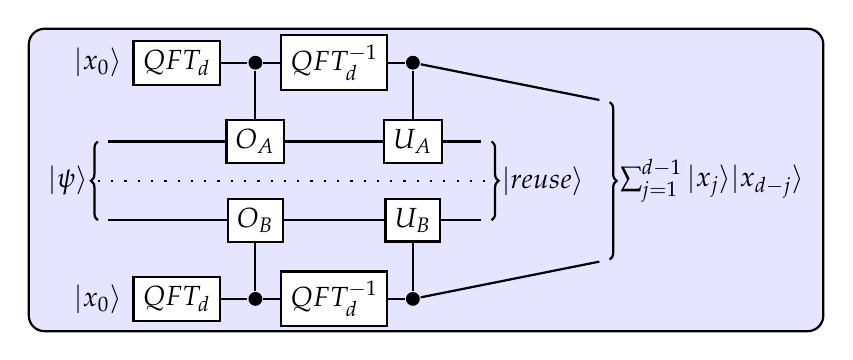
\begin{tikzpicture}[thick]
        %
        % `operator' will only be used by Hadamard (H) gates here.
        % `phase' is used for controlled phase gates (dots).
        % `surround' is used for the background box.
        \tikzstyle{operator} = [draw,fill=white,minimum size=1.5em] 
        \tikzstyle{phase} = [fill,shape=circle,minimum size=5pt,inner sep=0pt]
        \tikzstyle{surround} = [fill=blue!10,thick,draw=black,rounded corners=2mm]
        %
        % Bracket
        \draw[decorate,decoration={brace,mirror},thick] (0,-1) to
    	node[midway,left] (bracket1) {$\ket{\psi}$}
    	(0,-2);
        % Qubits
        \node at (0,0) (q1) {$\ket{x_0}$};
        \node at (0,-1) (q2) {};
        \node at (0,-2) (q3) {};
        \node at (0,-3) (q4) {$\ket{x_0}$};
        %
        % Column 1
        \node[operator] (op11) at (1,0) {$QFT_d$} edge [-] (q1);
        \node[operator] (op14) at (1,-3) {$QFT_d$} edge [-] (q4);
        %
        % Column 3
        \node[phase] (phase11) at (2,0) {} edge [-] (op11);
	\node[operator] (op22) at (2,-1) {$O_A$} edge [-] (q2);
	\node[operator] (op23) at (2, -2) {$O_B$} edge[-] (q3);
        \node[phase] (phase14) at (2,-3) {} edge [-] (op14);
        \draw[-] (phase11) -- (op22);
        \draw[-] (phase14) -- (op23);
        %
        % Column 4
        \node[operator] (op31) at (3,0) {$QFT_d^{-1}$} edge [-] (phase11);
        \node[operator] (op34) at (3,-3) {$QFT_d^{-1}$} edge [-] (phase14);
        %
        % Column 5
        \node[phase] (phase21) at (4,0) {} edge [-] (op31);
	\node[operator] (op42) at (4,-1) {$U_A$} edge [-] (op22);
	\node[operator] (op43) at (4, -2) {$U_B$} edge[-] (op23);
        \node[phase] (phase24) at (4,-3) {} edge [-] (op34);
        \draw[-] (phase21) -- (op42);
        \draw[-] (phase24) -- (op43);
        %
        % Column 6
        \node (end2) at (5,-1) {} edge [-] (op42);
        \node (end3) at (5,-2) {} edge [-] (op43);
        %
        % Bracket
        \draw[decorate,decoration={brace},thick] (5,-1) to
    	node[midway,right] (bracket) {$\ket{reuse}$}
    	(5,-2);
        %
        % Column 7
        \node (end1) at (6.5,-0.5) {} edge [-] (phase21);
        \node (end4) at (6.5,-2.5) {} edge [-] (phase24);
        % Dashed line
        \draw[loosely dotted] (0,-1.5) -- (5,-1.5);
        % Bracket
        \draw[decorate,decoration={brace},thick,] (6.5,-0.5) to
    	node[midway,right] (bracket2) {$\sum_{j=1}^{d-1}\ket{x_j}\ket{x_{d-j}}$}
    	(6.5,-2.5);
        %
        % Background Box
        \begin{pgfonlayer}{background} 
        \node[surround] (background) [fit = (q1) (op14) (bracket1)(bracket2)] {};
        \end{pgfonlayer}
        %
        \end{tikzpicture}
	\caption{The isometries $\Phi_{A,1} \x \Phi_{B,1}$.}
\end{figure}

The first isometry has the following steps:
\begin{enumerate}
	\item Append control register $\ket{x_0}_{A'}$ on Alice's side and $\ket{x_0}_{B'}$ on Bob's side;
	\item Apply Quantum Fourier Transform ($QFT_d$) to Alice and Bob's control registers;
	\item Apply Controlled-$O_{A/B}$ operations (i.e. if the control register is in state $\ket{x_k}_{A'/ B'}$, apply
	$O_{A/B}^k$.);
	\item Apply inverse Quantum Fourier Transform ($QFT_d^{-1}$) to the control registers;
	\item Apply Controlled-$U_{A/B}$ operations (i.e. If Alice's control register is in state $\ket{x_j}$, she applies
	$U_A^{\log_r (d-j)}$. If Bob's control register is in state $\ket{x_j}$, he applies $(U_B)^{\log_r j}$).
\end{enumerate}

\begin{figure}[H]
\center
        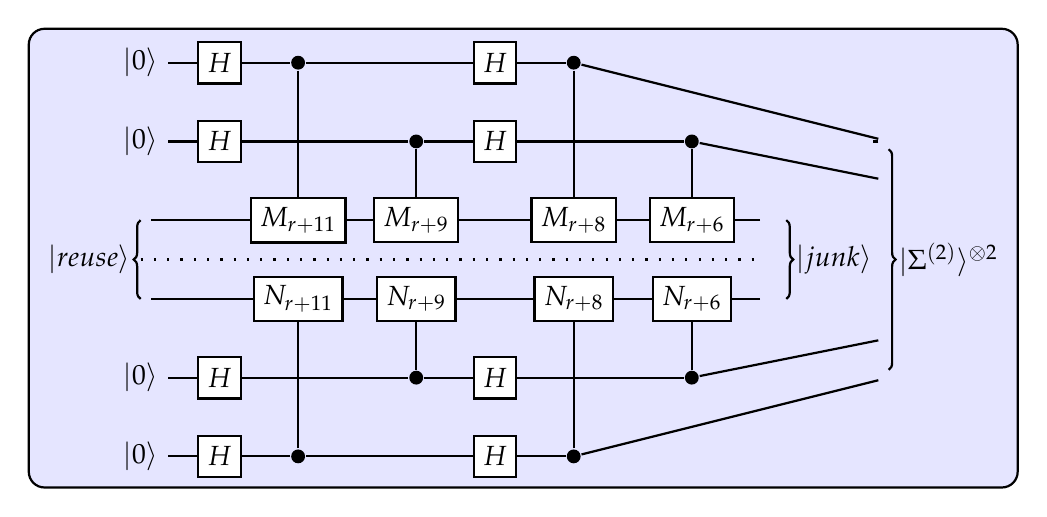
\begin{tikzpicture}[thick]
        %
        % `operator' will only be used by Hadamard (H) gates here.
        % `phase' is used for controlled phase gates (dots).
        % `surround' is used for the background box.
        \tikzstyle{operator} = [draw,fill=white,minimum size=1.5em] 
        \tikzstyle{phase} = [fill,shape=circle,minimum size=5pt,inner sep=0pt]
        \tikzstyle{surround} = [fill=blue!10,thick,draw=black,rounded corners=2mm]
        %
        % Bracket
        \draw[decorate,decoration={brace,mirror},thick] (0,-2) to
    	node[midway,left] (bracket1) {$\ket{reuse}$}
    	(0,-3);
        % Qubits
        \node at (0,0) (q1) {$\ket{0}$};
        \node at (0,-1) (q2) {$\ket{0}$};
        \node at (0,-2) (q3) {};
        \node at (0,-3) (q4) {};
        \node at (0,-4) (q5) {$\ket{0}$};
        \node at (0,-5) (q6) {$\ket{0}$};
        %
        % Column 1
        \node[operator] (op11) at (1,0) {$H$} edge [-] (q1);
        \node[operator] (op12) at (1,-1) {$H$} edge [-] (q2);
         \node[operator] (op15) at (1,-4) {$H$} edge [-] (q5);
        \node[operator] (op16) at (1,-5) {$H$} edge [-] (q6);
        %
        % Column 3
        \node[phase] (phase11) at (2,0) {} edge [-] (op11);
	\node[operator] (op23) at (2,-2) {$M_{r+11}$} edge [-] (q3);
	\node[operator] (op24) at (2, -3) {$N_{r+11}$} edge[-] (q4);
        \node[phase] (phase16) at (2,-5) {} edge [-] (op16);
        \draw[-] (phase11) -- (op23);
        \draw[-] (phase16) -- (op24);
        %
        % Column 4
        \node[phase] (phase12) at (3.5,-1) {} edge [-] (op12);
	\node[operator] (op33) at (3.5,-2) {$M_{r+9}$} edge [-] (op23);
	\node[operator] (op34) at (3.5, -3) {$N_{r+9}$} edge[-] (op24);
        \node[phase] (phase15) at (3.5,-4) {} edge [-] (op15);
        \draw[-] (phase12) -- (op33);
        \draw[-] (phase15) -- (op34);
        %
         % Column 5
        \node[operator] (op41) at (4.5,0) {$H$} edge [-] (phase11);
        \node[operator] (op42) at (4.5,-1) {$H$} edge [-] (phase12);
         \node[operator] (op45) at (4.5,-4) {$H$} edge [-] (phase15);
        \node[operator] (op46) at (4.5,-5) {$H$} edge [-] (phase16);
        %
        % Column 6
        \node[phase] (phase51) at (5.5,0) {} edge [-] (op41);
	\node[operator] (op53) at (5.5,-2) {$M_{r+8}$} edge [-] (op33);
	\node[operator] (op54) at (5.5, -3) {$N_{r+8}$} edge[-] (op34);
        \node[phase] (phase56) at (5.5,-5) {} edge [-] (op46);
        \draw[-] (phase51) -- (op53);
        \draw[-] (phase56) -- (op54);
        %
        % Column 7
        \node[phase] (phase62) at (7,-1) {} edge [-] (op42);
	\node[operator] (op63) at (7,-2) {$M_{r+6}$} edge [-] (op53);
	\node[operator] (op64) at (7, -3) {$N_{r+6}$} edge[-] (op54);
        \node[phase] (phase65) at (7,-4) {} edge [-] (op45);
        \draw[-] (phase62) -- (op63);
        \draw[-] (phase65) -- (op64);
        %
        % Bracket
        \node(end3) at (8, -2) {} edge [-] (op63);
        \node(end4) at (8, -3) {} edge [-] (op64);
        \draw[decorate,decoration={brace},thick] (8.2,-2) to
    	node[midway,right] (bracket) {$\ket{junk}$}
    	(8.2,-3);
        %
        % Column 7
        \node (end1) at (9.5,-1) {} edge [-] (phase51);
        \node(end2) at (9.5, -1.5) {} edge [-] (phase62);
       \node(end5) at (9.5, -3.5) {} edge [-] (phase65);
        \node (end6) at (9.5,-4) {} edge [-] (phase56);
        % Dashed line
        \draw[loosely dotted] (0,-2.5) -- (7.8,-2.5);
        \draw[solid] (end1) -- (9.3, -1);
        % Bracket
        \draw[decorate,decoration={brace},thick,] (9.5,-1.1) to
    	node[midway,right] (bracket2) {$\ket{\EPR{2}}^{\x 2}$}
    	(9.5,-3.9);
        %
        % Background Box
        \begin{pgfonlayer}{background} 
        \node[surround] (background) [fit = (q1) (op16) (bracket1)(bracket2)] {};
        \end{pgfonlayer}
        %
        \end{tikzpicture}
	\caption{The isometries $\Phi_{A,2} \x \Phi_{B,2}$.}
\end{figure}

The second isometry is the standard isometry used in the self-testing result of the Magic Square game \cite{wu2016}.
The only thing to note is that the state $\ket{reuse}$, which is on the same Hilbert space as $\ket{\psi}$ and produced by $\Phi_{A,1} \x \Phi_{B,1}$, is the input state to $\Phi_{A,2} \x \Phi_{B,2}$. In this sense, our isometry is a $2$-step sequential procedure.

%We first list the key relations needed for $\Phi_{A,1} \x \Phi_{B,1}$ to work.
%\begin{align}
%	&\ket{\psi} \appd{O(d^{5/4} r^{d/2} r^{1/4} \ep^{1/8})}\ket{\psi'} = \sum_{j=1}^{d-1} (U_A\ct U_B\ct)^{\log_r j} \ket{\psi_1},\\
%	&O_A(U_A\ct)^{\log_r j} \ket{\psi_1} \appd{O(\sd r^j \sr \qe)}\omega_d^{-r^j}  (U_A\ct)^j \ket{\psi_1}\\
%	&O_B(U_A\ct)^{\log_r j} \ket{\psi_1} \appd{O(\sd r^j \sr \qe)}\omega_d^{r^j}  (U_A\ct)^j \ket{\psi_1}.
%\end{align}
%The second isometry just requires properties of the Magic Square game, especially, the commutation relations in \cref{prop:lct_comm}.


\begin{proof}[Proof of \cref{thm:self-test}]
The proof takes two steps. 
We first show that 
\begin{align}
	\Phi_{A,1}\x\Phi_{B,1}(\ket{\psi}) \appd{O(d^{5/2} r^{d+1/2} \ep^{1/8})} \sqrt{d-1}\ket{\psi_1} \x \frac{1}{\sqrt{d-1}}\sum_{j=1}^{d-1} \ket{x_{d-j}}_{A'}\ket{x_j}_{B'}.
\end{align}
Then we show that there exists a state $\ket{junk}$ such that  
\begin{align}
\label{eq:phi2_result}
\Phi_{A,2} \x \Phi_{B,2} (\sqrt{d-1}\ket{\psi_1}) \appd{O(r\se)} \ket{junk} \x \ket{\EPR{2}}^{\x 2}.
\end{align}
Combining the two equations above we get that 
\begin{align*}
	&\quad\Phi_{A,2} \x \Phi_{B,2}( \Phi_{A,1} \x \Phi_{B,1} (\ket{\psi})) \\
	&\appd{O(d^{5/2} \sr \ep^{1/8})} \Phi_{A,2} \x \Phi_{B,2}(\sqrt{d-1} \ket{\psi_1}) \x\frac{1}{\sqrt{d-1}}\sum_{j=1}^{d-1} \ket{x_{d-j}}_{A'}\ket{x_j}_{B'} \\
	&\appd{O(r\se)} \ket{junk} \x \ket{\EPR{2}}^{\x 2} \x\frac{1}{\sqrt{d-1}}\sum_{j=1}^{d-1} \ket{x_{d-j}}_{A'}\ket{x_j}_{B'},
\end{align*}
where we use the fact that $\Phi_{A,2}\x \Phi_{B,2}$ only acts on the state $\ket{\psi_1}$.

\Cref{lm:decomp_psi} implies that $ \Phi_{A,1} \x \Phi_{B,1} (\ket{\psi}) \appd{O(d r^{d/2 +1/4} \ep^{1/8})}  \Phi_{A,1} \x \Phi_{B,1} (\ket{\psi'})$,  
so we focus on how the isometry evolves $\ket{\psi'}$.
The evolution is summarized below.
	\begin{align*}
		& \sum_{j=1}^{d-1} (U_A\ct U_B\ct)^{\log_r j} \ket{\psi_1} \ket{x_0}_{A'}\ket{x_0}_{B'}\\
		\xrightarrow[]{QFT_d}& \frac{1}{d}\sum_{k_1,k_2 = 0}^{d-1} \sum_{j=1}^{d-1} (U_A\ct U_B\ct)^{\log_r j}  \ket{\psi_1}\ket{x_{k_1}}_{A'}\ket{x_{k_2}}_{B'}\\
		\xrightarrow[]{\text{Controlled-}O_{A/B}}& \frac{1}{d}\sum_{k_1,k_2 = 0}^{d-1} \sum_{j=1}^{d-1} O_A^{k_1}(U_A\ct)^{\log_r j} O_B^{k_2}(U_B\ct)^{\log_r j}
		\ket{\psi_1} \ket{x_{k_1}}_{A'}\ket{x_{k_2}}_{B'}\\
		\appd{O(d^{5/2} r^{d} \sr \qe)}&\frac{1}{d} \sum_{k_1,k_2 = 0}^{d-1} \sum_{j=1}^{d-1} (U_A\ct U_B\ct)^{\log_r j}\omega_d^{(k_2-k_1)j}\ket{\psi_1} \ket{x_{k_1}}_{A'}\ket{x_{k_2}}_{B'}\\
		\xrightarrow[]{QFT_d^{-1}} &\frac{1}{d^2}\sum_{l_1,l_2 = 0}^{d-1}\sum_{k_1,k_2 = 0}^{d-1}\sum_{j=1}^{d-1} (U_A\ct U_B\ct)^{\log_r j} 
		\omega_d^{k_1(d-j-l_1)}\omega_d^{k_2(j-l_2)}\ket{\psi_1} \ket{x_{l_1}}_{A'}\ket{x_{l_2}}_{B'}\\
		= &\sum_{j=1}^{d-1}(U_A\ct U_B\ct)^{\log_r j} \ket{\psi_1} \ket{x_{d-j}}_{A'}\ket{x_j}_{B'} \\
		\xrightarrow[]{\text{Controlled-}U_{A/B}}& \sum_{j=1}^{d-1} U_A^{\log_r j} (U_A\ct)^{\log_r j} U_B^{\log_r j} (U_B\ct)^{\log_r j} \ket{\psi_1} \ket{x_{d-j}}_{A'}\ket{x_j}_{B'}\\
		=&\ket{\psi_1} \x \sum_{j=1}^{d-1} \ket{x_{d-j}}_{A'}\ket{x_j}_{B'}.
	\end{align*}
When we analyze the effect of the controlled-$O_{A/B}$, we applied \cref{eq:A_omega,eq:B_omega} repeatedly.
In summary, we have shown that
\begin{align}
	\Phi_{A,1}\x\Phi_{B,1}(\ket{\psi}) \appd{O(d^{5/2} r^{d+1/2} \ep^{1/8})} \sqrt{d-1} \ket{\psi_1} \x \frac{1}{\sqrt{d-1}}\sum_{j=1}^{d-1} \ket{x_{d-j}}_{A'}\ket{x_j}_{B'},
\end{align}
where we use the fact that $O(d^{5/2} r^{d+1/2} \ep^{1/8})$ dominates both $O(d r^{d/2+1/4} \ep^{1/8})$ and 
$O(d^{5/2} r^{d+1/2} \qe)$.
Since $\norm{\ket{\psi_1}}^2 \appd{O(r \se)} 1/(d-1)$, we know $ \sqrt{d-1} \norm{\ket{\psi_1}} \appd{O(\sd \sr\qe)} 1$.

To prove \cref{eq:phi2_result}, we first
recall that 
$\ket{\psi_1} 
	=\frac{1}{2} (M_{\nr+1}^0 + iM_{\nr+2}M_{\nr+1}^1 - iM_{\nr+2}M_{\nr+1}^0 + M_{\nr+1}^1) \ket{\psi}.
$
The other observation that we need is that 
\begin{align*}
	&\Phi_{A,2} \x \Phi_{B,2} (\ket{\psi_1})  \\
	= &\frac{1}{16} \sum_{\ba, \bb \in\{0,1\}^4}
	M(f_0)^{a(4)}N(f_0)^{b(4)}M(f_2)^{a(3)}N(f_2)^{b(3)}M(g_0)^{a(2)}N(g_0)^{b(2)}M(g_2)^{a(1)}N(g_2)^{b(1)}
	\ket{\psi_1} \ket{\ba}_{A''} \ket{\bb}_{B''}
\end{align*}
For simplicity we define $M^{\ba} := M(f_0)^{a(4)}M(f_2)^{a(3)}M(g_0)^{a(2)}M(g_2)^{a(1)}$ and
$N^{\bb} := N(f_0)^{b(4)}N(f_2)^{b(3)}N(g_0)^{b(2)}N(g_2)^{b(1)} $.
We would like to show that 
\begin{align}
\label{eq:mua_comm}
M^{\ba} \ket{\psi_1} \appd{O(r\se)} \frac{1}{2} (M_{\nr+1}^0 + iM_{\nr+2}M_{\nr+1}^1 - iM_{\nr+2}M_{\nr+1}^0 + M_{\nr+1}^1)
M^{\ba} \ket{\psi},
\end{align}
for all $\ba \in \{0,1\}^4$,
%which implies that 
%\begin{align*}
%	\Phi_{A,2} \x &\Phi_{B,2} (\ket{\psi_1}) \appd{O(r\se)} \\
%	&\frac{1}{2} (M_{\nr+1}^0 + iM_{\nr+2}M_{\nr+1}^1 - iM_{\nr+2}M_{\nr+1}^0 + M_{\nr+1}^1)(\Phi_{A,2} \x \Phi_{B,2}(\ket{\psi}))
%\end{align*}
%because $N^{\ub}$ commutes with $\frac{1}{2} (M_{\nr+1}^0 + iM_{\nr+2}M_{\nr+1}^1 - iM_{\nr+2}M_{\nr+1}^0 + M_{\nr+1}^1)$
%for all $\ub \in \{0,1\}^4$.
which can be justified by \cref{prop:rel_comm}.
We show how to apply \cref{prop:rel_comm} to commute $M(g_2)^{a(1)}$ through 
$\frac{1}{2} (M_{\nr+1}^0 + iM_{\nr+2}M_{\nr+1}^1 - iM_{\nr+2}M_{\nr+1}^0 + M_{\nr+1}^1)$ and then similar process can be repeated for $M(g_0)^{a(2)}, M(f_2)^{a(3)}$ and $M(f_0)^{a(4)}$,
\begin{align*}
	&\quad M(g_2)^{a(1)} \frac{1}{2} (M_{\nr+1}^0 + iM_{\nr+2}M_{\nr+1}^1 - iM_{\nr+2}M_{\nr+1}^0 + M_{\nr+1}^1) \ket{\psi} \\
	&\appd{O(\sr\se)} \frac{1}{2}[ (M_{\nr+1}^0+M_{\nr+1}^1) M(g_2)^{a(1)} -i M(g_2)^{a(1)} M_{\nr+2}N_{\nr+1}] \ket{\psi} \\
	&\appd{O(\sr\se)} \frac{1}{2} [(M_{\nr+1}^0+M_{\nr+1}^1) M(g_2)^{a(1)} - iM_{\nr+2}M(g_2)^{a(1)} N_{\nr+1}] \ket{\psi} \\
	&\appd{O(\sr\se)}\frac{1}{2} [(M_{\nr+1}^0+M_{\nr+1}^1) M(g_2)^{a(1)} - iM_{\nr+2}M(g_2)^{a(1)} M_{\nr+1}] \ket{\psi} \\
	&\appd{O(\sr\se)}\frac{1}{2} [(M_{\nr+1}^0+M_{\nr+1}^1) M(g_2)^{a(1)} - iM_{\nr+2}M_{\nr+1}M(g_2)^{a(1)} ] \ket{\psi}.
\end{align*}
In summary, we have 
\begin{align}
	M^{\ba} N^{\bb} \ket{\psi_1} \appd{O(\sr\se)} \frac{1}{2} (M_{\nr+1}^0 + iM_{\nr+2}M_{\nr+1}^1 - iM_{\nr+2}M_{\nr+1}^0 + M_{\nr+1}^1)M^{\ba}N^{\bb} \ket{\psi}
\end{align}
for all $\ba, \bb \in \{0,1\}^4$, which implies that 
\begin{align*}
	\Phi_{A,2} \x& \Phi_{B,2}(\ket{\psi_1}) \appd{O(\sr\se)}\\
	 &\frac{1}{2} (M_{\nr+1}^0 + iM_{\nr+2}M_{\nr+1}^1 - iM_{\nr+2}M_{\nr+1}^0 + M_{\nr+1}^1)(\Phi_{A,2}\x\Phi_{B,2} (\ket{\psi}).
\end{align*}
At this point we can apply Lemma C.$1$ of \cite{wu2016} to $\Phi_{A,2}\x\Phi_{B,2} (\ket{\psi})$ and conclude that 
\begin{align}
	\Phi_{A,2} \x \Phi_{B,2}(\sqrt{d-1} \ket{\psi_1}) \appd{O(\sd \sr \se)} \ket{junk} \x \ket{\EPR{2}}^{\x 2},
\end{align} 
for some state $\ket{junk}$ whose norm can be deduced from the norm of $\ket{\psi_1}$.

In the rest of the proof, we only show how $\Phi_{A,1} \x \Phi_{B,1}$ acts on $O_A\ket{\psi}$ and $U_A\ket{\psi}$.

If the initial state is $O_A\ket{\psi}$, we first use the fact that 
$ \Phi_{A,1} \x \Phi_{B,1} (O_A\ket{\psi}) \appd{O(d^{5/4} r^{d/2+1/4} \ep^{1/8})}  \Phi_{A,1} \x \Phi_{B,1} (O_A\ket{\psi'})$, 
and then we calculate $\Phi_{A,1} \x \Phi_{B,1} (O_A\ket{\psi'})$ as
\begin{align*}
	O_A \ket{\psi'} \ket{x_0}_{A'}\ket{x_0}_{B'} =&  
		\sum_{j=1}^{d-1} O_A(U_A\ct U_B\ct)^{\log_r j}\ket{\psi_1}\ket{x_0}_{A'}\ket{x_0}_{B'}\\
		\appd{O(\sd r^{d+1/2} \ep^{1/4})}&\sum_{j=1}^{d-1}(U_A\ct U_B\ct)^{\log_r j} \omega_d^{-j} \ket{\psi_1} \ket{x_0}_{A'}\ket{x_0}_{B'}\\
		\xrightarrow[]{QFT_d} &\frac{1}{d}\sum_{j=1}^{d-1} \sum_{k_1,k_2 = 0}^{d-1}(U_A\ct U_B\ct)^{\log_r j} \omega_d^{-j} 
		\ket{\psi_1}\ket{x_{k_1}}_{A'}\ket{x_{k_2}}_{B'}\\
		\xrightarrow[]{\text{Controlled-}O_{A/B}}&\frac{1}{d}\sum_{j=1}^{d-1}\sum_{k_1,k_2 = 0}^{d-1} 
		 O_A^{k_1}(U_A\ct)^{\log_r j} O_B^{k_2}(U_B\ct)^{\log_r j} \omega_d^{-j} \ket{\psi_1} 
		 \ket{x_{k_1}}_{A'}\ket{x_{k_2}}_{B'}\\
		\appd{O(d^{5/2} r^{d+1/2}  \ep^{1/4})}& \frac{1}{d}\sum_{k_1,k_2 = 0}^{d-1} \sum_{j=1}^{d-1} (U_A\ct U_B\ct)^{\log_r j}
		\omega_d^{-j}\omega_d^{(k_2-k_1)j}\ket{\psi_1}
		 \ket{x_{k_1}}_{A'}\ket{x_{k_2}}_{B'}\\
		\xrightarrow[]{QFT_d^{-1}}& \sum_{j=1}^{d-1}  (U_A\ct U_B\ct)^{\log_r j}  
		\omega_d^{d-j}\ket{\psi_1} \ket{x_{d-j}}_{A'}\ket{x_j}_{B'}\\
		\xrightarrow[]{\text{Controlled-}U_{A/B}}&   \sqrt{d-1} \ket{\psi_1} \x  
		\frac{1}{\sqrt{d-1}}\sum_{j=1}^{d-1} \omega_d^{d-j}\ket{x_{d-j}}_{A'}\ket{x_j}_{B'}.
\end{align*}
The analysis for $\Phi_{A,1} \x\Phi_{B,1} (O_B \ket{\psi})$ is very similar.

If the initial state is $U_A\ket{\psi}$, we first use the fact that 
$ \Phi_{A,1} \x \Phi_{B,1} (U_A\ket{\psi}) \appd{O(d^{5/4}r^{d/2+1/4} \ep^{1/8})}  \Phi_{A,1} \x \Phi_{B,1} (U_A\ket{\psi'})$, 
and then we calculate $\Phi_{A,1} \x \Phi_{B,1} (U_A\ket{\psi'})$.
\begin{align*}
	U_A \ket{\psi'} \ket{x_0}_{A'}\ket{x_0}_{B'} =&  
		\sum_{j=1}^{d-1} U_A(U_A\ct U_B\ct)^{\log_r j}\ket{\psi_1} \ket{x_0}_{A'}\ket{x_0}_{B'}\\
		=&\sum_{j=1}^{d-1}(U_A\ct)^{\log_r j-1}  (U_B\ct)^{\log_r j} \ket{\psi_1} \ket{x_0}_{A'}\ket{x_0}_{B'}\\
		\xrightarrow[]{QFT_d} &\frac{1}{d}\sum_{j=1}^{d-1} \sum_{k_1,k_2 = 0}^{d-1}(U_A\ct)^{\log_r j-1} (U_B\ct)^{\log_r j} \ket{\psi_1}  \ket{x_{k_1}}_{A'}\ket{x_{k_2}}_{B'}\\
		\xrightarrow[]{\text{Controlled-}O_{A/B}}&\frac{1}{d}\sum_{j=1}^{d-1}\sum_{k_1,k_2 = 0}^{d-1} 
		 O_A^{k_1}(U_A\ct)^{\log_r j-1} O_B^{k_2}(U_B\ct)^{\log_r j} \ket{\psi_1} 
		 \ket{x_{k_1}}_{A'}\ket{x_{k_2}}_{B'}\\
		\appd{O(d^{5/2} r^{d+1/2} \qe)}& \frac{1}{d}\sum_{k_1,k_2 = 0}^{d-1} \sum_{j=1}^{d-1} (U_A\ct)^{\log_r j-1} (U_B\ct)^{\log_r j}
		\omega_d^{k_2j-k_1jr^{-1}}\ket{\psi_1}
		 \ket{x_{k_1}}_{A'}\ket{x_{k_2}}_{B'}\\
		\xrightarrow[]{QFT_d^{-1}}& \sum_{j=1}^{d-1}  (U_A\ct)^{\log_r j-1} (U_B\ct)^{\log_r j}  
		\ket{\psi_1} \ket{x_{(d-j)r^{-1}}}_{A'}\ket{x_j}_{B'}\\
		\xrightarrow[]{\text{Controlled-}U_{A/B}}& \sqrt{d-1} \ket{\psi_1} \x  
		\frac{1}{\sqrt{d-1}} \sum_{j=1}^{d-1} \ket{x_{(d-j)r^{-1}}}_{A'}\ket{x_j}_{B'},
\end{align*}
where we use the fact that $(d-j)r^{-1} \equiv d -jr^{-1} \pmod{d}$.
The analysis for $\Phi_{A,1} \x\Phi_{B,1} (U_B \ket{\psi})$ is very similar.
\end{proof}

%%-----------------------------------------------------------------
%\subsection{Self-test}
%%-----------------------------------------------------------------
%\hl{This subsection needs to be formalized.}
%We give a formal version of \cref{thm:pr_2} first and then prove it.
%\begin{theorem}
%\label{thm:selftest}
%	If a quantum strategy using the shared state $\ket{\psi}$ achieves the ideal 2-party correlation $C(\dr{r})$ where $d$ is an odd
%	prime number with primitive root $r \in \{2,3,5\}$, then there exist local isometries $\Phi_A$ and $\Phi_B$, and a state $\ket{junk}$ such 
%	that $\Phi_A\x\Phi_B \ket{\psi} = \ket{\EPR{d-1}} \x \ket{junk}$.
%\end{theorem}
%\begin{proof}
%Suppose Alice and Bob achieve the optimal correlation with the quantum strategy $(\ket{\psi}, \{A_x\}, \{B_y\})$
%for all $x,y \in \calX \times \calY$ .
%The observables $A_x$ and $B_y$ and the shared state $\ket{\psi}$ shall not be confused with the ones used in the optimal strategy.
%By Lemma~$4.3$ of Ref.~\cite{coladan2017}, we can extract an operator solution from the perfect winning strategy 
%of the linear system game $\LS_r$. 
%For each variable $\{ x_i \}_{i=1}^{n_r}$, Alice and Bob has operators $A_i$ and $B_i$ respectively.
%The condition that they agree with assignment to variables means that 
%\begin{align}
%	\bra{\psi} A_i \otimes \overline{B_i} \ket{\psi} = 1 \Rightarrow A_i \otimes \overline{B_i} \ket{\psi} = \ket{\psi}
%	\text{ for } 1 \leq i \leq n_r
%\end{align}
%and the condition that Alice's assignments satisfy the constraint means that 
%\begin{align}
%	\Tr(\rho_A \Pi_{j: H(i,j) \neq 0} A_j) = \Tr(\rho_A) \text{ for all } 1 \leq i \leq m_r
%\end{align}
%where $\rho_A =  \Tr_B(\ketbra{\psi}{\psi})$. 
%Similarly we define $\rho_B = \Tr_A(\ketbra{\psi}{\psi})$.
%For any $\ket{v} \in \supp(\rho_A)$,
%we have 
%\begin{align}
%\Pi_{j:H(i,j) \neq 0} A_j \ket{v} = \ket{v} \text{ for all } 1 \leq i \leq m_r.
%\end{align}
%Since the relation $uxu^{-1} = x^r$, where $r$ is the primitive root of $d$, is embedded in this linear system game, we know
%\begin{align}
%	A_3A_4 A_1A_2 (A_3A_4)^\dagger \ket{v}= (A_1A_2)^r \ket{v} \text{ for all } \ket{v} \in \supp(\rho_A).
%\end{align}
%For simplicity, we define $X_A = A_1A_2$ and $U_A=A_3A_4$ such that
%the condition is equivalent to
%\begin{align}
%	\label{eq:ux_relation}
%	U_AX_AU_A^\dagger \ket{v} = X_A^r \ket{v} \text{ for all } \ket{v} \in \supp(\rho_A).
%\end{align}
%We will come back to the implication of this condition later.
%
%Suppose $A_{m_r+1} = A_\ast^0- A_\ast^\perp = \Pi_{V_A} - \Pi_{V_A^\perp}$m, where $V_A$ is a
%$2m$-dimensional vector space and $\Pi_{V_A}$ is the projector onto it. The reason why it has dimension $2m$
%will be clear shortly. On Bob's side, we also have $B_{n_r+1} = B_\ast^0- B_\ast^\perp = \Pi_{V_B} - \Pi_{V_B^\perp}$.
%Recall that from the extended weighted CHSH test, we know
%\begin{align}
%	A_\ast^0 \ket{\psi} = B_\ast^0 \ket{\psi} = A_\ast^0 \x B_\ast^0 \ket{\psi},
%\end{align}
%which implies that with an appropriate change of basis, we can get $V_A = V_B$, so in the rest of the proof
%we drop the subscript of $V$.
%By \cref{lm:chsh_comp} and \cref{prop:2d-subspace}, we know $V$ consists of $\omega_d$-eigenvectors and $\omega_d^{-1}$ eigenvectors of 
%$X_A$, so we can write 
%\begin{align}
%	\Pi_{V} = \Pi_{V_1} + \Pi_{V_{d-1}},
%\end{align}
%where $\Pi_{V_{1}}$ is the projector onto the $\omega_d$-eigenspace of $X_A$ and $\Pi_{V_{d-1}}$ is the projector 
%onto the $\omega_d^{-1}$-eigenspace of $X_A$.
%\hl{Here what we need is that $\Pi_{V_1,A} \ket{\psi} = \Pi_{V_{d-1},B} \ket{\psi} = \Pi_{V_1,A}\Pi_{V_{d-1},B}\ket{\psi}$
%and $\Pi_{V_1,B} \ket{\psi} = \Pi_{V_{d-1},A} \ket{\psi} = \Pi_{V_1,B}\Pi_{V_{d-1},A}\ket{\psi}$.
%This is not proved because $\Pi_{V_1}$ and $\Pi_{V_{d-1}}$ are not in the strategy.}
%Suppose $\ket{x_{1}} \in V_{1}$, then $X_A \ket{x_{1}} = \omega_d \ket{x_{1}}$.
%By \cref{eq:ux_relation} we can calculate that
%\begin{align}
%\label{eq:ladder}
% X_AU_A^\dagger \ket{x_{1}} = U_A^\dagger X_A^r \ket{x_{1}} = \omega_d^r U_A^\dagger \ket{x_{1}},
%\end{align}
%so $U_A^\dagger \ket{x_{1}}$ is an eigenvector of $X_A$ with eigenvalue $\omega_d^r$.
%By induction, we know $X_A (U_A^\dagger)^i \ket{x_{1}} = \omega_d^{r^i} (U_A^\dagger)^i\ket{x_{1}}$. 
%From the set $\{(U_A^\dagger)^i \Pi_{V_1} (U_A)^i \}_{i=0}^{d-2}$, we can identify $\Pi_{V_i}$ for $i = 1 \dots  d-1$
%such that $\Pi_{V_i}$ is the projector onto the $\omega_d^i$-eigenspace of $X_A$,
%\hl{Actually, we are not sure about the containment between $\supp((U_A\ct)^{\log_r(d-1)} \Pi_{V_1} U_A^{\log_r(d-1)})$ and 
%$\supp(\Pi_{V_{d-1}})$, so we cannot say that $\Pi_{V_{d-1}} = (U_A\ct)^{\log_r(d-1)} \Pi_{V_1} U_A^{\log_r(d-1)}$.}
%and 
%\begin{align}
% \cup_{i \in [d-1]+1} V_i \subset \supp(\rho_A).
%\end{align}
%Since unitary transformation does not change the rank of a matrix, we know $\rank(\Pi_{V_1}) = \rank(\Pi_{V_{i}}) =N$
%for $ i =1 \dots d-1$.
%We pick a basis for $V_1$ such that 
%\begin{align}
%	\Pi_{V_1} =  \sum_{j=1}^m \ketbra{x_{1,j}}{x_{1,j}},
%\end{align}
%then we can construct 
%\begin{align}
% \Pi_{V_i} = \sum_{j=1}^m \ketbra{x_{i,j}}{x_{i,j}},
%\end{align}
%where $\ket{x_{i,j}} = (U\ct)^{k_i} \ket{x_{1,j}}$ for $r^{k_i} \equiv i \pmod{d}$ and $1 \leq j \leq m$.
%By \cref{eq:ux_relation} we also know that $U_A \ket{x_{i,j}} = \ket{x_{i/2,j}}$ for $i = 1,2 \dots d-1$.
%In order to apply \cref{lm:ux_independ}, we construct $m$ subspaces $\{W_j\}_{j=1}^m$ where 
%\begin{align}
%	W_j = \spn( \{ \ket{x_{i,j}} \}_{i=1}^{d-1} )
%\end{align}
%The subspace $W_j$ is orthogonal to $W_{j'}$ for $j \neq j'$, and
%$U_A$ and $X_A$ satisfy the condition of \cref{lm:ux_independ} when their actions are 
%restricted to each $W_j$.
%Similar argument also applies to operator $X_B$ and $U_B$ on Bob's side.


%With an appropriate change of basis, we 
%assume that $\ket{\psi} = \vc(\tau)$ for some $\tau \in L(\supp(\rho_A))$
%The consistency condition is equivalent to
%\begin{align}
%\label{eq:con_tau}
%	A_i \tau B_i^\dagger = \tau.
%\end{align}
%Substituting $i=1,2$ into \cref{eq:con_tau}, we get 
%\begin{align}
%	X_A \tau X_A^\dagger = A_1A_2\tau B_2^\dagger B_1^\dagger = A_1\tau B_1^\dagger = \tau.
%\end{align}
%Similar argument gives us that 
%\begin{align}
%	U_A \tau U_A^\dagger = \tau.
%\end{align}
%Then we can conclude that for any $k \in \{0,1 \dots d-2\}$ and $l \in \{1,2\dots d-1\}$
%\begin{align}
%	U_A^kX_A^l \tau (U_A^kX_A^l)^\dagger = \tau.
%\end{align}
%Let $\Pi_{W_j}$ be the projector onto $W_j$. 
%By \cref{lm:ux_independ}, $\Pi_{W_j} \tau \Pi_{W_j}$ commutes with all the $(d-1) \times (d-1)$ matrices, which means that 
%\begin{align}
%	\label{eq:d-1}
%	\Pi_{W_j} \tau \Pi_{W_j}  = c_j \1_{W_j} \text{ for } j = 1\dots m.
%\end{align}
%In the vector form, we know
%\begin{align}
%	\sum_{j =1}^N \Pi_{W_j} \ket{\psi} =\sum_{i=1}^{d-1} \sum_{j=1}^m c_j \ket{x_{i,j}}\ket{x_{i,j}}. 
%\end{align}
%Recalling the fact that 
%\begin{align}
%\norm{ \Pi_{V_1} + \Pi_{V_{d-1}} \ket{\psi}}^2 = \norm{\Pi_{V_1} \ket{\psi}}^2 + \norm{\Pi_{V_{d-1}} \ket{\psi}}^2 = \frac{2}{d-1},
% \end{align}
% it means that 
% \begin{align}
% 	2 \sum_{j=1}^m \norm{c_j}^2 = \frac{2}{d-1}.
% \end{align}
% Then we can calculate the norm of $\sum_{j =1}^m \Pi_{W_j} \ket{\psi}$, which is
% \begin{align}
% \norm{\sum_{j =1}^m \Pi_{W_j} \ket{\psi}}^2 = \sum_{i=1}^{d-1} \sum_{j=1}^m \norm{c_j}^2 = 1 = \norm{\ket{\psi}}^2.
% \end{align}
% We can conclude that $\supp{\rho_A} = \cup_{i=1}^{d-1} V_i$ and 
% \begin{align}
% 	\ket{\psi} = \sum_{i=1}^{d-1}\sum_{j=1}^m c_j \ket{x_{i,j}}\ket{x_{i,j}}.
% \end{align}
% 
%The last step is to construct the local isometries $\Phi_A$ and $\Phi_B$ that can produce $\ket{\EPR{d-1}}$ from $\ket{\psi}$.
%To help understanding, we draw a diagram to demonstrate the isometry first and then show
%how this isometry works.
%\begin{figure}[H]
%\center
%        \begin{tikzpicture}[thick]
%        %
%        % `operator' will only be used by Hadamard (H) gates here.
%        % `phase' is used for controlled phase gates (dots).
%        % `surround' is used for the background box.
%        \tikzstyle{operator} = [draw,fill=white,minimum size=1.5em] 
%        \tikzstyle{phase} = [fill,shape=circle,minimum size=5pt,inner sep=0pt]
%        \tikzstyle{surround} = [fill=blue!10,thick,draw=black,rounded corners=2mm]
%        %
%        % Bracket
%        \draw[decorate,decoration={brace,mirror},thick] (0,-1) to
%    	node[midway,left] (bracket1) {$\ket{\psi}$}
%    	(0,-2);
%        % Qubits
%        \node at (0,0) (q1) {$\ket{0}$};
%        \node at (0,-1) (q2) {};
%        \node at (0,-2) (q3) {};
%        \node at (0,-3) (q4) {$\ket{0}$};
%        %
%        % Column 1
%        \node[operator] (op11) at (1,0) {$QFT_d$} edge [-] (q1);
%        \node[operator] (op14) at (1,-3) {$QFT_d$} edge [-] (q4);
%        %
%        % Column 3
%        \node[phase] (phase11) at (2,0) {} edge [-] (op11);
%	\node[operator] (op22) at (2,-1) {$X_A$} edge [-] (q2);
%	\node[operator] (op23) at (2, -2) {$X_B$} edge[-] (q3);
%        \node[phase] (phase14) at (2,-3) {} edge [-] (op14);
%        \draw[-] (phase11) -- (op22);
%        \draw[-] (phase14) -- (op23);
%        %
%        % Column 4
%        \node[operator] (op31) at (3,0) {$QFT_d^{-1}$} edge [-] (phase11);
%        \node[operator] (op34) at (3,-3) {$QFT_d^{-1}$} edge [-] (phase14);
%        %
%        % Column 5
%        \node[phase] (phase21) at (4,0) {} edge [-] (op31);
%	\node[operator] (op42) at (4,-1) {$U_A$} edge [-] (op22);
%	\node[operator] (op43) at (4, -2) {$U_B$} edge[-] (op23);
%        \node[phase] (phase24) at (4,-3) {} edge [-] (op34);
%        \draw[-] (phase21) -- (op42);
%        \draw[-] (phase24) -- (op43);
%        %
%        % Column 6
%        \node (end2) at (5,-1) {} edge [-] (op42);
%        \node (end3) at (5,-2) {} edge [-] (op43);
%        %
%        % Bracket
%        \draw[decorate,decoration={brace},thick] (5,-1) to
%    	node[midway,right] (bracket) {$\ket{junk}$}
%    	(5,-2);
%        %
%        % Column 7
%        \node (end1) at (6.5,-0.5) {} edge [-] (phase21);
%        \node (end4) at (6.5,-2.5) {} edge [-] (phase24);
%        % Dashed line
%        \draw[loosely dotted] (0,-1.5) -- (5,-1.5);
%        % Bracket
%        \draw[decorate,decoration={brace},thick,] (6.5,-0.5) to
%    	node[midway,right] (bracket2) {$\ket{\EPR{d-1}}$}
%    	(6.5,-2.5);
%        %
%        % Background Box
%        \begin{pgfonlayer}{background} 
%        \node[surround] (background) [fit = (q1) (op14) (bracket1)(bracket2)] {};
%        \end{pgfonlayer}
%        %
%        \end{tikzpicture}
%	\caption{The isometries $\Phi_A$ and $\Phi_B$.}
%\end{figure}
%The isometry maps the state $\ket{\psi}$ in the following steps:
%\begin{enumerate}
%	\item Append $\ket{0}_A$ on Alice's side and $\ket{0}_B$ on Bob's side as control registers, and
%	the state becomes $\ket{\psi} \ket{0}_A \ket{0}_B$;
%	\item Apply $QFT_d$ to the control registers, and the state becomes
%	\begin{align}
%		\frac{1}{d} \sum_{k_1,k_2 =0}^{d-1} \ket{\psi} \ket{k_1}_A \ket{k_2}_B;
%	\end{align}
%	\item Apply $X_A^{k_1}$ to Alice's share of $\ket{\psi}$ and $X_B^{k_2}$ to Bob's share controlled
%	by the control registers, and the state becomes
%	\begin{align}
%		&\frac{1}{d} \sum_{k_1,k_2 =0}^{d-1}X_A^{k_1} X_B^{k_2}\ket{\psi} \ket{k_1}_A \ket{k_2}_B\\
%		=&\frac{1}{d} \sum_{k_1,k_2 =0}^{d-1} \sum_{i=1}^{d-1}\sum_{j=1}^m c_j X_A^{k_1}\ket{x_{i,j}}_A X_B^{k_2}\ket{x_{i,j}}_B
%		\ket{k_1}_A \ket{k_2}_B\\
%		=&\frac{1}{d} \sum_{k_1,k_2 =0}^{d-1} \sum_{i=1}^{d-1}\sum_{j=1}^m c_j \omega_d^{k_1i+k_2i} \ket{x_{i,j}}_A\ket{x_{i,j}}_B
%		\ket{k_1}_A \ket{k_2}_B;
%	\end{align}
%	\item Apply $QFT_d^{-1}$ to the control registers, and the state becomes
%	\begin{align}
%		&\frac{1}{d^2} \sum_{l_1,l_2 =0}^{d-1}\sum_{i=1}^{d-1}\sum_{j=1}^m c_j \omega_d^{k_1(i-l_1)+k_2(i-l_2)} \ket{x_{i,j}}_A\ket{x_{i,j}}_B
%		\ket{l_1}_A \ket{l_2}_B\\
%		=& \sum_{i=1}^{d-1}\sum_{j=1}^m c_j \ket{x_{i,j}}_A\ket{x_{i,j}}_B \ket{i}_A \ket{i}_B;
%	\end{align}
%	\item Let $n_i$ satisfy the condition $r^{n_i} \equiv i \pmod{d}$, apply $U_A^{(i)} = U_A^{n_i}$ to Alice's share of $\ket{\psi}$ and $U_B^{(i)} = U_B^{n_i}$ to Bob's share controlled
%	by the control registers, and the state becomes
%	\begin{align}
%		&\sum_{i=1}^{d-1}\sum_{j=1}^m c_j U_A^{(i)}\ket{x_{i,j}}_A U_B^{(i)}\ket{x_{i,j}}_B \ket{i}_A\ket{i}_B \\
%		=&\sum_{i=1}^{d-1} \sum_{j=1}^m c_j \ket{x_{i r^{-n_i} ,j}}_A \ket{x_{i r^{-n_i},j}}_B \ket{i}_A\ket{i}_B\\
%		=& \sum_{i=1}^{d-1} \sum_{j=1}^m c_j \ket{x_{i i^{-1},j}}_A \ket{x_{i i^{-1},j}}_B \ket{i}_A\ket{i}_B\\
%		= &\left(\sum_{j=1}^m c_j \ket{x_{1,j}}_A \ket{x_{1,j}}_B\right) \x \sum_{i=1}^{d-1} \ket{i}_A\ket{i}_B\\
%		=&\sqrt{d-1} \left(\sum_{j=1}^m c_j \ket{x_{1,j}}_A \ket{x_{1,j}}_B\right) \x 
%		\frac{1}{\sqrt{d-1}}\sum_{i=1}^{d-1}\ket{i}_A\ket{i}_B\\
%		=&\sqrt{d-1} \left(\sum_{j=1}^m c_j \ket{x_{1,j}}_A \ket{x_{1,j}}_B\right) \x \ket{\EPR{d-1}},
%	\end{align}
%	where in the last line we used the fact that $\norm{\sum_{j=1}^m c_j \ket{x_{1,j}}_A \ket{x_{1,j}}_B} = 1/\sqrt{d-1}$.
%\end{enumerate}
%
%If the initial state is $X_A\ket{\psi}$, the isometry maps the state as following
%\begin{align}
%	X_A\ket{\psi} \to &X_A\ket{\psi}\ket{0}_A\ket{0}_B\\
%	\to &\frac{1}{d} \sum_{k_1,k_2 =0}^{d-1} X_A\ket{\psi} \ket{k_1}_A \ket{k_2}_B \\
%	\to &\frac{1}{d} \sum_{k_1,k_2 =0}^{d-1} X_A^{k_1+1} X_B^{k_2}\ket{\psi} \ket{k_1}_A \ket{k_2}_B \\
%	=&\frac{1}{d} \sum_{k_1,k_2 =0}^{d-1} \sum_{i=1}^{d-1}\sum_{j=1}^m c_j \omega_d^i\omega_d^{(k_1+k_2)i} \ket{x_{i,j}}_A\ket{x_{i,j}}_B
%		\ket{k_1}_A \ket{k_2}_B\\
%	\to &\frac{1}{d^2}\sum_{k_1,k_2 =0}^{d-1} \sum_{i=1}^{d-1}\sum_{j=1}^m c_j \omega_d^i\omega_d^{(k_1-l_1)i+(k_2-l_2)i} \ket{x_{i,j}}_A\ket{x_{i,j}}_B
%		\ket{l_1}_A \ket{l_2}_B\\
%	=&\sum_{i=1}^{d-1}\sum_{j=1}^m c_j \omega_d^i \ket{x_{i,j}}_A\ket{x_{i,j}}_B \ket{i}_A \ket{i}_B\\
%	\to& \sum_{i=1}^{d-1}\sum_{j=1}^m c_j \omega_d^i U_A^{(i)}\ket{x_{i,j}}_A U_B^{(i)}\ket{x_{i,j}}_B \ket{i}_A\ket{i}_B\\
%	=&\sum_{i=1}^{d-1}\sum_{j=1}^m c_j \omega_d^i \ket{x_{1,j}}_A \ket{x_{1,j}}_B \ket{i}_A\ket{i}_B\\
%	=&\sqrt{d-1} \left(\sum_{j=1}^m c_j \ket{x_{1,j}}_A \ket{x_{1,j}}_B\right) \x 
%		\frac{1}{\sqrt{d-1}} \sum_{i=1}^{d-1}\omega_d^i \ket{i}_A\ket{i}_B\\
%	=& \sqrt{d-1} \left(\sum_{j=1}^m c_j \ket{x_{1,j}}_A \ket{x_{1,j}}_B\right) \x \tX_A \ket{\EPR{d-1}},
%\end{align}
%where $\tX_A$ is the ideal $X$ operator.
%The case of $X_B\ket{\psi}$ is similar, so we omit it here. 
%
%If the initial state is $U_A\ket{\psi}$, the isometry maps the state as following
%\begin{align}
%	U_A\ket{\psi} \to &U_A\ket{\psi}\ket{0}_A\ket{0}_B\\
%	\to &\frac{1}{d} \sum_{k_1,k_2 =0}^{d-1} U_A\ket{\psi} \ket{k_1}_A \ket{k_2}_B \\
%	= &\frac{1}{d} \sum_{k_1,k_2=0}^{d-1} \sum_{i=1}^{d-1}\sum_{j=1}^m c_j U_A\ket{x_{i,j}}_A\ket{x_{i,j}}_B
%		\ket{k_1}_A \ket{k_2}_B\\
%	= & \frac{1}{d} \sum_{k_1,k_2=0}^{d-1} \sum_{i=1}^{d-1}\sum_{j=1}^m c_j \ket{x_{i r^{-1} ,j}}_A\ket{x_{i,j}}_B
%		\ket{k_1}_A \ket{k_2}_B\\
%	\to &\frac{1}{d} \sum_{k_1,k_2 =0}^{d-1} \sum_{i=1}^{d-1}\sum_{j=1}^m c_j X_A^{k_1} \ket{x_{i r^{-1} ,j}}_A
%	X_B^{k_2}\ket{x_{i,j}}_B  \ket{k_1}_A \ket{k_2}_B \\
%	=&\frac{1}{d} \sum_{k_1,k_2 =0}^{d-1} \sum_{i=1}^{d-1}\sum_{j=1}^m c_j \omega_d^{k_1 i/r}\omega_d^{k_2i} \ket{x_{ir^{-1},j}}_A\ket{x_{i,j}}_B
%		\ket{k_1}_A \ket{k_2}_B\\
%	\to &\frac{1}{d^2}\sum_{k_1,k_2 =0}^{d-1} \sum_{i=1}^{d-1}\sum_{j=1}^m c_j \omega_d^{k_1(i/r-l_1)}\omega_d^{(k_2(i-l_2)} \ket{x_{ir^{-1},j}}_A\ket{x_{i,j}}_B
%		\ket{l_1}_A \ket{l_2}_B\\
%	=&\sum_{i=1}^{d-1}\sum_{j=1}^m c_j  \ket{x_{ir^{-1},j}}_A\ket{x_{i,j}}_B \ket{ir^{-1}}_A \ket{i}_B\\
%	\to& \sum_{i=1}^{d-1}\sum_{j=1}^m c_j U_A^{(ir^{-1})}\ket{x_{ir^{-1},j}}_A U_B^{(i)}\ket{x_{i,j}}_B \ket{i}_A\ket{i}_B\\
%	=&\sum_{i=1}^{d-1}\sum_{j=1}^m c_j \ket{x_{1,j}}_A \ket{x_{1,j}}_B \ket{ir^{-1}}_A\ket{i}_B\\
%	=&\sqrt{d-1} \left(\sum_{j=1}^m c_j \ket{x_{1,j}}_A \ket{x_{1,j}}_B\right) \x 
%		\frac{1}{\sqrt{d-1}} \sum_{i=1}^{d-1}\ket{ir^{-1}}_A\ket{i}_B\\
%	=& \sqrt{d-1} \left(\sum_{j=1}^m c_j \ket{x_{1,j}}_A \ket{x_{1,j}}_B\right) \x \tU_A \ket{\EPR{d-1}},
%\end{align}
%where $\tU_A$ is the ideal $U$ operator on Alice's side.
%The derivation is similar when $U_B$ is applied, so we omit it here.
%\end{proof}
%The effect of $\CHSH_X$ and $\SVT_X$ is that we have a set $\{ \ket{x_i} \}_{i \in [d]} \in \supp(\rho_A)$ such that
%\begin{align}
%	X \ket{x_i} = \omega_d^i \ket{x_i}.
%\end{align}
%The other effect of $\SVT_X$ is that we know 
%\begin{align}
%	\tA_\triangle^0 \rho_A \tA_\triangle^0 = \frac{1}{d} \ketbra{x_0}{x_0} = \frac{1}{d} \tA_\triangle^0.
%\end{align}
%\hl{\textbf{Question}: Can we show $\Tr(\ketbra{x_2}{x_2} \rho_A) = 1/d$?}

%We remark that our proof works for any odd prime number with primitive root $r$.
%However, since there is no upper-bound of $r$ for a general prime number $d$, we 
%cannot claim the corresponding correlation $C(d)$ is constant-sized. On the other
%hand, since $r$ is usually much smaller than $d$, our result implies a more efficient
%way to test EPR pairs of prime local dimension than the one proposed in Ref.~\cite{cgs2017}.
%The size of our correlation grows linearly in $r$ whereas the Coladangelo \textit{et. al.}'s
%method uses correlation grows linearly in $d$.

\bibliographystyle{alphaurl}
\bibliography{quantum_correlation}
\appendix

%===========================================
\section{Embedding $\Pg$ into $\Gamma$}
\label{sec:embedding}
%===========================================
This section supports \cref{sec:embed_idea} by giving the definitions
of $\Pg_0$ and $\Pg_1$.
We also prove some properties of the generators of $\Pg_0$, $\Pg_1$ and 
$\Gamma$ along the way.

Recall that the goal of introducing $\Pg_0$ is to embed
$\Pg$ in a group with only order-$2$ generators,
so that it is easier to embed $\Pg$ into a solution group.



Next we define the group $\Pg_1$.


Recall the definition of $\Gamma$ in \cref{def:gamma}. We prove a property of it.

%========================================
\section{The linear system of $\LS(r)$}
\label{sec:lsg_eq}
%========================================
\begin{definition}
    \label{def:lsg_eq}
    The linear system of $\LS(r)$ has 
    variables $x(s)$ for each $s \in S \setminus \{J\}$, and equations:
    \begin{itemize}
        \item for each $1 \leq i \leq r+5$:
        \begin{align*}
            & x(a_i) + x(b_i) + x(c_i) = 0
            && x(a_i) + x(f_0) + x(d_i) = 0 \\
            & x(b_i) + x(f_2) + x(p_{i,1}) = 0 
            && x(p_{i,2}) + x(p_{i,3}) + x(p_{i,4}) = 0 
            && x(f_0) + x(p_{i,3}) + x(p_{i,4}) = 0\\
            & x(c_i) + x(p_{i,4})+x(p_{i,5}) = 0
            && x(f_1) + x(p_{i,2}) + x(p_{i,3}) = 0; 
        \end{align*}
        \item for each $\bc = (i,j,k) \in C(r)$:
        \begin{align*}
            & x(h_{jk}) + x(b_j) + x(c_k) = 0 \\
            & x(d_i) + x(q_{\bc, 1}) + x(f_2) = 0 
            && x(b_j) + x(f_2) + x(q_{\bc, 2}) = 0 
            && x(q_{\bc, 2}) + x(q_{\bc, 3}) + x(q_{\bc, 4}) = 0 \\
            & x(d_i) + x(q_{\bc, 4}) + x(q_{\bc, 5}) = 0 
            && x(c_k) + x(q_{\bc, 5}) + x(q_{\bc, 6}) = 0 
            && x(q_{\bc, 1}) + x(q_{\bc, 3}) + x(q_{\bc, 6}) = 0;
        \end{align*}
        \item Magic Square equations:
        \begin{align*}
            &x(f_0) + x(f_1) + x(f_2) = 0 &&
            x(g_0) + x(g_1) + x(g_2) = 0 &&
            x(m_0) + x(m_1) + x(m_2) = 0 \\
            &x(f_0) + x(g_2) + x(m_0) = 0 &&
            x(f_2) + x(g_0) + x(m_1) = 0 &&
            x(f_1) + x(g_1) + x(m_2) = 1.
        \end{align*} 
    \end{itemize}
\end{definition}
%================================================
\section{A representation of $\Gamma$}
\label{sec:rep_gamma}
%================================================
In this section we give the full description of a representation of $\Gamma$, 
which is built upon representations 
of $\Pg_0$ and $\Pg_1$. We need the representation of $\Gamma$ to construct the
ideal strategy of $\LS(r)$.

Recall the two Hilbert spaces $W_{d-1}$ and $W_2$ defined in \cref{sec:gamma_def}, which are the carrier spaces
of the representations given below,
On the Hilbert space $W_2$, we define
\begin{align*}
	X_{W_2} = \ketbra{x_1}{x_2} + \ketbra{x_2}{x_1} &&
	Y_{W_2} = i\ketbra{x_1}{x_2} - i \ketbra{x_2}{x_1} &&
	Z_{W_2} = \ketbra{x_1}{x_1} - \ketbra{x_2}{x_2},
\end{align*}
\begin{definition}
\label{def:rep_g0}
The representation, $\Psi_0$, of $\Pg_0$ on $W_{d-1}$ is defined by
\begin{align*}
	\Psi_0(a_1) =&\sum_{j=1}^{(d-1)/2} \omega_d^j \ketbra{x_j}{x_{d-j}} + \omega_d^{-j} \ketbra{x_{d-j}}{x_{j}} \\
	\Psi_0(a_2) = &\sum_{j=1}^{d-1} \ketbra{x_j}{x_{d-j}}\\
	\Psi_0(a_3) = &\ketbra{u_0}{u_0} +\omega_{d-1}^{(d-1)/2}\ketbra{u_{(d-1)/2}}{u_{(d-1)/2}}\\ + 
	&\sum_{k=1}^{(d-3)/2}\left( \omega_{d-1}^k\ketbra{u_k}{u_{d-1-k}} + \omega_{d-1}^{-k}\ketbra{x_{d-1-k}}{x_k}\right)\\ 
	\Psi_0(a_4) = &\ketbra{u_0}{u_0} +\ketbra{u_{(d-1)/2}}{u_{(d-1)/2}} \\+
	 &\sum_{k=1}^{(d-3)/2}\left(\ketbra{u_{d-1-k}}{u_k} + \ketbra{u_k}{u_{d-1-k}}\right),
\end{align*}
The representation of the rest of the generators
can be constructed from $\Psi_0(a_1)$, $\Psi_0(a_2)$, $\Psi_0(a_3)$ and $\Psi_0(a_4)$ following the defining 
conjugacy relations of $\Pg_0$.
\end{definition}
We can check that
\begin{align*}
	\Psi_0(a_1a_2) =  \sum_{j=0}^{d-2} \omega_d^{r^j} \ketbra{x_{r^j}}{x_{r^j}} &&
	\Psi_0(a_3a_4) =  \sum_{j=0}^{d-2} \ketbra{x_{r^{j-1}}}{x_{r^j}},
\end{align*}
which satisfy the relation $\Psi_0(a_3a_4) \Psi_0(a_1a_2) \Psi_0(a_4a_3) = \Psi_0(a_1a_2)^r$ and
$[\Psi_0(a_3a_4), \Psi_0(a_2)] = \1_{W_{d-1}}$. 
We can also check that the representation $\Psi_0$ satisfies the relations
that $\Psi_0(a_3a_4) \Psi_0(a_2) \Psi_0(a_4a_3) = \Psi_0(a_2)$ by observing that
	\begin{align*}
		\Psi_0(a_3)\Psi_0(a_4)= \sum_{j=0}^{d-2} \ketbra{x_{r^{j-1}}}{x_{r^j}},
	\end{align*}
	so we can conclude  
	\begin{align*}
		&\Psi_0(a_3)\Psi_0(a_4) \Psi_0(a_2) \Psi_0(a_4) \Psi_0(a_3)\\
		= &\sum_{j=0}^{(d-3)/2} \Psi_0(a_3)\Psi_0(a_4) (\ketbra{x_{r^j}}{x_{r^{d-1-j}}}+\ketbra{x_{r^{d-1-j}}}{x_{r^j}}) \Psi_0(a_4)\Psi_0(a_3)\\
		=& \sum_{j=0}^{(d-3)/2} \ketbra{x_{r^{j-1}}}{x_{r^{d-2-j}}}+\ketbra{x_{r^{d-2-j}}}{x_{r^{j-1}}}\\ 
		=& \Psi_0(a_2).
	\end{align*}

Following the proof of Lemma $29$ of Ref.~\cite{slofstra2017}, we construct a representation of $\Pg_1$.
\begin{definition}
\label{def:rep_g1}
The representation $\Psi_1$ of $\Pg_1$ on $W_2 \x W_{d-1}$ is defined by
\begin{itemize}
\item for $f_0$
\begin{align*}
	&\Psi_1(f_0) = X_{W_2} \x \1_{W_{d-1}};
\end{align*}
\item
for $i = 1 \dots r+5$,
\begin{align*}
	&\Psi_1(a_i) = \1_{W_2} \x \Psi_0(a_i) \\
	&\Psi_1(b_i) = \ketbra{x_1}{x_1} \x \Psi_1(a_i) + \ketbra{x_2}{x_2} \x \1_{W_{d-1}} \\
	&\Psi_1(c_i) =\ketbra{x_1}{x_1} \x \1_{W_{d-1}} + \ketbra{x_2}{x_2} \x \Psi_1(a_i) \\
	&\Psi_1(d_i) =  X_{W_2} \x \Psi_0(a_i);
\end{align*}
\item for $(i,j,k) \in C(r)$,
\begin{align*}
	\Psi_1(h_{jk}) = \ketbra{x_1}{x_1} \x \Psi_1(a_j) + \ketbra{x_2}{x_2} \x \Psi_1(a_k).
\end{align*}
\end{itemize}
\end{definition}

Finally, we follow the proof of Proposition $27$ of Ref.~\cite{slofstra2017} to construct the 
representation of $\Gamma$.
\begin{definition}
\label{def:rep_gamma}
The representation $\Psi$ of $\Gamma$ on $W_2 \x W_2 \x W_{d-1}$ is defined by:
\begin{itemize}
\item for $s \in \{a_i, b_i, c_i, d_i\}_{i=1}^{r+5}$,
\begin{align*}
	\Psi(s) = \1_{W_2} \x \Psi_1(s);
\end{align*}
\item for $f_i$, $g_i$, $m_i$ with $i = 0,1,2$ and $J$
\begin{align*}
    &\Psi(f_0) = \1 \x X_{W_2} \x \1_{W_{d-1}} \\
	&\Psi(f_1) = X_{W_2} \x X_{W_2} \x \1_{W_{d-1}} \\
	&\Psi(f_2) = X_{W_2} \x \1_{W_2} \x \1_{W_{d-1}} \\
	&\Psi(g_0) = \1 \x Z_{W_2} \x \1_{W_{d-1}} \\
	&\Psi(g_1) = Z_{W_2} \x Z_{W_2} \x \1_{W_{d-1}} \\
	&\Psi(g_2) = Z_{W_2} \x \1_{W_2} \x \1_{W_{d-1}} \\
	& \Psi(m_0) = Z_{W_2} \x X_{W_2} \x \1_{W_{d-1}}\\
	& \Psi(m_1) = X_{W_2} \x Z_{W_2} \x \1_{W_{d-1}}\\
	& \Psi(m_2) = Y_{W_2} \x Y_{W_2} \x \1_{W_{d-1}}\\
	& \Psi(J) = - \1_{W_2} \x \1_{W_2} \x \1_{W_{d-1}};
\end{align*}
\item for the generators involved in $R_i$
with $1 \leq i \leq r+5$ :
\begin{align*}
	\Psi(p_{i,1}) &= X_{W_2} \x \Psi_1(b_i) \\
	\Psi(p_{i,2}) &= \ketbra{x_1}{x_2} \x \Psi_1(b_if_0) + \ketbra{x_2}{x_1} \x \Psi_1(f_0b_i)\\
	\Psi(p_{i,3}) &= \ketbra{x_1}{x_1} \x \Psi_1(b_if_0b_i) + \ketbra{x_2}{x_2} \x \Psi_1(f_0) \\
	\Psi(p_{i,4}) &= \ketbra{x_1}{x_1} \x \Psi_1(b_ic_i) + \ketbra{x_2}{x_2} \x \1_{W_2} \x \1_{W_{d-1}}\\
    \Psi(p_{i,5}) &= \ketbra{x_1}{x_1} \x \Psi_1(b_i) + \ketbra{x_2}{x_2} \x \Psi_1(c_i);
\end{align*}
\item for the generators involved in $R_{\bc}$ with $\bc = (i,j,k) \in C(r)$:
\begin{align*}
	\Psi(q_{\bc, 1}) &= X_{W_2} \x \Psi_1(d_i) \\
	\Psi(q_{\bc, 2}) &= X_{W_2} \x \Psi_1(b_j) \\
	\Psi(q_{\bc, 3}) &= \ketbra{x_1}{x_2} \x  \Psi_1(b_jd_i) + \ketbra{x_2}{x_1} \x \Psi_1(d_ib_j)\\
	\Psi(q_{\bc, 4}) &= \ketbra{x_1}{x_1} \x \Psi_1(b_jd_ib_j) + \ketbra{x_2}{x_2} \x  \Psi_1(d_i)\\
	\Psi(q_{\bc, 5}) &=  \ketbra{x_1}{x_1} \x \Psi_1(b_jc_k) + \ketbra{x_2}{x_2} \x \1_{W_2} \x \1_{W_{d-1}}\\
	\Psi(q_{\bc, 6}) &= \ketbra{x_1}{x_1} \x \Psi_1(b_j) + \ketbra{x_2}{x_2} \x \Psi_1(c_{k}).
\end{align*}
\end{itemize}
\end{definition}
The validation of $\Psi_1$ and $\Psi$ were done in the proofs of 
Lemma $29$ and Proposition $27$ in Ref.~\cite{slofstra2017}.
%========================================
\section{The proof of \cref{thm:selftest} }
\label{sec:selftest}
%========================================
This proof follows the same line of argument in Appendix A of Ref.~\cite{bamps2015}.
We first find two sum-of-square decompositions of $2\sqrt{\alpha^2+1} \1 - \I_\alpha$,
where $\I_\alpha$ is expressed in terms of $\{M_x\}$ and $\{N_y\}$.
The decompositions allow us to determine some key relations between Alice and Bob's observables
and their shared state, which will be used to draw the conclusion.

\begin{proof}
The first step is to find a sum-of-square decomposition of 
the following Bell expression
\begin{align}
	\bar{\I}_\alpha = 2\sqrt{\alpha^2+1} \1 - \I_\alpha
	= \frac{2}{\sin(\mu)} \1 - \frac{\cos(\mu)}{\sin(\mu)}(M_1N_1+M_1N_2) -  M_2N_1 + M_2N_2.
\end{align} 
With the notation $c:= \cos(\mu)$, $s := \sin(\mu)$ and 
\begin{align*}
	&Z_A = M_1 && X_A = M_2\\
	&Z_B = \frac{N_1+N_2}{2c} && X_B = \frac{N_1-N_2}{2s},
\end{align*}
the two SOS decompositions that we use are
\begin{align}
	\label{eq:sos1}&\bar{\I}_\alpha = \frac{s \bar{\I}_\alpha^2 + 4sc^2(Z_AX_B+X_AZ_B)^2}{4},\\
	\label{eq:sos2}&\bar{\I}_\alpha = \frac{c^2}{s}(Z_A-Z_B)^2 + s(X_A-X_B)^2.
\end{align}
The verification is omitted here. From the SOS decomposition, we establish \cref{eq:za-zb,eq:xa-xb,eq:xazb,eq:zaxb,eq:zaxa,eq:zaxaxbzb}.
We define
\begin{align*}
	&S_1 = \frac{\sqrt{s}}{2} \bar{\I}_\alpha, &&
	S_2 = \sqrt{s}c(Z_AX_B+ X_AZ_B),\\
	&S_3 = \frac{c}{\sqrt{s}}(Z_A-Z_B), &&
	S_4 = \sqrt{s}(X_A-X_B)
\end{align*}
then 
\begin{align}
\bar{\I}_\alpha = S_1^2 + S_2^2 = S_3^2 + S_4^2
\end{align}
The fact that the quantum strategy $(\ket{\psi}, \{M_x\}_{x=1,2}, \{N_{y }\}_{y=1,2}$ achieves that 
$\ip{\bar{\I}_\alpha} \leq \epsilon$ implies that
$\bra{\psi} S_i^2 \ket{\psi} \leq \ep$, and equivalently, $\norm{S_i \ket{\psi}} \leq \se$ for $i = 1,2,3,4$.
From the definitions of $S_i$'s, we can get that 
\begin{align}
	&\norm{(X_AZ_B+X_BZ_A)\ket{\psi}} \leq \frac{1}{c\sqrt{s}} \se\\
	&\norm{(Z_A-Z_B)\ket{\psi}} \leq \frac{\sqrt{s}}{c} \se\\
	&\norm{(X_A-X_B)\ket{\psi}} \leq \frac{1}{\sqrt{s}} \se.
\end{align}
The first and the second inequality give us that 
\begin{align}
	\norm{ [Z_A(\1+X_B) - (\1-X_A)Z_B] \ket{\psi} } 
	\leq \norm{(X_AZ_B+X_BZ_A)\ket{\psi}} + \norm{(Z_A-Z_B)\ket{\psi}}
	\leq \frac{s+1}{c\sqrt{s}} \se.
\end{align}
Similarly, the first and the third inequality give us that 
\begin{align}
	\norm{[X_A(\1+Z_B) - X_B(\1-Z_A)] \ket{\psi}} \leq \frac{c+1}{c\sqrt{s}} \se.
\end{align}
Since $Z_AX_A +X_A Z_A = \frac{S_2}{c\sqrt{s}} + \frac{\sqrt{s}\tilde{X}_AS_3}{c} + \frac{\tilde{Z}_AS_4}{\sqrt{s}}$, we can deduce that
\begin{align}
	\norm{ (Z_A X_A+X_AZ_A)\ket{\psi}} \leq \frac{1+c+s}{c\sqrt{s}} \se.
\end{align}
To prove \cref{eq:zaxaxbzb}, we switch to the approximate relation form and derive that 
\begin{align}
	X_AZ_A \ket{\psi} &\appd{\frac{1+c+s}{c\sqrt{s}} \se}  -Z_AX_A \ket{\psi} \\
	&\appd{\frac{\sqrt{s}}{c} \se} -Z_AX_B \ket{\psi} \\
	&\appd{\frac{1}{s^{3/2} }\se} -X_BZ_B\ket{\psi},
\end{align}
where in the last line we use the fact $\norm{X_B} \leq 1/s$.

Now we introduce the isometries $\Phi_A$ and $\Phi_B$ mentioned in the statement of the theorem.
They are the same as the ones used in Ref.~\cite{bamps2015}.
To construct $\Phi_A$ and $\Phi_B$ we need to regularize $Z_B$ and $X_B$ to make sure the corresponding operations 
are unitary in the isometries. We define $Z_B^\ast$ to be the operator obtained from $Z_B$ by changing all the $0$-eigenvalues
to $1$ and 
\begin{align*}
Z_B' := Z_B^\ast |Z_B^\ast|^{-1},
\end{align*}
where $|Z_B^\ast|$ is obtained from $Z_B^\ast$ by replacing all negative eigenvalues by its absolute value.
In a similar way, we define $X_B^\ast$ and $X_B'$.
On Alice's side, since $Z_A$ and $X_A$ are unitaries already,
we define
$Z_A' := Z_A$ and $X_A' = X_A$.
The isometries are illustrated in the figure below.
\begin{figure}[H]
\center
        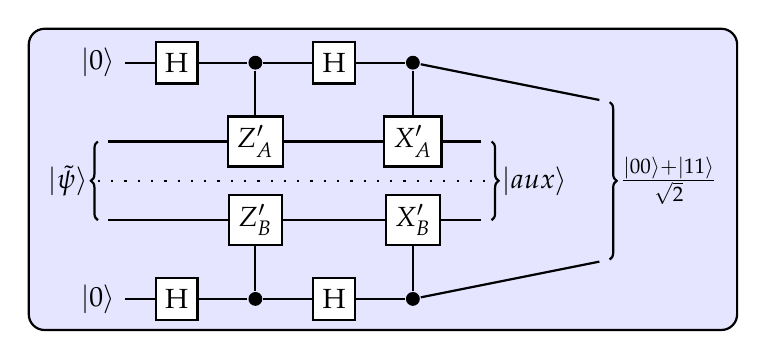
\begin{tikzpicture}[thick]
        %
        % `operator' will only be used by Hadamard (H) gates here.
        % `phase' is used for controlled phase gates (dots).
        % `surround' is used for the background box.
        \tikzstyle{operator} = [draw,fill=white,minimum size=1.5em] 
        \tikzstyle{phase} = [fill,shape=circle,minimum size=5pt,inner sep=0pt]
        \tikzstyle{surround} = [fill=blue!10,thick,draw=black,rounded corners=2mm]
        %
        % Bracket
        \draw[decorate,decoration={brace,mirror},thick] (0,-1) to
    	node[midway,left] (bracket1) {$\ket{\tpsi}$}
    	(0,-2);
        % Qubits
        \node at (0,0) (q1) {$\ket{0}$};
        \node at (0,-1) (q2) {};
        \node at (0,-2) (q3) {};
        \node at (0,-3) (q4) {$\ket{0}$};
        %
        % Column 1
        \node[operator] (op11) at (1,0) {H} edge [-] (q1);
        \node[operator] (op14) at (1,-3) {H} edge [-] (q4);
        %
        % Column 3
        \node[phase] (phase11) at (2,0) {} edge [-] (op11);
	\node[operator] (op22) at (2,-1) {$Z_A'$} edge [-] (q2);
	\node[operator] (op23) at (2, -2) {$Z_B'$} edge[-] (q3);
        \node[phase] (phase14) at (2,-3) {} edge [-] (op14);
        \draw[-] (phase11) -- (op22);
        \draw[-] (phase14) -- (op23);
        %
        % Column 4
        \node[operator] (op31) at (3,0) {H} edge [-] (phase11);
        \node[operator] (op34) at (3,-3) {H} edge [-] (phase14);
        %
        % Column 5
        \node[phase] (phase21) at (4,0) {} edge [-] (op31);
	\node[operator] (op42) at (4,-1) {$X_A'$} edge [-] (op22);
	\node[operator] (op43) at (4, -2) {$X_B'$} edge[-] (op23);
        \node[phase] (phase24) at (4,-3) {} edge [-] (op34);
        \draw[-] (phase21) -- (op42);
        \draw[-] (phase24) -- (op43);
        %
        % Column 6
        \node (end2) at (5,-1) {} edge [-] (op42);
        \node (end3) at (5,-2) {} edge [-] (op43);
        %
        % Bracket
        \draw[decorate,decoration={brace},thick] (5,-1) to
    	node[midway,right] (bracket) {$\ket{aux}$}
    	(5,-2);
        %
        % Column 7
        \node (end1) at (6.5,-0.5) {} edge [-] (phase21);
        \node (end4) at (6.5,-2.5) {} edge [-] (phase24);
        % Dashed line
        \draw[loosely dotted] (0,-1.5) -- (5,-1.5);
        % Bracket
        \draw[decorate,decoration={brace},thick,] (6.5,-0.5) to
    	node[midway,right] (bracket2) {$\frac{\ket{00}+\ket{11}}{\sqrt{2}}$}
    	(6.5,-2.5);
        %
        % Background Box
        \begin{pgfonlayer}{background} 
        \node[surround] (background) [fit = (q1) (op14) (bracket1)(bracket2)] {};
        \end{pgfonlayer}
        %
        \end{tikzpicture}
	\caption{The isometries $\Phi_A$ and $\Phi_B$.}
\end{figure}
To bound $e_{xy} := \norm{ (\Phi_A\x\Phi_B) (\tA_x \x \tB_y) \ket{\tpsi} - \ket{junk} \x (A_x\x B_y) \ket{\EPR{2}}}$,
there are some intermediate steps. Since the derivations are the same as in Ref.~\cite{bamps2015}, 
we only record the key relations here.
\begin{align*}
	&\norm{(Z_B' - Z_B) \ket{\tpsi}} \leq \frac{\sqrt{s}}{c} \sqrt{\epsilon},\\
	&\norm{(Z_B' - Z_A') \ket{\tpsi}} \leq 2 \frac{\sqrt{s}}{c}\sqrt{\epsilon}, \\
	&\norm{(X_B' - X_B) \ket{\tpsi}} \leq \frac{c+1}{s^{3/2}} \sqrt{\epsilon} := \delta_1 \sqrt{\epsilon},\\
	&\norm{(X_B'Z_B'+ Z_B'X_B')\ket{\tpsi}} \leq [\frac{2\sqrt{s}}{c} + \frac{2}{\sqrt{s}} + 2\delta_1 + 
	(\sqrt{2}+\frac{1}{c})(2\frac{\sqrt{s}}{c}+\frac{1+c+s}{c\sqrt{s}})]\sqrt{\epsilon}
	:= \delta_2 \sqrt{\epsilon}.
\end{align*}
Then we can calculate that 
\begin{align*}
	&e_{00} = e_{10} = 2\delta_2 \sqrt{\epsilon}\\
	&e_{20} = 2(\frac{1+c+s}{c\sqrt{s}} + \delta_2) \sqrt{\epsilon}\\
	&e_{01} = e_{02} = e_{11} = e_{12} = [\sqrt{s}+s(2\frac{1+c+s}{c\sqrt{s}} + \delta_1) + 2\delta_2]\sqrt{\epsilon}\\
	&e_{21} = e_{22} = [2\frac{1+c+s}{c\sqrt{s}} + \sqrt{s}+s(2\frac{1+c+s}{c\sqrt{s}} + \delta_1) + 2\delta_2]\sqrt{\epsilon},
\end{align*}
so an upper bound of the error is that
\begin{align}
	\forall x,y \in \{0,1,2\}, e_{xy} \in O((\frac{1}{c^2s^{1/2}} + \frac{1}{s^{3/2}})\sqrt{\epsilon}).
\end{align}
\end{proof}


\end{document}
